% !TEX program = xelatex
\documentclass[type=doctor]{fduthesis}
\fdusetup{
  style = {
    footnote-style = xits,
    bib-backend = bibtex,
    bib-resource = {reference.bib},
  },
}



\usepackage{enumerate}

% 自定义引用样式，支持可选参数
\NewDocumentCommand{\mycite}{o m}{%
  \IfNoValueTF{#1}
    {\scalebox{1.2}[1.2]{\raisebox{-0.70ex}{\cite{#2}}}}
    { \scalebox{0.9}[0.9]{\raisebox{0.10ex}{\textnormal{[#1, {\scalebox{1.3}[1.3]{\raisebox{-0.80ex}{\citealp{#2}}}}]}}}}}


\usepackage{xcolor}
\usepackage{hyperref}
\hypersetup{
    colorlinks=true, % 启用彩色链接
    linkcolor=black,  % 普通内部链接的颜色
    citecolor=black,  % 引用链接的颜色
    filecolor=black,  % 打开本地文件的链接颜色
    urlcolor=black    % 链接到URL的颜色
}

% 确保在导言区后期再重新设置一次
\AtEndPreamble{%
    \hypersetup{
        colorlinks=true,     % 启用彩色链接
        linkcolor=black,     % 普通内部链接的颜色
        citecolor=blue,     % 引用链接的颜色
        filecolor=green,     % 本地文件的链接颜色
        urlcolor=red,      % URL 链接的颜色
    }
}




\usepackage{amsmath}
\DeclareMathOperator{\codim}{codim}
\DeclareMathOperator{\dimension}{dim}
\DeclareMathOperator{\di}{div}
\DeclareMathOperator{\rank}{rank}
\DeclareMathOperator{\ricci}{Ricci}
\DeclareMathOperator{\dist}{dist}
\DeclareMathOperator{\hess}{Hess}
\DeclareMathOperator{\supp}{supp}
\DeclareMathOperator{\aut}{Aut}
\DeclareMathOperator{\id}{Id}

\DeclareMathOperator{\im}{Im}

\def\zz{{\mathbb Z}}
\def\rr{{\mathbb R}}
\def\cc{{\mathbb C}}
\def\qq{{\mathbb Q}}
\def\nn{{\mathbb N}}
\def\ss{{\mathbb S}}
\def\hh{{\mathbb H}}
\def\oo{{\infty}}
\def\db{{\bar{\partial}}}

\newcommand{\la}{\langle}
\newcommand{\ra}{\rangle}

\newcommand{\dif}{\mathop{}\!\mathrm{d}} % unicode-math 
\usepackage{wrapfig}




\begin{document}

\title{多复变}
\author{授课老师:陈伯勇}
\date{2021年 秋}
\maketitle



% 前置部分包含目录、中英文摘要以及符号表等
% \frontmatter

% 目录
\tableofcontents

\newpage
\section*{导引}
\begin{enumerate}
  \item 研究对象: 全纯函数, 全纯映射的分析与几何
  \item 源头: 椭圆函数的研究(Riemann, Weierstrass, Poincar\'e)
  \item 奠基人: Weierstrass, Poincar\'e 
  \item 本质现象: \begin{enumerate}
    \item Hartogs延拓现象
    \item Poincar\'e 定理
    \item Fatou-Bieberbach: $ \cc^2 \xrightarrow{F \text{双全纯}} F(\cc^2) \subset \cc^2 $, $ \cc^2 \setminus F(\cc^2) $有内点.
  \end{enumerate}
  \item 拟凸性(Levi), 多次调和函数(Oka, Lelong)
  \item Levi问题: $ \text{全纯域} \iff \text{拟凸性}$. $ \Rightarrow $ 平凡, Oka解决反向问题. (\textit{春宵十话})
  \item 代数拓扑的引入(层 + 上同调), Cartan-Serre
  \item PDE ($ \db $-方程的$L^2$-估计)
  \item 非线性方法的引入(复Mong\'e-Amper\'e算子)
  \item Bergman核. Bergman度量, Kobayashi度量.
\end{enumerate}
References:
\begin{enumerate}[1)]
  \item H\"ormander
  \item Krants SCV
  \item 涂振汉
  \item 张锦豪
\end{enumerate}

\begin{remark}
  本文根据课堂笔记整理而成; 
   另外, 关于本文的彩色文字:
    \begin{itemize}
     \item \textcolor{red}{红色}和\textcolor{blue}{蓝色}为老师的注释,
     \item \textcolor{purple}{紫色}为整理者的注解.
  \end{itemize}
\end{remark}



%%% 符号表
\begin{notation}[ll]
  $\Re$                  & 实部        \\
  $\Im$        & 虚部        \\
  $\Delta $            & $\cc$ 上的开单位圆盘  \\
  $P(c,r)=\prod_{j} \Delta(c_j,r_j)$      & $\cc^n$ 中的多圆柱(或多圆盘, 定义1.3)  \\
  $B(c,r)$        & $\cc^n$ 中的超球 (定义1.2)    \\
  $B^n$        & $\cc^n$ 中的单位超球    \\
\end{notation}






% 主体部分是论文的核心
\mainmatter



\chapter{全纯函数}
\section{定义, 基本性质}

\subsection{复欧式空间}


\begin{definition}[复欧式空间]
  $\rr^{2n}$-$2n$维实欧式空间, $x=(x_1,\dots,x_{2n})$. 令$z_\nu=x_\nu +i x_{n+\nu },~ 1\leq \nu \leq n.$   令$z=(z_1,...,z_n).$ 称$(\rr^{2n},z) $为复欧式空间, 记为$\cc^n$.
\end{definition}
\begin{enumerate}
  \item $z,w \in \cc^n, \alpha ,\beta \in \cc, \alpha z +\beta w =(\alpha z_1 +\beta w_1,\dots, \alpha z_n +\beta w_n)$.
  \item 复内积:$\la z, w\ra=\sum_{\nu =1}^{n}z_\nu \bar w_\nu  $, $|z|=\sqrt{\la z, z\ra }$
  \item $\Re (z_\nu \cdot \bar{w}_\nu )= x_\nu u_\nu +x_{n+\nu }u_{n+\nu }$, $\Rightarrow  $ $\Re (\la z, w\ra ) $即为实内积.
\end{enumerate}

\begin{definition}[超球]
  $B(c,r):=\{z\in \cc^n| |z-c|<r\}$.
\end{definition}
\begin{definition}[多圆柱]
  $P(c,r):=\{z \in \cc^n| |z_\nu -c_\nu| <r, 1 \leq \nu \leq n \}=\prod_{\nu =1}^{n} \Delta (c_\nu ,r)$. 其中, $\Delta $为圆盘.
\end{definition}
\begin{remark}
  \textcolor{purple}{有时也可取 $r=(r_1,\dots,r_n)$.} 
\end{remark}

$\rr^{2n} \to \cc^n ,~
x \mapsto (z,\bar{z}) $ 为一一对应, 故所有的函数$f(x)$可以写成$f(z,\bar{z}) $的形式, 简单起见, 记为$f(z)$.
\begin{definition}
  设$f \in C^1$, 定义
  \begin{align*}
    \frac{\partial f}{\partial z_\nu }:=\frac{1}{2}(\frac{\partial f}{\partial x_\nu }  +\frac{1}{i}\frac{\partial f}{\partial x_{n+\nu }} ) \\
    \frac{\partial f}{\partial \bar z_\nu }:=\frac{1}{2}(\frac{\partial f}{\partial x_\nu }  -\frac{1}{i}\frac{\partial f}{\partial x_{n+\nu }} )  \\
  \end{align*} 
\end{definition}
复合函数求导: $F=(f_1,\dots,f_m)$,
\begin{align*}
  \frac{\partial g \circ F}{\partial z_\nu }=\sum_{j =1}^{n}\frac{\partial g}{\partial w_j} \frac{\partial f^j}{\partial z_\nu } +\frac{\partial g}{\partial \bar w_j} \frac{\partial \bar f^j}{\partial z_\nu }  \\
  \frac{\partial g \circ F}{\partial \bar z_\nu }=\sum_{j =1}^{n}\frac{\partial g}{\partial w_j} \frac{\partial f^j}{\partial \bar z_\nu } +\frac{\partial g}{\partial \bar w_j} \frac{\partial \bar f^j}{\partial \bar z_\nu } \\
\end{align*} 
设$f=u+iv$, 则
\begin{align*}
  df=& du+idv\\
  =& \sum_{\nu =1}^{2n} \frac{\partial u}{\partial x_\nu }dx_\nu +i \sum_{\nu =1}^{2n}\frac{\partial v}{\partial x_{\nu }}dx_\nu   \\
  =& \cdots\\
  =& \sum_{\nu =1}^{n} \frac{\partial f}{\partial z_\nu }dz_\nu + \sum_{\nu =1}^{n}\frac{\partial f}{\partial \bar z_{\nu }}d\bar z_\nu \\
  := &\underbrace{\partial f}_{(1,0)}  + \underbrace{\bar \partial f}_{(0,1)}.
\end{align*} 
\begin{align*}
  d^2f=& d(\sum_{\nu }\frac{\partial f}{\partial x_\nu } dx_\nu )\\
  =& \sum_{\nu ,\mu } \frac{\partial^2 f }{\partial x_\nu  \partial x_\mu } dx_\mu \wedge dx_\nu \\
  =& \sum_{\mu <\nu } +\sum_{\mu >\nu }\\
  =&0.
\end{align*} 
\begin{equation*}
  \begin{aligned}
    0=d^2=&(\partial+\bar{\partial})^2\\
    =& \underbrace{\partial^2}_{(2,0)} +\underbrace{\partial \bar \partial}_{(1,1)}+ \underbrace{\bar \partial \partial}_{(1,1)} +\underbrace{\bar{\partial}^2}_{(0,2)}
  \end{aligned} 
\end{equation*}
$\Rightarrow \partial^2=\bar{\partial}^2=0,\partial \bar \partial+\bar \partial \partial=0.$ 

\subsection{全纯函数}
\begin{definition}
  设$U \subset \cc^n $为开集, 若
  \begin{enumerate}[1)]
    \item $f \in C(U)$;
    \item $f$关于每个分量$z_1,\dots,z_n $分别全纯,
  \end{enumerate}
  那么称$f$为$U$上的全纯函数, 记为$f \in \mathcal{O}(U)$. (\textcolor{blue}{$\leftarrow$为了纪念Oka}).
\end{definition}
\begin{remark}
    \begin{align*}
      f \in \mathcal{O}(U) &\iff  \frac{\partial f}{\partial \bar z_\nu } =0, \quad \forall \nu =1,\dots,n\\
      &\iff  \bar{\partial}f=0\\
      & \qquad \quad \updownarrow \\
      & \text{Cauchy-Riemann 方程}
    \end{align*} 
\end{remark}
\subsubsection{h原理, 整体性; 幂级数:局部性}
\begin{example}
  \begin{equation*}
    \left\{ 
    \begin{aligned}
      \Delta u=0\\
     \Delta v=0 \\
    \end{aligned} \quad, 
    \right.
    \text{but} \quad \Delta (uv)\neq 0.
  \end{equation*}
\end{example}
\begin{property}
    \begin{enumerate}
      \item $f,g \in \mathcal{O}(U) \Rightarrow f \pm g \in \mathcal{O}(U), fg \in \mathcal{O}(U)$;
      \item 全纯函数的复合也是全纯的.
    \end{enumerate}
\end{property}
\begin{example}
  $p(z):=\sum_{|\alpha |\leq m}^{}c_\alpha z^\alpha=\sum_{|\alpha |\leq m}^{}c_{\alpha_1 \dots \alpha _n} z_1^{\alpha_1 } \dots z_n^{\alpha _n} \in \mathcal{O}(\cc^n)$.

  $e^{p(z)},~\sin (p(z)) \in \mathcal{O}(\cc^n)$.
\end{example}

\begin{theorem}[Osgood]
    $f \in L^{\infty }_{loc}(U)$且$\bar{\partial }f=0 $ $\Rightarrow f \in \mathcal{O}(U). $ 
\end{theorem}
\begin{proof}
  只要证$f\in C(U)$.
  设$P(w,r) \subset \subset U$, $|f|\leq M$于$P(w,r)$.
  \begin{align*}
    f(z)-f(w)=& f(z_1,...,z_n)-f(w_1, z_2,...,z_n)\\
    &+ f(w_1,z_2,...,z_n)-f(w_1,w_2,z_3,...,z_n)\\
    & \cdots \\
    &+f(w_1,...,w_{n-1},z_n)-f(w_1,...,w_n).
  \end{align*} 
  由Schwarz引理,
  \begin{align*}
    |f(w_1,...,w_\nu ,z_{\nu +1},...,z_n)- f(w_1,...,w_{\nu+1} ,z_{\nu +2},...,z_n)| \leq \frac{2M}{r}|z_{\nu +1}-w_{\nu +1}|.
  \end{align*} 

  \fbox{\textbf{Schwarz引理}: $f \in \mathcal{O}(\Delta ),|f|\leq 1,f(0)=0 \Rightarrow |f(z)|\leq |z|.$}

作共形映射$h:\Delta \to \Delta (w_{\nu +1},r), \zeta \mapsto w_{\nu +1}+r \zeta .$
作
$$F(\zeta ):=\frac{1}{2M}[f(w_1,...,w_\nu ,h(\zeta ), z_{\nu +2},...,z_n)-f(w_1,...,w_\nu ,h(0 ), z_{\nu +2},...,z_n)],$$
$\Rightarrow $ $|F(\zeta )|\leq 1,F(0)=0. $ 取$\zeta =\frac{1}{r}(z_{\nu +1}-w_{\nu +1})$.
\end{proof}

\begin{theorem}[Hartogs (\textcolor{blue}{$\leftarrow$被纳粹逼自杀})]
   若$f$关于各个分量分别全纯, 则$f\in \mathcal{O}(U)$. 
\end{theorem}

\begin{example}
  $f(x_1,x_2)= \begin{cases}
    \frac{x_1x_2}{x_1^2+x_2^2} &\text{} (x_1,x_2) \neq 0\\
    0 &\text{} (x_1,x_2) = 0\\
  \end{cases} $ 
  关于各个分量解析, 但是$f \notin C(\rr^2)$.
\end{example}

\begin{theorem}[最大模定理]
    $\Omega \in \cc^n$区域, $f \not \equiv const$. 
    $\Rightarrow $ $f$不能在$\Omega $内部取到最大模.    
\end{theorem}
\begin{proof}
  $E:=\{x \in | |f(x)|=\max_{\Omega } |f|\}$,  利用连通性 $\Rightarrow $ $E=\emptyset ~ \text{or} ~ \Omega $. 
\end{proof}

\subsection{Cauychy积分公式}
\noindent $P(c,r)=\prod_{j} \Delta(c_j,r_j)$\\ 
$T:=\prod_{j} \partial \Delta(c_j,r_j)$ 为$P$的特征边界.\\
设$f \in \mathcal{O}(P(c,r)) \cap C(\overline{P(c,r)})$, 则
$$  f(z)=\frac{1}{(2 \pi i)^n} \int_{T} \frac{f(\xi )}{\xi -z} d \xi  $$   
$$  f^{\alpha }(z)=\frac{\alpha !}{(2 \pi i)^n} \int_{T} \frac{f(\xi )}{(\xi -z)^{\alpha +1}} d \xi  $$  
\begin{proof}
  \dots
\end{proof}

\begin{property}
  设 $f \in \mathcal{O}(P(c,r))$.
  \begin{enumerate}
    \item $f^\alpha  \in \mathcal{O}(P(c,r))$.
    \item Cauchy不等式: $f^\alpha (c) \leq \frac{\alpha !}{r^\alpha } \max |f|$.
    \item If $f \in C(\overline{P(c,r)})$, $\max_{P(c,r)}|f|=\max_{T}|f|$.  
  \end{enumerate}
\end{property}

\begin{definition}
  设$\Omega \subset \cc^n$为一个有界区域, 称满足
  $$ \max_{E}|f|=\max_{\bar \Omega }|f| $$
  的最小闭子集$E \subset \partial \Omega $为$\Omega $的Shilov边界. (\textcolor{blue}{$\leftarrow$ Banach代数中的重要概念.})
\end{definition}

\begin{example}
  球的Shilov边界为球面.
  \begin{proof}
    考虑单位球$B^n$, 设$\zeta \in \partial B^n, z \in B^n$.\\
    令$f(z)=e^{\la z,\zeta  \ra } \in \mathcal{O}(\cc^n)$.
  \end{proof}
\end{example}
\begin{example}
  $P(c,r)$的Shilov边界为$T$.
  \begin{proof}
    取外接球.
  \end{proof}
\end{example}

\begin{theorem}[Weierstrass]
  $\{f_j\} \in \mathcal{O}(\Omega )$ 且 $f_j \xrightarrow{\text{内闭一致}}f$, \\
  $\Rightarrow $ $f \in \mathcal{O}(\Omega )$,   且 $f^\alpha_j  \xrightarrow{\text{内闭一致}}f^\alpha $.
\end{theorem}
\begin{proof}
  \dots
\end{proof}

\begin{theorem}[Montel]
  设$\mathcal{F} \in \mathcal{O}(\Omega )$ 内闭一致有界.\\
  $\Rightarrow $ $\forall \{f_j\} \subset \mathcal{F}$, $\exists$ 内闭匀敛的子列.   
\end{theorem}
\begin{proof}
  根据Arzela-Ascoli, 只需证 $\mathcal{F}$在 $\forall$ 紧子集上等度连续.\\
  紧集由有限个多圆柱覆盖.\\
利用Osgood定理.
\end{proof}

\begin{theorem}[Liouville]
    $f \in \mathcal{O}(\cc^n) \cap L^{\infty }(\cc^n)$.\\
    $\Rightarrow $ $f=const.$   
\end{theorem}
\begin{proof}
 方法一: 单复变Liouville定理;\\
  方法二: Cauychy积分公式.
\end{proof}

\noindent \textcolor{purple}{解析性(幂级数展开):}\\
$f \in \mathcal{O}(P(c,r))\cap C(\overline{P(c,r)})$,\\
$\Rightarrow $ $\forall z \in P(c,r)$:
\begin{equation*}
  \begin{aligned}
    f(z)=& \frac{1}{(2 \pi i)^n} \int_{T(c,r)} \frac{f(\xi )}{\xi -z} d \xi \\
    =& \frac{1}{(2 \pi i)^n} \int_{T} \frac{f(\xi )}{(\xi_1 -z_1) \cdots (\xi_n -z_n)} d \xi_1 \dots d\xi_n\\
    =& \frac{1}{(2 \pi i)^n} \int_{T} \frac{f(\xi )}{(\xi -c)\left(1-\frac{z-c}{\xi -c}\right)} d \xi\\
    =& \sum_{\alpha } \frac{f^\alpha (c)}{\alpha !}(z-c)^\alpha 
  \end{aligned} 
\end{equation*}   
由Cauchy不等式 $\Rightarrow $ 级数内闭匀敛. (\textcolor{purple}{注:} $\frac{1}{1-x}=1+x+x^2+\dots, \forall |x| <1 .$)

\begin{theorem}[唯一性]
    $\Omega \in \cc^n$区域, $f \in \mathcal{O}(\Omega )$.\\
    若存在非空开集$U \in \Omega $ s.t. $f|_U=0$ $\Rightarrow $ $f \equiv 0 \quad \Omega .$  
\end{theorem}
\begin{proof}
  $E:=\{z \in \Omega | f^{\alpha }(z)=0, \forall \alpha \}$ 为闭集. 只要证$E$为开集.(幂级数展开.) 
\end{proof}

\begin{remark}
   许多椭圆方程的解也满足唯一性. 
\end{remark}

\begin{example}
  $P(0,1)$: 单位多圆柱.
  $E:=\{z\in P(0,1)|\im (z_j)=0, \forall j\}$.\\
   设$f \in \mathcal{O}(P(0,1))$, 则
   $$ f(z)=\sum_{\alpha }c_\alpha z^\alpha  .$$ 
   令$x=\Re (z)$ $\Rightarrow $ $f(x)=\sum_\alpha c_\alpha x^\alpha .$  若$f|_E=0$, $\Rightarrow $ $f \equiv 0$ 于 $P(0,1)$. 此时$\dim_{\rr} E=n$.  
\end{example}

\begin{definition}
  称$A\in \Omega $为一个唯一性集, 若$f|_A=0 ~ \Rightarrow f \equiv 0 \quad \forall f \in \mathcal{O}(\Omega ).$
\end{definition}

\begin{theorem}[Vitali]
    $A\in \Omega $唯一性集, $\{f_\nu \} \subset \mathcal{O}(\Omega )$ 内闭一致有界, 且 $f_\nu $在$A$上点态收敛.\\
    $\Rightarrow $ $f_\nu $内闭匀敛.   
\end{theorem}
\begin{proof}
  假设存在紧集$K \subset \Omega $, 子列 $\{\nu _k\}, \{\mu _k\}, \{z_k\} \subset K$ and $\delta >0$ , s.t.
  $$ |f_{\nu _k}(z_k) -f_{\mu _k}(z_k) | \geq \delta \quad \forall k .$$ 
  由Montel定理, 存在$\{\nu _k\}, \{\mu _k\}$ 子列, (仍记为$\{\nu _k\}, \{\mu _k\} $), s.t. 
  $$ f_{\nu _k} \to f, f_{\mu _k} \to g \in \mathcal{O}(\Omega ).$$
  另外, 由Bolzano-Weierstrass定理, 存在$\{z_k\}$子列(仍记为$\{z_k\}$), s.t. 
  $$ z_k \to z_0. $$
  因为
  \begin{align*}
    |f_{\mu _k}(z_k) -f_{\mu _k}(z_0) | \leq M|z_k-z_0| \\
    |f_{\nu _k}(z_k) -f_{\nu _k}(z_0) | \leq M|z_k-z_0|
  \end{align*} 
  \textcolor{blue}{(由Osgood证明)}.
\end{proof}

\begin{definition}
  $\Omega \subset \cc^n$区域.  若$\forall z \in \Omega $, $\forall \xi \in \partial \Delta $, 有$\xi \cdot z \in \Omega $, 则称$\Omega $为一个圆形域.\\
  若进一步, $\forall z \in \Omega $, $\forall \xi \in \bar \Delta $, 有$\xi \cdot z \in \Omega $, 则称$\Omega $为一个完备圆形域.\\
  若$\forall z \in \Omega $, $\forall \xi_1,\dots,\xi _n \in \partial \Delta $, 有$(\xi_1 \cdot z_1,\dots,\xi_n \cdot z_n) \in \Omega $, 则称$\Omega $为一个Reinhardt域.\\
  若$\forall z \in \Omega $, $\forall \xi_1,\dots,\xi _n \in \bar \Delta $, 有$(\xi_1 \cdot z_1,\dots,\xi_n \cdot z_n) \in \Omega $, 则称$\Omega $为一个完备Reinhardt域.
\end{definition}
\begin{remark}
  Reinhardt域 $\Rightarrow $  圆形域.
\end{remark}

\begin{example}
  \begin{enumerate}[1).]
    \item $\{z : |z|<r\}$, $\{z: z_j <|r_j|,1 \leq j \leq n\}$  $\Rightarrow $ Reinhardt域.
    \item  $\{(z_1,z_2):|z_1|^2+\frac{1}{|z_2|^2}<1\}$ $\Rightarrow $ Reinhardt域, 非完备.
    \item $\{(z_1,z_2):|z_1^2+z_2z_1+z_2^2|< 1\}$   $\Rightarrow $ 完备圆形, 非Reinhardt. 
  \end{enumerate}
\end{example}

\begin{theorem}[H.Cartan]
  完备圆形域上的全纯函数可以展开为内闭匀敛的幂级数. 
\end{theorem}
\begin{proof}
  $\exists P(0,r) \subset \subset \Omega $, s.t. 
  $$ \begin{aligned}
    f(z)=& \sum_{j=0}^{ \infty }\sum_{|\alpha |=j}^{} c_\alpha z^\alpha \\
    := & \sum_{j=0}^{\infty } P_j(z)
  \end{aligned}  $$ 
  $w \in \Omega $, $f(\xi \cdot w)$为$\xi \in \bar \Delta $  上的全纯函数,
  $$ \Rightarrow \quad f(\xi w)=\sum_{j=0}^{ \infty }c_j(w)\xi ^j. $$
  当$|\xi| <<1 $时, $\xi w \in P(0,r)$,
  $$ \begin{aligned}
    &\Rightarrow  \quad P_j(w)=c_j(w)\\
    &\Rightarrow  \quad f(w)=\sum_{j=0}^{\infty }P_j(w) \\
    & \Rightarrow \quad f  \text{点态收敛于 } \Omega .
  \end{aligned}  $$ 
  设$K \subset \Omega $紧集,
  $$ K':= \bar{\Delta } \cdot K=\{\xi z: \xi \in \bar{\Delta }, z\in K\}. $$
  则$K'$为紧集, 且$K \subset K'$. 取$\delta <1$及紧集$K' \subset K'_{\delta } \subset \Omega $, s.t. $\frac{\eta }{\delta } \cdot w \in K'_{\delta }$, $\forall \eta \in \bar{\Delta },w \in K$.
  $$ f(\frac{\eta }{\delta } \cdot w) =\sum \frac{P_j(w)}{\delta ^j}\eta ^j, \quad \eta \in \bar{\Delta }$$  
  $$ \overset{\text{Cauchy不等式}}{\Rightarrow} \quad \left| \frac{P_j(w)}{\delta ^j} \right| \leq \max_{K'_{\delta }}|f|=C_\delta .$$
  \textcolor{purple}{Using $\left| \sum_{j=0}^{\nu }P_j(w) \right| \leq C_\delta \frac{1}{1-\delta } $. (?) }
\end{proof}

\begin{theorem}
   Reinhardt域上的全纯函数可以展开为内闭匀敛的Laurent级数. 
\end{theorem}
\begin{proof}
  固定$w\in \Omega \setminus \{z_1 \cdots z_n=0\}$. 则存在$\delta >0$, s.t.
  $$ A(w,\delta ):=\prod_{j=1}^{n}\{z_j: 0<|w_j|-\delta <|z_j|<|w_j|+\delta  \} \subset \subset \Omega .\quad (\textcolor{blue}{\text{Reinhardt 性质}}) $$
  依次利用单变量Laurent级数展开
  $$ f(z)=\sum_{\alpha \in \zz^n}^{}c_\alpha(w) z^\alpha  ,$$
  其中, $c_\alpha = \frac{1}{(2 \pi i)^n} \int_{\prod_{j=1}^{n} \partial \Delta (0,|w_j|)} \frac{f(\xi )}{\xi^{\alpha +1}} d \xi $.
  
  设$w'\in \Omega \setminus \{z_1 \cdots z_n=0\}$另一点.\\
  $\Rightarrow $ $c_\alpha (w)=c_\alpha (w')$ 与 $A(w,\delta ) \cap A(w',\delta ') $   \\
  $\Rightarrow $ $c_\alpha $局部为常数.\\
  $\because $  $c_\alpha (w)$连续且$\Omega \setminus \{  z_1 \cdots z_n=0\}$ 连通, (\textcolor{blue}{练习})\\
  $ \therefore$ $c_\alpha (w) \equiv c_\alpha $.  
\end{proof}

\subsection{Hartogs延拓现象}
\noindent $\Omega $区域, $a \in \partial \Omega $.\\
$f(z)=\frac{1}{z-a} \in \mathcal{O}(\Omega )$, 但$f$ 不能延拓过$a$.  
\begin{example}[Hartogs]
  设$0<r_1,r_2<1$, $\Omega :=(\Delta _{r_1} \times \Delta )\cup (\Delta \times  \Delta \setminus \bar{\Delta }_{r_2}) \subset \cc^2$. \\
  $\Rightarrow $ $\forall f \in \mathcal{O}(\Omega )$可全纯延拓到$ \Delta ^2$.   
  \begin{figure}[h!]
    \centering
    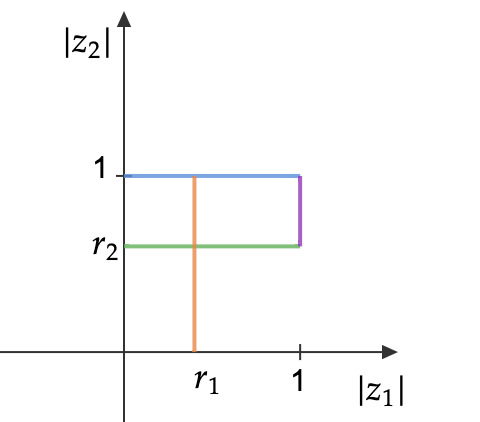
\includegraphics[width=0.4\textwidth]{Hartogs.jpg}
    \caption{Hartogs图}
    \end{figure}
  
  \begin{proof}
    令$r_2<r_3<1$, 对于$(z_1,z_2) \in \Delta \times \Delta _{r_3}$, 令
    $$ F(z_1,z_2)= \frac{1}{2\pi i} \int_{|\xi |=r_3}^{} \frac{f(z_1,\xi )}{\xi -z_2} d\xi,$$
    $\Rightarrow $ $F \in \mathcal{O}(\Delta \times \Delta _{r_3})$, 且 $F=f$ 于 $ \Delta_{r_1} \times \Delta _{r_3}$. 由唯一性定理 $\Rightarrow $ $F$ 为 $f$ 在 $ \Delta \times \Delta _{r_3}$上的全纯延拓.   
  \end{proof}
\end{example}

\begin{theorem}[Hartogs延拓定理]
    $\Omega $区域, $n \geq 2$. $K \subset \Omega $紧集且$\Omega \setminus K $连通.\\
    $\Rightarrow $ $\forall f \in \mathcal{O}(\Omega \setminus K)$可全纯延拓到$\Omega $.    
\end{theorem}
\begin{figure}[h!]
  \centering
  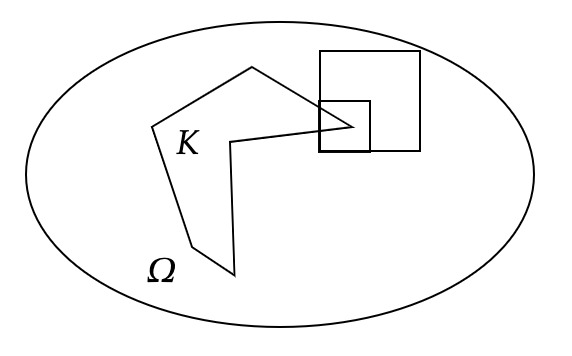
\includegraphics[width=0.4\textwidth]{Hartogs2.jpg}
  \caption{Hartogs的初等证明(Bochner给出完整的证明)}
  \end{figure}

\noindent\textbf{预备知识}:

\noindent 设$\Omega \subset \cc^n$为一区域, $v_1,...,v_n$为$\Omega $上$n$个函数. 称
$$ \frac{\partial u}{\partial \bar{z}_j}=v_j,\quad \forall  j=1,\dots,n  $$  
为非齐次Cauchy-Riemann方程.

令$v:=\sum_{j}^{}v_j d \bar{z}_j$ 为一 $(0,1)$-形式. 则 
$$ \bar{\partial}u=v, $$ 
$\because \quad \bar{\partial}^2u=0$, $\Rightarrow $  方程有解的必要条件为$ \bar{\partial}v=0. $

\begin{exercise}
$\bar{\partial}v=0 \iff \frac{\partial v_j}{\partial \bar{z}_k}=\frac{\partial v_k}{\partial \bar{z}_j}  $. 
\end{exercise}

\begin{lemma}[$\bar{\partial}$-Poincare引理 ]
  $n \geq 2 $, $v$: $\cc^n$中$C^{\infty }$-$(0,1)$形式且具有紧支集, $\bar{\partial}v=0$.\\
  $\Rightarrow $ $ \exists u \in C_{0}^{\infty }(\cc^n)$, s.t. $\bar{\partial}u=v$, 且 $u $ 在$\cc^n \setminus \supp(v)$   的无界连通分支上$\equiv 0 $.   
\end{lemma}

\begin{proof}[Hartogs延拓定理]
  取区域$\Omega ' \subset \subset \Omega , K \subset \Omega '.$ 取$\chi = C_0 ^{\infty }(\Omega ')$, $\chi \equiv 1$于$K $的某个领域. \\
  设$f \in \mathcal{O}(\Omega \setminus K)$. 令
  $$ v=\begin{cases}
     \bar{\partial}((1-\chi )f) &\text{} \Omega \setminus K\\
    0 &\text{} K \cup (\cc^n \setminus \Omega) \\
  \end{cases}  $$
  则$v$为 $\cc^n$中$C^{\infty }$-$(0,1)$形式且具有紧支集.\\
  $\Rightarrow \bar{\partial}u=v.$\\
  令 $F:=(1-\chi )f-u ~ \in C^{\infty }(\Omega )$, $\bar{\partial}F=v-\bar{\partial}u=0 \quad \Omega $. \\
  $\Rightarrow $  $F \in \mathcal{O}(\Omega )$.\\
  在 $\Omega \setminus \Omega ' $上, $u=0,\chi =0.$ (\textcolor{purple}{$ \bar{\partial }f=0 \Rightarrow \supp(v) \subset \supp (\chi ) \subset \Omega '$}. )    \\
  $\Rightarrow $ $F=f$于$\Omega \setminus \Omega '$.\\
  由唯一性定理, $\Rightarrow $ $F=f$ 于 $\Omega \setminus  K$.       
\end{proof}

\begin{lemma}\label{le:12}
设 $v=g d \bar{z}, g \in C_0^{\infty }(\cc)$. 令 $u(z)=\frac{1}{2 \pi i} \int_{\cc}^{} \frac{g(\xi )}{\xi -z} d \xi \wedge d \bar{\xi }.$ \\
则 $u \in C^{\infty }( \cc)$且 $\bar{\partial }u=v.$     
\end{lemma}
\begin{proof}
  令 $\xi =z+r e^{i \theta }$. \\
  $\Rightarrow $ $d \xi \wedge  d \bar{\xi }=-2ir dr \wedge  d \theta  $ $\quad (d \xi = e^{i \theta } dr +r i e^{i \theta } d \theta , d \bar \xi = e^{-i \theta } dr -r i e^{-i \theta } d \theta)$  \\
  $\Rightarrow $ $ u(z)=- \frac{1}{\pi }\int_{0}^{+\infty } \int_{0}^{2 \pi } g(z+r e ^{i \theta }) e^{-i \theta } dr d \theta $\\
  $\Rightarrow $ $ u \in  C^{\infty }(\cc)$\\
  $$  
  \begin{aligned}
    \Rightarrow \quad \frac{\partial u}{\partial \bar{z}}=&- \frac{1}{\pi } \int_{0}^{+ \infty } \int_{0}^{2 \pi } \frac{\partial g}{\partial \bar{z}} (z+r e^{i \theta })dr  d \theta    \\
    \stackrel{\xi =re^{i \theta }}{= } &  \frac{1}{2 \pi  i} \int_{\cc}^{} \frac{\partial g(z+\xi )}{\partial \bar{z}} \frac{1}{\xi }  d \xi \wedge d \bar{\xi } \\
    =& \frac{1}{2 \pi  i} \int_{\cc}^{} \frac{\partial g(z+\xi )}{\partial \bar{\xi }} \frac{1}{\xi }  d \xi \wedge d \bar{\xi } \\
    =& \lim_{\epsilon  \to 0}  \frac{1}{2 \pi i} \int_{\cc \setminus \bar{\Delta }_{\epsilon }}^{} \frac{\partial g(z+\xi )}{\partial \bar{\xi }} \frac{d \xi \wedge d \bar{\xi }}{\xi }  \\
    =& -\lim_{\epsilon  \to 0}  \frac{1}{2 \pi i} \int_{\cc \setminus \bar{\Delta }_{\epsilon }} d_{\xi } \left( \frac{g(z+\xi )}{\xi }d \xi \right)   \\
    \stackrel{Stokes}{= } & -\lim_{\epsilon  \to 0}  \frac{1}{2 \pi i} \int_{\partial  \bar{\Delta }_{\epsilon }}   \frac{g(z+\xi )}{\xi }d \xi   \quad (\textcolor{purple}{\text{令} \xi =\epsilon e^{i \theta }})\\
    =& g(z).
  \end{aligned} 
  $$      ~
\end{proof}

\begin{proof}[$\bar{\partial }$-Poincar\'e引理 ]
  设 $v:=\sum v_j d \bar z_j$. 则令 $z'=(z_2,\dots, z_n)$,
  $$ u(z):= \frac{1}{2 \pi i} \int_{\cc}^{} \frac{v_1(\xi ,z')}{\xi -z_1} d \xi  \wedge  d \bar{\xi }.$$  
利用极坐标 $\Rightarrow $ $u \in  C^{\infty }(\cc^n)$.\\
$ \text{由引理}\ref{le:12} \Rightarrow   $  $\frac{\partial u}{\partial \bar{z}_1} =v_1$.  \\
对于 $j \geq 2$,
$$ \begin{aligned}
  \frac{\partial u}{\partial \bar{z}_j}=& \frac{\partial }{\partial \bar{z}_j}  \left(\frac{1}{2 \pi i} \int_{\cc}^{} \frac{v_1(z_1+\xi ,z')}{\xi } d \xi  \wedge  d \bar{\xi }\right)\\
  =& \frac{1}{2 \pi i} \int_{\cc} \frac{\partial v_1}{\partial \bar{z}_j}(z_1+\xi ,z') \frac{d \xi  \wedge  d \bar{\xi }}{\xi } \\
  \stackrel{\text{由相容性条件}}{=}& \frac{1}{2 \pi i} \int_{\cc} \frac{\partial v_j}{\partial \bar{z}_1}(z_1+\xi ,z') \frac{d \xi  \wedge  d \bar{\xi }}{\xi } \\
  =& \frac{\partial }{\partial \bar{z}_1} \left(\frac{1}{2 \pi  i} \int_{\cc} \frac{v_j(z_1+\xi ,z')}{\xi }  d \xi  \wedge  d \bar{\xi }\right) \\
  \stackrel{\text{由引理}\ref{le:12}}{=}& v_j(z), \qquad \Rightarrow \bar{\partial }u=v.
\end{aligned} 
 $$ 
 $\because ~ v=0$ 于 $\cc^n \setminus \supp v$, $\Rightarrow  u \in \mathcal{O}(\cc^n \setminus \supp v)$.\\

 \begin{figure}[htbp]
  \centering
  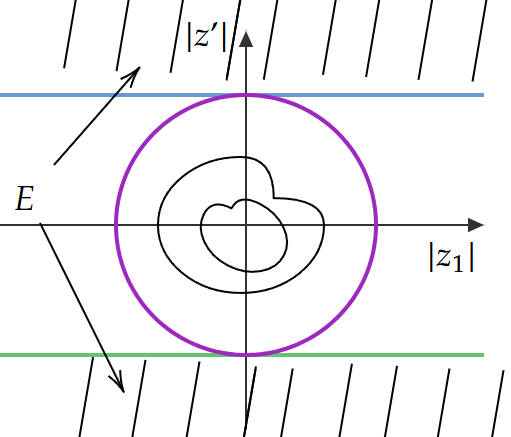
\includegraphics[width=0.4\textwidth]{DBarlem.jpg}
  \caption{$\db$-Poincare 引理证明}
\end{figure}
 取 $R>>1, \supp v \subset B(0,R)$, 则 $E=\{z \in \cc^n: |z'|>R \} \subset \cc^n \setminus B(0,R)$. 由 $u$的定义 $\Rightarrow $ $u|_E=0$ $ \overset{\text{唯一性}}{\Rightarrow}$ $u=0$ 于 $\cc^n \setminus \supp v $的无界连通分支.          
\end{proof}
 

\section{全纯映射}
$\Omega \subset \cc^n $ 区域, $F=(f_1,\dots,f_m)$为 $\Omega  \to \cc^n$的一个映射. 若 $\forall f_j \in \mathcal{O}(\Omega )$, 则$F$为一个全纯映射.
当$m=n$时, 则称
$$ J_{\cc}(F)=
\begin{vmatrix}
\frac{\partial f_1}{\partial z_1} & \cdots& \frac{\partial f_1}{\partial z_n}\\
\vdots & &  \vdots \\
\frac{\partial f_n}{\partial z_1} & \cdots& \frac{\partial f_n}{\partial z_n}\\
\end{vmatrix} $$
为$F$的复Jacobian. 

设 $ f_j=u_j+iu_{n+j}, j=1,\dots,n. \quad (z_j=x_j+ix_{n+j})$. 称 
$$ J_{\rr}(F)=
\begin{vmatrix}
\frac{\partial u_1}{\partial x_1} & \cdots& \frac{\partial u_1}{\partial x_{2n}}\\
\vdots & &  \vdots \\
\frac{\partial u_{2n}}{\partial x_1} & \cdots& \frac{\partial u_{2n}}{\partial x_{2n}}\\
\end{vmatrix} $$
为$F$的实Jacobian. 

\begin{proposition}\label{pro1}
$ J_{\rr} (F)=|J_{\cc}(F)|^2.$ 
\end{proposition}
\begin{corollary}
复流形可定向. 
\end{corollary}
\begin{proof}
  在 $ J_{\rr} $中第$n+r$行 $ \times i ~+$ 第$r$行, 利用 
  $$ \frac{\partial f_k}{\partial x_j} = \frac{\partial f_k}{\partial z_j} ,\quad \frac{\partial f_k}{\partial x_{n+j}}=i \frac{\partial f_k}{\partial z_j}   $$
  $$ \Rightarrow \quad  J_{\rr}=
  \left|
\begin{array}{c|c}
A & B \\
\hline
C & D
\end{array}
\right| $$
再将第$k$列 $ \times  -i$ $ + $ 第$n+k$列, 利用 
$$ \frac{\partial u_{n+j}}{\partial x_{n+k}} = \frac{\partial u_{j}}{\partial x_{k}}$$
$$ \Rightarrow \quad \left|
  \begin{array}{c|c}
  J_{\cc} & O \\
  \hline
  * & \bar{J}_{\cc}
  \end{array}
  \right| = \left| J_{\cc} \right|^2. $$ ~
\end{proof}

\begin{theorem}[隐函数定理]
 设 $ F(w,z)=(f_1(w,z),\dots,f_m(w,z)) $ 在 $ (0,0) $的某个领域内全纯, s.t. $ F(0,0)=0 $ 且 $ J_{\cc}(F)|_{(0,0)} \neq 0 $.\\
 $ \Rightarrow  $ $ \exists 0 \in \cc^n $ 的某领域上的全纯映射 $ w=w(z) $, s.t. $ w(0)=0 , F(w(z),z)=0$.
\end{theorem}
\begin{proof}
  令 $ w_k=u_k+iu_{n+k},z_k=x_k+i x_{n+k} $, 则 $ F(w,z)=0 $ 等价于下面 $ 2m $ 个实方程组
  $$\left\{  \begin{aligned}
    \Re F(u,x)=0 \\
   \Im F(u,x)=0 \\
  \end{aligned} \right. $$
  由命题 \ref{pro1} 及实隐函数定理 $ \Rightarrow  $ 
  $ \exists 0 \in \cc^n $的某个领域上的 $ C^{\infty } $ 映射 $ w $, s.t. 
  $$ w(0)=0, \quad F(w(z),z)=0. $$
  只需要证明 $ w $ 全纯:\\
  对方程 $ f_j(w(z),z)=0 $ 两边左边作用 $ \frac{\partial }{\partial \bar{z}_l}  $:
  $$ \sum_{k=1}^{m} \frac{\partial f_j}{\partial w_k} \frac{\partial w_k}{\partial \bar{z}_l} +\sum_{k=1}^{m} \frac{\partial f_j}{\partial \bar w_k} \frac{\partial \bar w_k}{\partial \bar{z}_l}=0$$
  $ \left(\left. \frac{\partial f_j}{\partial w_k}\right|_{(0,0)} \right)$为非异阵 $ \Rightarrow  $ $  \frac{\partial w_k}{\partial \bar{z}_l}=0 $于 $ 0 \in \cc^n $充分小的领域.
\end{proof}

\begin{corollary}[逆映射定理]
 $ U $ 为 $ w_0 \in \cc^n $ 的领域, $ G: U \to \cc^n $ 全纯. 且 $ z_0 =G(w_0), J_{\cc}(G)|_w \neq 0$. \\
 $ \Rightarrow  $ 在 $z_0 \in \cc^n$ 的某领域上$G^{-1}$ 存在且全纯.
\end{corollary}
\begin{proof}
  令 $ F(w,z)=G(w)-z $.
\end{proof}

\begin{corollary}
$ F:\Omega \subset \cc^n \to \cc^n  $全纯且 $ |J_{\cc}F|>0 $于 $ \Omega  $.\\
$ \Rightarrow  $ $ F $为一个开映射.
\end{corollary}
\begin{remark}
  \textcolor{blue}{单复变全纯 $ \Rightarrow  $ 开映射.}
\end{remark}

\begin{definition}
  $ F: \Omega  \subset \cc^n \to \Omega ' \subset \cc^n $ 为一个双射, 且$F^{-1} $ 全纯. 称 $F$ 为一个双全纯函数(Biholomorphic).

\noindent (\textcolor{blue}{由单复变启发, 对高维区域分类?})
\end{definition}
\begin{remark}
  $ \because F \circ F^{-1}=id $ $ \Rightarrow  $ $ J_{\cc} F \cdot J_{\cc}F^{-1}=1 $ $ \Rightarrow  $ $ |J_{\cc}F|>0 $. 反之, 若一个全纯映射$F $, s.t. $ |J_{\cc}F|>0 $, 则其局部为双全纯.
\end{remark}
\begin{example}[覆盖映射]
\begin{figure}[htbp]
  \centering
  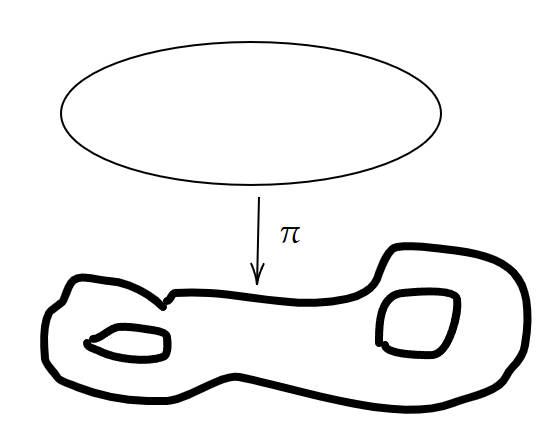
\includegraphics[width=0.4\textwidth]{Covering.jpg}
  \caption{覆盖映射}
\end{figure}  
\end{example}

\begin{theorem}[秩定理]
 $ \Omega \subset \cc^n $ 区域, $ 0 \in \Omega , F \in \mathcal{O}(\Omega ,\cc^m) $, s.t. $ F(0)=0 $
 且 $ F' $  的秩为常数 $ l. $
 则 $ \exists 0 \in \cc^n $ 以及 $ 0 \in \cc^m $ 领域上的双全纯映射 $ H,G $, s.t. $ G \circ F \circ H(w)=(w_1,\dots,w_l,0,\dots,0) $.
\end{theorem}
\begin{proof}
  设 $ F=(f_1,\dots,f_m) $
  不妨设 $ \det (\frac{\partial f_j}{\partial z_k} )_{1 \leq j,k \leq l}|_{0} \neq  0 $.
  定义全纯映射
  $$ A:\begin{cases}
   w_j=f_j(z)  &\text{} 1 \leq j \leq l\\
   w_j=z_j  &\text{} l+1 \leq j \leq n\\
  \end{cases}  $$
 $ \therefore $  $\exists 0 \in \cc^n $ 的某个领域上的 $ H=A^{-1} $.\\
$ \Rightarrow  $ $ A \circ H(w)=w $.\\
$ \Rightarrow  $ $ F \circ  H(w) = (w_1,\dots w_l, \tilde{f}_{l+1}(w),\dots, \tilde{f}_{m}(w))$ \\
 $ \because  $ $ F' $的秩为 $ l $, \\
 $ \Rightarrow  $ $ \frac{\partial \widetilde{f}_j}{\partial w_k} =0, \forall j,k >l $ 
 $$ \left|
  \begin{array}{c|c}
  J_{l \times  l} & O \\
  \hline
  * & \cdots 
  \end{array}
  \right|  $$
 $ \Rightarrow  $ $ \tilde{f}_j(w)= \tilde{f}_j(w_1,\dots, w_l) $.
 
 定义: $ G=(g_1,\dots,g_m) $
$$ \begin{cases}
  g_j(\xi )=\xi _j &\text{} j \leq l\\
  g_j(\xi )=\xi _j -\tilde{f}_j (\xi_1 ,\dots,\xi_l )&\text{} j>l\\
\end{cases}  $$
$ \Rightarrow  $ $ J_\cc(G)|_0 \neq 0 $ \\
$ \Rightarrow  $ $ G $ 在$0$ 的领域双全纯,
  且 $ G \circ F \circ H(w)=(w_1,\dots,w_l,0,\dots,0) $.
\end{proof}

\begin{lemma}[Schwarz引理]
 设 $ ||\cdot ||_1,||\cdot ||_2 $  为 $ \cc^n $ 中两个范数.
 $ B_1:=\{z \in \cc^n: ||z||_1 <1\} ,  B_2:=\{z \in \cc^n: ||z||_2 <1\}$
 若 $ F \in \mathcal{O}(B_1,B_2) $, s.t. $ F(0)=0 $.
 则 $ ||F(z)||_2 \leq ||z||_1 $.
\end{lemma}

\begin{example}
  $ ||z||_1 = \sqrt{|z_1|^2+\dots +|z_n|^2}$, 
  $ ||z||_2 =\max_{1 \leq j \leq n} |z_j| $.
\end{example}

\begin{theorem}[Poincare 定理]
 当 $ n \geq 2 $ 时, 单位球不双全纯同胚于单位多圆柱.
\end{theorem}
\begin{proof}
  $ F: \Delta^n \to  \mathbb{B}^n$. \\
  设 $ F(p)=0 $, 取 $ \phi _j \in \aut (\Delta ) $, s.t. $ \phi _j(p_j)=0 $. (\textcolor{blue}{单复变:$\aut (\Delta )=\{\text{莫比乌斯变换}\} $. $ \aut(\Omega )=\{f: \Omega \to \Omega \text{双全纯}\} $). }\\
  $ \Rightarrow  $ $ \phi := (\phi _1,\dots,\phi _n) \in \aut (\Delta ^n) $. \\
  令 $ G:=F \circ \phi ^{-1} $. 则 $ G $ 为双全纯且 $ G(0)=0 $. \\
  令 $ H=G^{-1} $, 对 $ G $ 以及$H$ 分别用 Schwarz引理 \\
  $ \Rightarrow  $ $ \sum |g_j(z)|^2=\max_{1\leq j \leq n}|z_j|^2  $.\\
  $ \because  $ 左边是 $ C^{\infty } $, 右边不是 $ C^{\infty } $. ($ \because  n \geq 2$.)
\end{proof}

\begin{lemma}[\textcolor{blue}{凸分析理论}]\label{le:14}
 设 $ ||\cdot|| $ 为 $ \cc^n $ 中的一个范数, $ z_0 \in \cc^n $.\\
 $ \Rightarrow  $ 存在一个复线性函数 $ l(z) $, s.t.
 $$ l(z_0)=||z_0||,\quad l(z) \leq ||z||, \forall  z. $$
\end{lemma}

\begin{proof}[Schwarz引理]
  $ \forall  z_0 \in B_1 \setminus \{0\} $, 由引理 \ref{le:14}, 存在复线性函数 $ l(w) $, s.t. 
  $$ l(F(z_0))=||F(z_0)||_2, \quad |l(w)| \leq ||w||_2, \forall w \in \cc^n. $$
  令 $ f(\xi ):=l \circ  F(\xi \frac{z_0}{||z_0||_1}), ~ \xi \in \Delta   $. \\
  对 $ f $ 用单复变 Schwarz引理,
  $$ |f(\xi )| \leq |\xi |, $$
  取 $ \xi =||z_0|| $ 代入.
\end{proof}

\begin{proof}[引理\ref{le:14}]
  令 $\Lambda  =\{(z,y)\in \cc^n \times \rr: y >||z|| \}$, 则 $\Lambda  $ 为凸集.(\textcolor{blue}{练习}) \\
  设 $(z_0,y_0) \in \partial \Lambda  $. 记 $E=\{\lambda \geq 0: \lambda \cdot (z_0,y_0)\} \subset \partial \Lambda  $.\\
  由 $\Lambda  $  凸性  $\Rightarrow $ 存在实超平面 $H$, s.t. 
  $$ E \subset H, H \cap \Lambda =\emptyset  \quad 0 \in H. $$ 
  $\Rightarrow $ $H=\{y=\Re l(z)\}$, $l$  为 $\cc^n $中的一个复线性函数.\\
  $\Rightarrow $ $y_0=\Re l(z_0)$. $(\because ~(z_0,y_0) \in H)$    \\
  $\Rightarrow $ $\Re l(z) \leq ||z||, \forall z \in \cc^n$.\\
  令 $\theta =\arg l(z)$, 则
  $\Rightarrow $ $\Re l(e^{-i \theta }z)~(=|l(z|)) \leq ||z||$. \\
  由 $\Re l(z_0)=||z_0||, |l(z_0)|=||z_0||$     $\Rightarrow $ $l(z_0)=||z_0||.$   
\end{proof}
\begin{remark}
   \textcolor{blue}{普林斯顿的分析教材: 实分析, 复分析, 傅里叶分析, 泛函分析, 还有凸分析. }
\end{remark}

\begin{theorem}[Cartan 唯一性定理]
    设 $\Omega \in \cc^n$  为一个有界区域, $F \in \mathcal{O}(\Omega ,\Omega )$. 
    若 $\exists P \in \Omega $ s.t. $F(p)=p, F'(p)=I$,   
    则 $F(z)=z, ~ \forall z \in \Omega $. 
\end{theorem}
\begin{proof}
  设 $ p=0, F=(f_1,\dots,f_n) $.
  幂级数展开: 
  $$ f_j(z)=z_j+\sum_{k=2}^{\infty }\underbrace{\sum_{|\alpha | =k} a_{\alpha }^{(j)}z^{\alpha } }_{p_k^{(j)}(z)}.$$
令 $ p_{k}(z)=(p_k^{(1)}(z),\dots,p_k^{(n)}(z)) $, 则 
$$ F=z+p_2(z)+p_3(z)+\cdots . $$
$ \Omega  $ 有界, $ \Rightarrow  $ $ |F| \leq M $. 假设 $ F(z) \not \equiv z $, 则存在 $ m \leq 2 $, s.t. $ p_m(z)=0 $, 且 
$$ F(z)=z+p_m(z)+p_{m+1}(z)+\cdots.  $$
考虑 $ F $的$k$次迭代, $ F^k=F \circ \cdots \circ  F $. (\textcolor{blue}{动力系统框架之内.})
$$ \begin{aligned}
  F^2(z)=&z+p_m(z)+\cdots \\
  &+p_m(z+p_m(z)+\cdots)+\cdots \\
  =&z+2p_m(z)+\text{高阶项}(>2)
\end{aligned}  $$
$$
  F^k=z+kp_m(z)+\text{高阶项}.
$$
取多圆柱 $ P(0,r) \subset \subset \Omega , r <<1 $. 
由Cauchy不等式, $ \forall |\alpha| =m $, 
$$ k \left| a_{\alpha }^{(j)} \right|  \leq \frac{\alpha !}{r^{\alpha }}M .$$
令 $ k \to \infty  $, $ \Rightarrow  $ $  a_{\alpha }^{(j)}=0 $ $ \Rightarrow  $ $ p_m(z)\equiv  0 $, 矛盾.
\end{proof}

\begin{corollary}[Cartan]
 $ \Omega _1, \Omega _2 \subset \cc^n $ 中完备有界圆域. $ F \in \mathcal{O}(\Omega _1,\Omega _2) $ 双全纯 且 $ F(0)=0 $. 则 $ F $ 必为一个复线性映射, 即若 $ F=(f_1,\dots,f_n) $, 则 $ f_j(z)=\sum_{k=1}^{n} c_{jk}z_k $, $ c_{jk} \in \cc $.
 ($ F(z)=Az, A:=(c_{jk}) $.)
\end{corollary}
\begin{proof}
  对于 $\theta \in \rr$, 定义 
  $$ e^{i \theta }: z \mapsto e^{i \theta }z. $$ 
  记 $e^{-i \theta }$ 为 $e^{i \theta }$的逆. 令 $G=F^{-1}$, 则
  $$ H(z):= e^{-i \theta } G(e^{i \theta }F(z)) \in \mathcal{O}(\Omega _1, \Omega _2),$$   
  且 $H(0)=0,H'(0)=I$. 
  由唯一性, $\Rightarrow H(z)=z$.\\
  $\Rightarrow  e^{i \theta }F(z)=F(z e ^{i \theta })$, $\Leftrightarrow e^{i \theta }f_j(z)=f_j(z e^{i \theta })$.\\
  两边作用 $\partial ^\alpha =\frac{\partial^{|\alpha |} }{\partial z^{\alpha }}$,    再取 $z=0$: 
  $$ e^{i \theta } \partial ^{\alpha } f_j(0)=e^{i |\alpha | \theta } \partial ^{\alpha } f_j(0), \quad \forall \theta \in \rr.$$       
  $\Rightarrow $ 当 $|\alpha| \geq 2$  时, $\partial ^{\alpha }f_j(0)=0$.\\
  $\Rightarrow F$ 为线性函数.     
\end{proof}

\begin{theorem}
  $\forall F \in \aut(\Delta ^n)$ 必可写成 \\
   $$ \left( e^{i \theta _1} \frac{z_1-p_1}{1-\bar p_1 z_1},\ldots , e^{i \theta _n} \frac{z_n-p_n}{1-\bar p_n z_n}\right), \quad (1)$$ 
   (某个 $ p=(p_1,\dots, p_n) \in \Delta ^n, \theta _1,\dots,\theta _n \in \rr$) 与某个置换的复合.  
\end{theorem}
\begin{proof}
  设 $F(p)=0$. 
  取
  $$ G(z)=\left( \frac{z_1-p_1}{1-\bar p_1 z_1},\ldots ,  \frac{z_n-p_n}{1-\bar p_n z_n}\right) \in \aut (\Delta ^n), $$
  且 $s.t. G(p)=0$. \\
  $\Rightarrow G \circ F^{-1} \in \aut (\Delta ^n), ~ 0 \mapsto 0.$\\
  $\Rightarrow G \circ F^{-1}$ 为线性映射, 即若 $G \circ F^{-1}=(g_1,\dots,g_n)$  
  则  $g_j(w)=\sum_{k=1}^{n}c_{jk}w_k$. \\
  对 $r<1$, 
  取 $w_k=r e^{-i \arg (c_{jk})}$ 代入 \\
  $\Rightarrow 1 > |g_j(w)|=r \sum_{k=1}^{n}|c_{jk}|$. \\
  令 $r \to 1$ 
  得 
  $$ \sum_{k=1}^{n}\left| c_{jk} \right| \leq 1, \quad 1 \leq j \leq n.  \quad (*) $$

  由 Schwarz 引理 (\textcolor{purple}{对 $G \circ F^{-1}$  和 $(G \circ F^{-1})^{-1}$ 应用})
  $$ \max \{ |\sum_{k}^{} c_{1k}w_k|,\dots, |\sum_{k}^{} c_{nk}w_k|\} =\max \left\{ |w_1|,\dots,|w_n| \right\}. $$
  对固定 $k$, 
  令 $w_k=r, 0 < r<1, w_l=0, l \neq k$ 
  代入, 
  再令 $r \to 1$: 
  $$  \max \{ | c_{1k}|,\dots, | c_{nk}|\}=1\quad (**) $$ 
  令
  $$ A=\begin{pmatrix}
c_{11} & \cdots  & c_{1n} \\
c_{21} & \cdots  & c_{2n} \\
\vdots  &  \ddots  & \vdots  \\
c_{n1} & \cdots  & c_{nn}
\end{pmatrix} ,$$
$(*),(**)$ $\Rightarrow $ $A$ 的每一行每一列只有一个非零元, 且 模 为 $1$. \\
$\Rightarrow F $ 为 $(1)$ 与某个置换的复合.     
\end{proof}

\begin{lemma}
  设 $F \in \aut(\mathbb{B}^n)$ 
  且 $F(0)=0$. 
  则 $F$  为酉变换, 即 $F(z)=z \cdot U$, $U$ 为酉阵.  
\end{lemma}
\begin{proof}
  由之前的推论, $F$ 为线性的, $F(z)=z \cdot U$, $U$ 为非异阵. \\
  设 $z \in \mathbb{B}^n \setminus \{0\}$, 
  目标: $|z|=|z \cdot U|$ ($\Rightarrow U$ 为酉阵). \\
  假设 $|z| < |z U|$.
  $\Rightarrow \frac{z}{|zU|} \in \mathbb{B}^n,$ $\Rightarrow F(\frac{z}{|zU|})=\frac{zU}{|zU|} \in \partial \mathbb{B}^n$, 矛盾.\\
  若 $|z| \geq |zU|$, $\frac{zU}{|z|} \in \mathbb{B}^n$, $\Rightarrow F^{-1}\left(\frac{zU}{|z|}\right)\in \partial \mathbb{B}^n$, 矛盾.      
\end{proof}


设 $z'=(z_2,\dots,z_n)$. 
设 $a \in \Delta $. 希望找到 $\Phi _a \in \aut (\mathbb{B}^n)$, s.t. $\Phi _a(a,0')=0.$   \\
取 $w_1 = \frac{z_1-a}{1-\bar a z_1}$. 利用 ($\because z \in \mathbb{B}^n $  )
$$ 1-|w_1|^2=1-\frac{|z_1-a|^2}{|1-\bar a z_1|^2} =\frac{(1-|a|^2)(1-|z_1|^2)}{|1-\bar a z_1|^2} > \frac{(1-|a|^2)}{|1-\bar a z_1|^2}|z'|^2,  $$
令 $w'=\frac{\sqrt{1-|a|^2}}{1-\bar a z_1} z'$. 
作 $\Phi _a(z)= \left( \frac{z_1-a}{1-\bar a z_1},\frac{\sqrt{1-|a|^2}}{1-\bar a z_1} z' \right) \in \mathcal{O}(\mathbb{B}^n, \mathbb{B}^n)$, s.t. $ \Phi _a(a,0')=0$.\\
类似, 令 $\Psi _a(w)=\left( \frac{w_1+a}{1+\bar a w_1},\frac{\sqrt{1-|a|^2}}{1-\bar a w_1} w'\right) \in  \mathcal{O}(\mathbb{B}^n, \mathbb{B}^n)$. 则 $\Psi_a \circ \Phi _a =\id$.     

\begin{theorem}
  $\forall F \in \aut(\mathbb{B}^n)$ 可以写成 
  $$ F=U_1 \circ \Phi _{|F(0)|}^{-1} \circ U_2 ,$$ 
  $U_1,U_2$ 为酉变换.  
\end{theorem}
\begin{proof}
  取酉变换 $U_1$, s.t. $U_1^{-1} \circ F(0)=(|F(0)|,0')$.  \\
  $\because~ \Phi _{|F(0)|}\circ U_{1}^{-1} \circ F \in \aut (\mathbb{B}^n)  $, s.t. $0 \mapsto 0$. 
  由引理 $\Rightarrow \Phi _{|F(0)|}\circ U_{1}^{-1} \circ F=U_2$, $U_2$ 为酉阵.     
\end{proof}

\noindent\textbf{Corona(日冕问题)} 设 $f_1,\dots,f_m$ 为 $\mathbb{B}^n$ 或 $\Delta ^n (n \geq 2)$   上有界全纯函数. 且 $\exists \delta >0,$ s.t. $\sum_{i=1}^{m}|f_i| \geq \delta $. 问题: 是否存在有界全纯函数 $g_1,\dots,g_m$, s.t. $\sum_{j=1}^{m}f_jg_j=1$?    

\begin{itemize}
\item 单位圆盘的情形由 L. Carlson 解决.
\item Varopolous 解决了BMO空间的情形.
\end{itemize}

\begin{definition}
  设 $\Omega  \subset \cc^n$ 为一个有界区域, 若 $\forall a,b \in \Omega $, $\exists F \in \aut(\Omega )$, s.t. $F(a)=b$, 则称 $\Omega $ 为一个齐性域. 进一步, 若 $F(b)=a$, 则称 $\Omega $ 为一个对称域.       
\end{definition}

\begin{example}
  $\Delta ^n, \mathbb{B}^n$ 均为对称域. 
\end{example}

\begin{remark}
  $\aut(\cc)=\{az+b|a \neq 0\}$. 当 $n \geq 2$时, $\aut(\cc^n)$ 远远来的复杂.   
\end{remark}
\begin{example}
  设 $f \in \mathcal{O}(\cc)$. 定义
  $$ \begin{aligned}
    F: &\cc^2 \to \cc^2\\
    & (z_1,z_2) \mapsto (z_1,z_2+f(z_1)).
  \end{aligned} 
   $$ 
则 $F^{-1}(w_1,w_2)=(w_1,w_2-f(w_1))$, $\Rightarrow F \in \aut (\cc^2)$.  
\end{example}


\begin{theorem}\label{thm3}
  $F=(f_1,f_2)$, $f_1,f_2$ 为 $\cc^2$ 中二阶多项式. 若 $\underline{F(0)=0, F'(0)=I}$ \textcolor{red}{(可去掉)}. 
  且 $\det F'(z) \equiv 1$, 则 $F \in \aut (\cc^2)$.      
\end{theorem}
\begin{proof}
  设 $f_j=z_j+a_j z_{1}^{2}+b_j z_1 z_2+c_j z_{2}^{2}, ~j=1,2$.
  $$ \det F'=1 \Leftrightarrow \begin{cases}
    2 a_1z_1+b_1z_{2}+b_2 z_1+2c_2z_2=0, &\text{}\\
    \begin{vmatrix}
      2a_1z_1+b_1z_2 & b_1z_1+2c_1z_2\\
      2a_2z_1+b_2z_2 & b_2z_1+2c_2z_2
    \end{vmatrix}=0.
     &\text{}
  \end{cases} \quad (\text{\textcolor{red}{练习}})$$
$\Rightarrow \frac{a_2}{a_1}=\frac{b_2}{b_1}=\frac{c_2}{c_1}:=d$,  
$b_1=- \frac{2a_1}{d},c_1=\frac{a_1}{d^2}$. \\
$$\Rightarrow \quad \begin{cases}
  f_1=z_1+a_1(z_1-\frac{z_2}{d})^2 &\text{}\\
  f_2 =z_2+a_1 d(z_1-\frac{z_2}{d})^2.&\text{}
\end{cases} $$ 
令 $\xi =z_1-\frac{z_2}{d}$, 

$$ \Rightarrow ~ \begin{pmatrix}
  f_1\\
  f_2
\end{pmatrix}
= \begin{pmatrix}
  1 & 0\\
  d & 1
\end{pmatrix}
\begin{pmatrix}
  z_1+a_1 \xi ^2\\
  -d \xi 
\end{pmatrix}
\in \aut (\cc^2).
 $$
\end{proof}

\textbf{Jacobi 猜想}: 设 $F:\cc^n \to \cc^n $ 为一个多项式映射, s.t. $\det F' \equiv const.$. 则 $F \in \aut(\cc^n)$.   

\begin{remark}[Picard 小定理]
  若 $f \in \mathcal{O}(\cc), f \neq const.$,  
  则 $\#\{\cc \setminus f(\cc)\}\leq 1$. 
\end{remark}

\begin{theorem}
  存在 双全纯映射 $F:\cc^2 \to F(\cc^2) \subset \cc^2$, s.t. $\cc^2 \setminus F(\cc^2)$ 有内点.  
\end{theorem}
\begin{proof}
  构造概要(\textcolor{red}{复动力系统}).

  1. 令 
  $$ P:\begin{pmatrix}
    z_1 \\
    z_2
  \end{pmatrix}
  \mapsto 
  \begin{pmatrix}
    z_2 \\
    a^2z_1+(1-a^2)z_2^2
  \end{pmatrix}.
   $$
   $\Rightarrow \quad P'(z)=-a^2$, \\
   $\Rightarrow  \quad P \in \aut(\cc^2)$. (定理 \ref{thm3})\\
   记 $S:=\{z \in \cc^2: \lim_{k \to \infty }P^k(z) =0\}$.\\
   设 $0 <t \leq 1$, $\textcolor{purple}{(0<a<1)}$, 
   $$b_t=\frac{t+a^2}{t(1-a^2)}, \quad E_t=\left\{z \in \cc^2: \left|   \frac{z_2}{z_1}\right|\geq t,|z_2| \geq b_t\right\}.$$      
   $E_t \subset \cc^2 \setminus  S$: 
   $$ P=(p_1,p_2),z \in E_t \Rightarrow \left| \frac{p_2(z)}{p_1(z)} \right| \geq 1, \text{ 且 } \left| p_2(z) \right| \geq |z_2| \geq b_t  $$ 
   $\Rightarrow p^k(z)\in E_t$. $\because~ 0 \not\in E_t \Rightarrow z \not\in S $. 

2. 令 
$$ A: \begin{pmatrix}
    z_1 \\
    z_2
  \end{pmatrix}
  \mapsto 
  \begin{pmatrix}
    -a z_1 \\
    az_2
  \end{pmatrix} ,$$   
则 $\det A'=-a^2$. 
若 $\exists F \in \mathcal{O}(\cc^2,\cc^2)$, s.t. $F(0)=0, \det F'(0) \neq 0 $ 且 
$$ P \circ F = F \circ A, \quad (*)$$   
则 $F:\cc^2 \to S$ 为双全纯. \\
由 $(*)$ $\Rightarrow $ $ \textcolor{purple}{(\because ~ \det F'|_{Az} a^2=a^2 \det F'|_z )}$
$$ \det F' =\det F'\circ A = \cdots =\det F'\circ A^k ,$$
$\because ~ A^k \to 0 \Rightarrow \det F'=\det F'(0) \neq 0.$   \\
另一方面, $(*)\Rightarrow P^k \circ F=F \circ A^k$, i.e., $F=P^{-k}\circ F \circ A^{k}, ~ \forall k$, \\
$\Rightarrow F$ 局部双全纯, 且 $F$ 为单射.    

下证 $F(\cc^2)=S$: \\
$"\subset "$: $z=F(z') \Rightarrow P^k(z)=P^k \circ F(z')=F(A^k z') \to F(0)=0 ~(k \to \infty  ).$  \\
$"\supset "$: $z \in S \Rightarrow P^k(z) \to 0.$ 
$\because ~ F$ 在 $0$  附近双全纯, $F(\cc^2)$ 包含 $0$  的一个领域. \\
$\Rightarrow F(z')=P^k(z), ~ k \gg 1$, 
$\Rightarrow z=P^{-k}F(z')=F(A^{-k} z')$
$\Rightarrow z \in F(\cc^2)$.    

3. $(*)$ 的可解性, Ref: \textcolor{blue}{沙巴特:复分析导论II}. 
\end{proof}

\section{零点和极点}

单复变全纯函数: 零点是孤立的.

多复变($n \geq 2$): 零点不孤立. 根据 Hartogs 延拓定理, 设 $f \in \mathcal{O} ( \mathbb{B}^n), f(0)=0$. 若零点 $0$  是孤立的, 则 $\frac{1}{f} \in \mathcal{O} ( \mathbb{B}^n)$.  

\begin{theorem}[Riemann 可去奇性定理]
  $\Omega \subset \cc^n$ 区域, $0 \not \equiv g \in \mathcal{O}(\Omega ), A =g^{-1}(0)=\{z \in  \Omega :g(z)=0\}$. 
  若 $f \in \mathcal{O}(\Omega \setminus A)$ 
  且存在 $A$  的每一点附近有界, 则 $\exists ! \tilde{f} \in \mathcal{O}(\Omega )$, s.t. $\tilde{f}|_{\Omega \setminus A}=f$.    
\end{theorem}

\begin{proof}
  1. 只要证 $f$  可延拓为任一 $a \in A$  的一个领域上的全纯函数.

  2. 不妨设 $a=0$, 且 $g(0',z_n) \not \equiv 0, z'=(z_1,\dots,z_{n-1})$. (若$g(0)=0$, 可以考虑旋转平移. (\textcolor{red}{练习}) )  

  由单复变零点的孤立性, $\exists 0< \delta \ll 1$, s.t. $|g(0',z_n)|>0$ 于 $\partial \Delta (0, \delta )$. 
  由连续性, $\exists 0< \delta ' \ll 1$, s.t. $|g(z',z_n) |>0$ 于 $\Delta ^{n-1}(0,\delta ) \times \partial \Delta (0,\delta )$. \\
  $\Rightarrow \Delta ^{n-1}(0,\delta ) \times \partial \Delta (0,\delta ) \subset \Omega \setminus A$.
  
  3. 定义 
  $$ h(z',z_n)=\frac{1}{2 \pi  i} \int_{|\xi |=\delta } \frac{f(z',\xi )}{\xi -z_n} d \xi .$$
  $h$ 关于 $z' \in \Delta ^{n-1}(0,\delta '),z_n \in \Delta (0,\delta )$ 均全纯且局部有界, \\
   $\Rightarrow  h \in \mathcal{O}(\Delta ^{n-1}(0,\delta ') \times \Delta (0,\delta ))$.  \\
   任意固定 $z' \in \Delta ^{n-1}(0,\delta ')$. $\because ~ g(z',z_n)$ 在 $\{z'\} \times \Delta (0,\delta )$ 的零点是孤立的, $\therefore $ 由单复变 Riemann 可去奇性定理(\textcolor{red}{$f$ 在 $A$ 有界, 且只有有限个零点}), $f(z', \cdot )$ 可延拓 为 $\{z'\} \times \Delta (0.\delta )$ 上的全纯函数 $\tilde{f}(z',\cdot )$. 
   $$\begin{aligned}
    \because \quad \tilde{f}(z',z_n )=&\frac{1}{2 \pi  i} \int_{|\xi |=\delta } \frac{\tilde{f}(z',\xi )}{\xi -z_n} d \xi \\
    =&\frac{1}{2 \pi  i} \int_{|\xi |=\delta } \frac{f(z',\xi )}{\xi -z_n} d \xi \\
    =& h(z',z_n),
   \end{aligned}  $$      
   $\Rightarrow  \tilde{f} \in \mathcal{O}(\Delta ^{n-1}(0,\delta ') \times \Delta (0,\delta ))$ 为 $f$ 的全纯延拓. 
   
   唯一性由全纯函数的唯一性定理得.
\end{proof}

\begin{corollary}
  设 $\Omega \subset \cc^n,n \geq 2$  区域, $f,g \in \mathcal{O}(\Omega )$. 
  若存在紧集 $K \subset \Omega $, s.t. $\Omega \setminus K$ 连通 且 $|f| \leq |g|$ 于 $\Omega \setminus K$, 
  则 $|f| \leq |g|$ 于 $\Omega $.      
\end{corollary}
\begin{proof}
  令 $h=f/g$, $h \in \mathcal{O}(\Omega \setminus K \setminus g^{-1}(0))$. \\ 
  因为 $|h| \leq 1$  于 $\Omega \setminus K$, 由 Riemann 可去奇性定理 
  $\Rightarrow h \in \mathcal{O}(\Omega \setminus K)$.\\
  由 Hartogs延拓定理 $\Rightarrow h \in \mathcal{O}(\Omega )$, \\
  由最大模定理 $\Rightarrow |h| \leq 1$ 于 $\Omega $.   
\end{proof}

\begin{remark}
  $n=1$ 时 fail:
   $\Omega =\Delta ,f \equiv \frac{1}{2},g(z)=z$. 则 $|f| \leq |g|$ 于 $\Delta \setminus \bar{\Delta }_{\frac{1}{2}}$, 但 $|f(0)|=\frac{1}{2}>0=g(0)$.     
\end{remark}



\begin{definition}
  设 $\Omega \subset \cc^n$ 区域, $A \subset \Omega $. 若 $a \in \Omega $,  存在 $a$  的领域 $U \subset \Omega $ 以及 $f_1,\dots,f_k \in \mathcal{O}(U)$, s.t. $A \cap U=\cap _{j=1}^{k} f_{j}^{-1}(0)$, 则称 $A$  为 $\Omega $ 的一个{\sffamily\small 解析子集} (Analytic subset). 
  $k=1$ 时, 称 $A$ 为解析超平面.         
\end{definition}
\begin{remark}
  总假设 $A \subsetneq  \Omega $. 
\end{remark}

基本性质: \\
1. $A \subset \Omega $ 闭集(相对):
\begin{proof}
  设 $z_i \to z_0 \in \Omega, \{z_i\} \subset A $.  取 $z_0 \in U \subset \Omega $, 以及 $f_1,\dots,f_k \in \mathcal{O}(U)$, s.t. $\cap_{j=1}^{k} f_{j}^{-1}(0)=A \cap U$.  
  当 $m \gg 1$ 时, $z_m \in U$, $\Rightarrow f_j(0)=0, \forall j$.
  由连续性, $\Rightarrow f_j(z_0)=0, \forall j$. $\Rightarrow z_0 \in A$.     
\end{proof}
 2. 解析子集的有限交为解析子集.\\
 3. $\Omega \setminus A$ 连通: 
 \begin{proof}
  由于解析子集局部包含于一个解析超平面中, 所以只要证: 对任意 的 多圆柱 $P \subset \Omega $, 若 $A \cap P=g^{-1}(0), g \in \mathcal{O}(P)$, 则 $P \setminus A$ 连通.  \\
  取 $z,w \in P \setminus A$, 记 $H$ 为 $z,w$ 决定的复线($\cong \rr^2$), 即 其由 $\xi =tz+(1-t)w,t \in \cc$ 给出. $g|_{H \cap P}$ 关于 $t$ 全纯, 且 不恒为零($H \cap P$ 为平面). 由零点孤立性$\Rightarrow $ $A \cap H$ 离散 $\Rightarrow $ 存在折线 $\gamma \subset (H \setminus A) \cap P$ 连接 $z,w$. $\Rightarrow $ $P \setminus A$ 连通.             
 \end{proof}
4. $A$ 无内点($\Rightarrow \Omega \setminus A$ 在 $\Omega $ 中稠密). \textcolor{red}{$A$ is ``thin", not ``fat".  } 
\begin{proof}
  假设 $A^{\circ } \neq \emptyset  $. 
  设 $a \in \partial A^{\circ } \cap \Omega $.\\
   $\exists a \in U \subset \Omega , f_1,\dots,f_k \in \mathcal{O}(U)$, s.t. $\cap_{j} f_{j}^{-1}(0)=A \cap U$. \\
  所以 $f_j |_{U \cap A^{\circ }}=0, \forall j$
   $\Rightarrow $ $f_j=0$ 于 $U$   
   $\Rightarrow $ $U \subset A^{\circ }$ $\Rightarrow $ $A^{\circ }$ 闭 $\Rightarrow $ $A^{\circ }=\emptyset $. ($A^{\circ }=\Omega $不可能, 因为约定了 $A \neq \Omega $  ).       
\end{proof}

\begin{definition}
  设 $A \subsetneq \Omega $  为解析子集, $a \in A$, 若存在邻域 $ \Omega \supset U \ni a $  以及 $f_1,\dots,k_k \in \mathcal{O}(U)$, s.t. $A \cap U=\cap f_{j}^{-1}(0)$, 且全纯映射 $F=(f_1,\dots,f_k) \in \mathcal{O}(U,\cc^k)$ 满足 $\rank F'(a)=k$, 则称 $a$ 为 $A$ 的一个{\sffamily\small 光滑点(正则点)}.    
  若 $A$ 的每点都是光滑点, 则称 $A$ 为 $\Omega $ 的一个{\sffamily\small 复子流形}.  
  令
  $$ R(A):=\{a \in A: a \text{为光滑点}\} ,$$   
  则 $R(A) \subset A$ 为开集. 
\end{definition}
\begin{definition}
  称 $S(A):=A \setminus R(A)$ 为 $A$  的{\sffamily\small 奇点集} ($S(A) \subset A$ 为闭集). 
\end{definition}

\begin{example}
  令 $f(z_1,z_2)=z_1 z_2$, $A=f^{-1}(0)$ .
  则  $S(A)=\{(z_1,z_2)\in \cc^2| z_1=z_2=0\}$.  
\end{example}

\begin{definition}[维数]
  设 $A \subsetneq \Omega $ 为解析子集, $a \in A$. 若 $a \in R(A)$, 定义 $\dim_aA$ 为复子流形 $A \subset U$ 的维数, $U \ni a$ 为充分小邻域. 若 $a \in S(A)$, 定义 
  $$ \dim_aA:= \limsup_{R(A) \ni z \to a} \dim_zA .$$   
  定义 $A$ 的维数: 
  $$ \dim A:= \limsup _{a \in A} \dim_aA ,$$  
  称 $\codim A:=n-\dim A$ 为 $A$ 的余维数.     
\end{definition}

\begin{theorem}[解析子集的层化]
  存在解析子集 $A_1 \subset A$, s.t. $\dim A_1 <\dim A$ 且 $S(A) \subset A_1$ (局部也成立, 即 $\forall U$, $\dim A_1 \subset U <\dim A \subset U$  ).
  存在解析子集 $A_2 \subset A_1,\dim A_2 < \dim A_1,\dots,$ 经过有限步结束. 
  $$ \implies A= R(A) \cup R(A_1) \cup R(A_2) \cup \dots \cup \text{离散点列}, $$    
  称其为解析子集的层化.
\end{theorem}
\begin{remark}
  可以证明 $S(A) \subset A$ 为解析子集, 且 $\dim S(A) < \dim A$.  
\end{remark}
\begin{proof}
  设 $a \in S(A)$. 设 $k$ 为满足下列条件的最大整数: 存在邻域 $\Omega \supset U \ni a$  以及 $f_1,\dots,f_k \in \mathcal{O}(U)$ 满足\\
   (1) $A \cap U \subset  \cap _{j=1}^{k} f_{j}^{-1}(0)$; \\
   (2) $\big(\frac{\partial f_j}{\partial z_l}\big)$ 中有一个 $k$-阶子式 $D$ 在 $A \cap U$ 上不恒等于0.      \\
   目标: 证明 
   $$ S(A) \cap U \subset \{z \in A \cap U:D(z)=0\} .$$
   取 $V:=\{z \in U: D(z) \neq 0\}$, $\tilde{A}:=\cap _{j=1}^{k} f_{j}^{-1}(0) \cap V$. 则 $\tilde{A}$ 为一个复子流形 ($n-k$-维 ). 设 $z^0 \in \tilde{A}$. 不妨设 $D(z)=\det \big(\frac{\partial f_j}{\partial z_l}\big)_{j,l=1}^{k}$. 作坐标变换(秩定理)
   $$ \begin{cases}
    w_j=f_j(z) &\text{} j \leq k,\\
    w+j=z_j-z_{j}^{0} &\text{} j>k,\\
   \end{cases}  $$  
   $$\implies  \tilde{A} \cap U_0=\{w \in U_0: w_1=\dots=w_k=0\}$$    
   略.
\end{proof}

\begin{theorem}[Riemann可去奇性定理II]
  设$A \subset \Omega $ 为解析子集, s.t. $\codim A \geq 2$. 则 $\forall f \in \mathcal{O}(\Omega  \setminus A)$, $\exists ! \tilde{f} \in \mathcal{O}(\Omega )$, s.t. $\tilde{f}|_{\Omega \setminus A}=f$.     
\end{theorem}
\begin{proof}
  对 $k=\dim A$ 用归纳法. 
  当 $k=0$ 时, $A$ 为离散点列, 且 $\dim \Omega \geq 2$, 由 Hartogs延拓定理即得. 假设结论对 $k \leq m-1$ 时成立. 
  由 $A$ 的层化分解, 只要证 $f$ 可全纯延拓过 $\forall a \in R(A)$. 取复坐标 $z$ 以及多圆柱 $P=\Delta ^n(0,r)$, s.t. 
  $$ P \cap A =\{z \in P: z_1=\dots=z_{n-m}=0\} \subset \{z \in P: z_1=z_2=0\}. $$   
  令 $z'=(z_3,\dots,z_n)$, $\forall  z' \in \Delta ^{n-2}(0,r), f(\cdot ,z') \in \mathcal{O}(\Delta ^{2}(0,r)\setminus 0).$ 由 Hartogs延拓定理 $\implies f(\cdot ,z') \in \mathcal{O}(\Delta ^{2}(0,r))$. 由最大模定理 $$\implies |f(z)| \leq \max_{\partial \Delta ^{2}(0,r) \times \Delta ^{n-2}(0,r)}|f|.$$           
  所以 $f \in L^{\infty }(\Delta ^{n}(0,r))$, 由 Riemann可去奇性定理I 即得. 
\end{proof}

\begin{theorem}[$L^2$-Riemann可去奇性定理* ]
  设 $A \subset \Omega $ 为解析超曲面 
  则 
  $$ \mathcal{O}(\Omega \setminus A) \cap L^2_{loc}(\Omega )=\mathcal{O}(\Omega ) .$$
\end{theorem}
\begin{exercise}
  $L^p$ 的情形? 
\end{exercise}


\begin{definition}
  记 $\mathcal{O}_0$ 为 $0 \in \cc^n$ 的某邻域上的全纯函数全体. 记 $z'=(z_1,\dots,z_{n-1})$.  
\end{definition}

\begin{definition}
  设 $f \in \mathcal{O}_0, f(0)=0$. 若 $f(0',z_n) \not \equiv 0$, 则由单复变理论可知 $f(0',z_n)=z_n^k \phi (z_n), $ $\phi $ 全纯且 $\phi (0) \neq 0$. 此时称 $f$ 关于 $z_n$ 在原点 {\sffamily\small $k$ 阶正则}.    若 $P \in \mathcal{O}_0$ 可以写为 
  $$ P(z',z_n)=z_{n}^{k}+a_{k-1}(z')z_{n}^{k-1}+ \cdots +a_1(z')z_n+a_0(z') ,$$   
  其中 $a_j \in \mathcal{O}_{0'},a_j(0')=0$, 则称 $P$ 为 {\sffamily\small Weierstrass多项式(W-多项式)}.  
\end{definition}

\begin{theorem}[Weierstrass预备定理]
 设 $f$ 关于 $z_n$ 在原点 $k$ 阶正则, 那么存在原点某邻域上的 W-多项式 $P$ 以及全纯函数 $h$ s.t. 
  $$ f=Ph \quad \text{且 } \quad h(0) \neq 0.$$     
\end{theorem}
\begin{proof}
  存在 $0< \delta <<1$, s.t. $f(0',z_n)$ 在 $\overline{\Delta (0,\delta )}$  只有 $0$ 为零点.
  存在 $0<\delta ' <<1$, s.t. 
  $$ | f(z',z_n)-f(0,z_n) | < \min_{\partial \Delta (0,\delta )}|f(0',z_n)|, \quad \forall z' \in \Delta (0,\delta ')^{n-1}, z_n \in  \overline{\Delta (0,\delta )}.$$   
  根据 Rouch\'e 定理, 给定 $z' \in \Delta (0,\delta ')^{n-1}$, $f(z',z_n)$  与 $f(0',z_n)$ 在 $|z_n|< \delta $  里的零点个数相同.
  记这些零点为 $\phi _1(z'),\dots,\phi _k(z').$ 则有(辐角原理)
  $$(*) \quad \sum_{j=1}^{k}\phi _j(z')^l=\frac{1}{2 \pi i} \int_{|\zeta |=\delta } \zeta ^l \frac{\partial f(z',\zeta )}{\partial \zeta } f^{-1}(z',\zeta ) d \zeta , \quad l \in \mathbb{Z}^{+}.$$
  $\implies (*)$ 左边全纯.
  令 
  $$ P(z',z_n):= \Pi _{j=1}^{k}(z_n-\phi _j(z'))=z_{n}^{k}+a_{k-1}(z')z_{n}^{k-1}+ \cdots +a_0(z').$$
  其中
  $$ a_{k-1}(z')=- \sum_{j=1}^{k}\phi _j(z') $$
  $$ a_{k-2}=\sum_{1 \leq i<j \leq k}^{} \phi _i(z')\phi _j(z')=\frac{1}{2}\left( (\sum_{}^{} \phi _j)^2-\sum_{}^{}\phi _{j}^{2}\right), $$
  etc. $\implies a_j(z')$ 必为 $(*)$ 左端某多项式, $\implies a_j \in \mathcal{O}_{0'}$. 在 $(*)$ 中令 $z'=0$, $(*)$ 右边积分中为全纯函数, $\implies a_j(0')=0, \forall j$, $\implies P$ 为 W-多项式. 令 $h=\frac{f}{P}$. 任意给定 $z' \in \Delta (0,\delta ')^{n-1}$, $f(z',\cdot )$ 与 $P(z', \cdot )$ 零点相同(重数也相同), 又黎曼可去奇点得 $h(z',\cdot) \in \mathcal{O}(\overline{\Delta (0,\delta )})$.
  $$ \implies h(z',z_n)=\frac{1}{2 \pi i} \int_{|\zeta |=\delta } \frac{f(z',\zeta )/P(z',\zeta )}{\zeta -z_n} d \zeta .$$          
  在 $|\zeta |=\delta $ 时, $P \neq 0$, 由Osgood定理, Hartogs定理 $\implies h \in \mathcal{O}(\Delta (0,\delta ')^{n-1} \times \Delta (0,\delta ))$ 且 $h(0) \neq 0$.       
\end{proof}

\begin{definition}
记 $\mathcal{O}_{0'}[z_n]$: 系数在 $\mathcal{O}_{0'}$ 中的关于 $z_n$ 的多项式环. 例如, W-多项式 $P(z',z_n) \in \mathcal{O}_{0'}[z_n]$.    
\end{definition}

\begin{theorem}[Weierstrass除法定理]  
 设 $P \in \mathcal{O}_{0'}[z_n]$ 为一 W-多项式, $f \in \mathcal{O}_{0},f(0)=0$. 那么存在唯一分解
 $$ f=hP+r, $$   
  其中 $h \in \mathcal{O}_{0},r \in \mathcal{O}_{0'}[z_n]$ 且 $\deg r < \deg P$.  
\end{theorem}
\begin{proof}
  取 $\delta ,\delta '$ 充分小, s.t. 
  $$ P(z',z_n) \neq 0, \quad \forall (z',z_n) \in \Delta (0,\delta ')^{n-1} \times \partial \Delta (0,\delta ) .$$ 
  令 
  $$ h(z',z_n):= \frac{1}{2 \pi i} \int_{|\zeta |=\delta } \frac{f(z',\zeta )/P(z',\zeta )}{\zeta -z_n} d \zeta . $$
  则 $h \in \mathcal{O}(\Delta (0,\delta ')^{n-1}\times \Delta (0,\delta ))$. 
  定义 $r:=f-hP$, 则
  $$ r(z',z_n)=\frac{1}{2 \pi i}\int_{|\zeta |=\delta } \frac{f(z',\zeta )(P(z',\zeta )-P(z',z_n))}{P(z',\zeta )(\zeta -z_n)} d \zeta .$$ 
  $\implies r \in \mathcal{O}(\Delta (0,\delta ')^{n-1}\times \Delta (0,\delta )), \deg r <\deg P$. 

  若 $f=h_1 P+r_1$, 则 $(h_1-h_2)P=r_2-r_1$. 若 $h_1 \not \equiv h_2$, 则对比左右两边的 $\deg$, 得到矛盾.     
\end{proof}

设 $f \in \mathcal{O}_0,f(0)=0$. 称 $f$ 在 $0$ 处\textbf{不可约}, 若不存在 $f_1,f_2 \in \mathcal{O}_0$, s.t. $f=f_1f_2$, $f_1(0)=f_2(0)=0$.     

设 $f=f_1f_2$, $f_1(0)=f_2(0)=0$. 不妨设 $f(0',z_n) \not \equiv 0$. 由预备定理, $$f=f_1f_2=h_1h_2P_1P_2,\quad f=hP.$$    
因为任一 W-多项式可分解为有限个不可约W-多项式的乘积, 所以
$$ f=f_{1}^{m_1} \cdots f_{k}^{m_k} ,$$
其中 $f_j$ 不可约.
$$ \implies f^{-1}(0)=\cup _{j=1}^{k}f_{k}^{-1}(0)-\text{不可约解析超平面} .$$ 

设 $f ,g \in \mathcal{O}_{0'}[z_n]$, 
\begin{align}
  f=& a_k z_{n}^k+a_{k-1}z_{n}^{k-1}+ \cdots +a_0 \label{1.1} \\ 
  g=& b_l z_{n}^l+b_{l-1}z_{n}^{l-1}+ \cdots +b_0. \label{1.2}
\end{align} 
将 $z_{n}^{l-1},z_{n}^{l-2}, \cdots,1 $  依次乘 \eqref{1.1}; 
$z_{n}^{k-1},z_{n}^{k-2}, \cdots,1 $  依次乘 \eqref{1.2}.
将 $(z_{n}^{k+l-1},z_{n}^{k+l-2}, \cdots ,1)$ 视为方程组的解, 其系数矩阵(的行列式) 
$$  R: = \left| \begin{array}{ccccc} a_{k} & a_{k-1} & \cdots  & &\\ \quad\ddots & \quad\ddots &  &  & \\ 
  & a_{k}&a_{k-1} & \cdots  & a_0\\ b_{l} & b_{l-1} & \cdots  & &\\ \quad\ddots & \quad\ddots &  &  & \\ 
  & b_{l}&b_{l-1} & \cdots  & b_0\\ \end{array} \right|  $$ 
称为 $f,g$ 的\textbf{结式}. 

由Cram法则, 
$$  1 = \frac{1}{R} \left| \begin{array}{ccccc} a_{k} & a_{k-1} & \cdots  & & z_{n}^{l-1}f \\ \quad\ddots & \quad\ddots &  &  & \vdots  \\ 
  & a_{k}&a_{k-1} & \cdots  & f\\ b_{l} & b_{l-1} & \cdots  & &z_{n}^{k-1}g \\ \quad\ddots & \quad\ddots &  &  & \vdots  \\ 
  & b_{l}&b_{l-1} & \cdots  & g\\ \end{array} \right|  ,$$
(按最后一列) $\implies $ 
 $$ R=pf+q g, \quad p,q \in \mathcal{O}_{0'}[z_n], \quad \deg p \leq l-1, \deg q \leq k-1 .$$

 \begin{theorem}
  $f ,g \in \mathcal{O}_{0'}[z_n]$ 有非平凡公因子 $\Leftrightarrow R \equiv 0$. 
 \end{theorem}
\begin{proof}
  $``\Rightarrow ''$:  显然.\\
  $``\Leftarrow ''$ : 因为 $\deg q < \deg f$, 所以 $q$ 不包含 $f$ 的所有不可约因子, 所以 $g$  必含有 $f$ 的某个不可约因子.   
\end{proof}

\begin{definition}
  对于 $f \in \mathcal{O}_{0'}[z_n]$, 称 $f$ 与 $f'_{z_n}$  的结式为 $f $ 的判别式 $\Delta _f$.   
\end{definition}

\begin{corollary}
  $f$ 有重根 $\iff $ $\Delta _f \equiv 0$.   
\end{corollary}

\begin{theorem}
  设 $f$ 在 $0$ 处不可约. $g \in \mathcal{O}_0$, s.t. $g|_{f^{-1}(0)}=0$, 则 $f|g$.     
\end{theorem}
\begin{proof}
  不妨设 $f=P$ 为一个 W-多项式. 
  由除法定理, 
  $$g=hP+r,\quad h \in \mathcal{O}_0, \quad r \in \mathcal{O}_{0'}[z_n], \quad \deg r < \deg P =k.$$ 
  因为 $P$ 不可约, 所以 $\Delta _P \not \equiv 0$. 取 $a', \Delta_P(a' ) \neq 0$, $P(a', \cdot )$  有 $k$  个不同零点.   
  因为 
  $$ g(a',z_n)=h(a',z_n)P(a',z_n)+r(a',z_n), $$
  $\implies $  $g$ 至少有 $k$ 个不同零点  $\implies $ $r$  至少有 $k$ 个不同零点.
  所以 $r(a',z_n) \equiv 0, \forall a' \not \in \Delta _{P}^{-1}(0)$. 由 $\Delta _{P}^{-1}(0)^c$ 的稠密性知, $r \equiv 0$.     
\end{proof}

\begin{definition}
  称一个环 $R$ 为{\sffamily\small 诺特环}, 若 $R$ 的每个理想为有限生成.  
\end{definition}

\begin{theorem}[Hilbert 定理]
  若 $R$ 为诺特环, 那么多项式环 $R[x_1,\dots,x_n] $ 也为诺特环.  
\end{theorem}

\begin{theorem}
  $\mathcal{O}_0$ 为诺特环. 
\end{theorem}
\begin{proof}
  $n=1$: $\forall f \in \mathcal{O}_0$ 可展开 
  $$ f(z)=c_0+c_1 z+ \cdots =c_0+z h(z) $$  
  $\implies f \in \{1,z\}$.\\
  假设当 $\leq n-1$ 时成立. 设 $\emptyset \neq I$ 为 $\mathcal{O}_0$  一理想. 取 $f \in I, f(0)=0, f \not \equiv 0$, 不妨设 $f(0',z_n) \not \equiv 0$.   ... 
\end{proof}

\noindent\textbf{除法问题}:
$f_1,\dots,f_k \in \mathcal{O}, f \in \mathcal{O}$, 何时存在 $g_1,\dots,g_k \in \mathcal{O}$, s.t. $f=\sum_{j=1}^{k}g_j f_j$ ?  

\begin{corollary}
  设 $\mathcal{F} \subset \mathcal{O}(\Omega )$, 则 $A:=\cap _{f \in \mathcal{F}}f^{-1}(0)$ 为一个解析子集.  
\end{corollary}
\begin{proof}
  设 $z_0 \in A$, 
  令 $J_{A,z_{0}}=\{f \in \mathcal{O}_{z_0}: \exists U \ni z_0, s.t. f|_{A \cap U}=0 \}$. 则 
  $J_{A,z_{0}} \subset \mathcal{O}_{z_0}$ 为一个理想. 所以 
  $$ J_{A,z_{0}}=\{f_1,\dots,f_k\} .$$ 
  设 $f_j$ 定义于邻域 $U \ni z_0, 1 \leq  j \leq k$. 令 $\tilde{A}=\cap f^{-1}_j(0)$, 
  则 $A \cap U \subset \tilde{A}$. 
  对于任意 $f \in \mathcal{F} \subset J_{A,z_{0}}$, 则有 $f \in \{f_1,\dots,f_k\}$ (即 $f=\sum_{}^{}h_j f_j, h_j \in \mathcal{O}(U_f)$ ),
  $$ \Rightarrow \exists  U_f \ni z_0, ~ s.t. ~ f|_{\tilde{A} \cap U_f} =0.$$  
  于是由恒等定理 $\Rightarrow f|_{\tilde{A}}=0 \Rightarrow \tilde{A} \subset A \cap U$. 所以 $\tilde{A} = A \cap U$, $\Rightarrow A$ 为解析子集.       
\end{proof}

\begin{definition}
  称 区域 $\Omega \subset \cc^n $ 上的一个``函数''  $f$ 为一个亚纯函数(meromorphic functions), 若 $f$ 局部可写为两个全纯函数的商. 记其全体为 $\mathcal{M} (\Omega )$.   
\end{definition}

设 $f \in \mathcal{M}(\Omega )$, 则 $\Omega $  中的点按 $f$  可分为三类:  \\
1. 全纯点($f$有界);\\
2. 极点($f=\infty $ );\\
3. 无定义.\\
(注: 单复变只会出现1, 2 的情况).

\begin{example}
  $f(z_1,z_2)=\frac{z_1}{z_2}$. 全纯点为 $\{z_2 \neq 0\}$; 极点为 $\{z_1 \neq 0,z_2=0\}$. 因为 
  $$ \lim_{z_1= \xi z_2 , z_2 \to 0}=\xi   $$
  $\implies $ $(0,0)$ 是 $f$ 的无定义点.      
\end{example}

\begin{remark}
  单复变核心: Mittag-Leffler 定理, Weierstrass定理, Poincar\'e 问题, Cousin 问题.
\end{remark}

\begin{theorem}
  设 $f,g \in \mathcal{O}_0$, $P$ 为 $fg$ 一个不可约公因子. 则有 $P|f$ 或者 $P|g$.     
\end{theorem}
\begin{proof}
  由预备定理, 不妨设 $P$ 为 W-多项式. 设
  $$ f=h_1 P+r_1, \quad g=h_2 P+r_2, \quad \deg r_j <P. $$ 
  则
  $$ fg=h_1h_2P^2+(r_2h_1+r_1h_2)P+r_1r_2.  $$
  因为 $P$ 不可约, 且 $\deg r_j <P$, 
  所以 $r_1=0$ 或 $r_2=0$.    
\end{proof}

回顾 
\begin{theorem}[Mittag-Leffler]
  $\Omega \subset \cc$ 区域, $\{z_{\nu }\} \subset \Omega $ 离散, 设 $P_{\nu }$ 为 $z_{\nu }$ 的一个主部($P_{\nu }=\sum_{j=1}^{m}(z-z_{\nu })^{-j}$ ). 
  则 $\exists f \in \mathcal{M}(\Omega )$ s.t. $f$ 在 $z_{\nu }$ 处的主部为 $P_{\nu }.$        
\end{theorem}
\textbf{等价描述}: 设 $\{U_{\alpha }\}_{\alpha \in \Lambda  } $ 为 $\Omega $ 一开覆盖, s.t.  $\{U_{\alpha }\}$ 至多含有限个 $z_{\nu }$, 记 $f_{\alpha }$ 为这些 $z_{\nu }$ 的主部之和. 则 
$f_{\beta }-f_{\alpha } \in \mathcal{O}(U_{\alpha } \cap U_{\beta })$.   
于是 Mittag-Leffler 定理 $\Leftrightarrow $ $\exists f \in \mathcal{M}(\Omega )$, s.t. $f-f_{\alpha } \in \mathcal{O}(U_{\alpha }), \forall \alpha \in \Lambda  $.      

\noindent\textbf{Cousin 问题 I}: 设 $\{U_{\alpha }\}_{\alpha \in \Lambda  } $ 为 $\Omega \subset \cc^n $ 一开覆盖, $f_{\alpha } \in \mathcal{M}(U_{\alpha })$, s.t. 
$f_{\beta }-f_{\alpha } \in \mathcal{O}(U_{\alpha } \cap U_{\beta })$.  
是否存在 $\exists f \in \mathcal{M}(\Omega )$, s.t. $f-f_{\alpha } \in \mathcal{O}(U_{\alpha }), \forall \alpha \in \Lambda  $? 

由 Mittag-Leffler 定理可知, $n=1$ 时, Cousin 问题总有解. 

\begin{example}
  设 $(\cc^2)^{*}:=\cc^2 \setminus \{0\}$. 其上的 Cousin 问题不可解. 
\end{example}
\begin{proof}
  取 $U_1=\cc^2 \setminus \{z_1=0\}, U_2=\cc^2 \setminus \{z_2=0\}$, 则 
  $\{U_1,U_2\}$ 为 $(\cc^2)^{*}$  的一个开覆盖, 且 $U_1 \cap U_2= \{(z_1,z_2): z_1 \neq 0 \text{且} z_2 \neq 0\}$.  

  令 
  $$ f_1(z_1,z_2)=\frac{1}{z_1z_2} \quad \text{于 }\, U_1,  $$
  $$ f_2(z_1,z_2)=\frac{1}{z_2} \quad \text{于 }\, U_2.  $$
  则 $f_j \in \mathcal{M}(U_j)$ 且 $f_1-f_2 \in \mathcal{O}(U_1 \cap U_2)$.  
  假设存在 $f \in \mathcal{M}((\cc^2)^{*}),f-f_j \in \mathcal{O}(U_j), j=1,2$, 则 
  $$ z_2 f= \begin{cases}
   z_2(f-f_1)+z_2 f_1  &\text{} \in \mathcal{O}(U_1)\\
    z_2(f-f_2)+z_2 f_2  &\text{} \in \mathcal{O}(U_2)\\
  \end{cases}  $$ 
  $\Rightarrow z_2 f \in \mathcal{O}((\cc^2)^{*})$. 由 Hartogs 定理知, $z_2 f \in \mathcal{O}(\cc^2)$, 设 $g$ 为其延拓. 则 
  $$ g(\frac{1}{n},0)=n ,$$   
  $\Rightarrow g$ 于原点无界! 
\end{proof}


\begin{definition}
  记 $C_{(0,1)}^{\infty }(\Omega )$ 为 $\Omega $ 上 $C^{\infty }$-(0,1) 形式全体. 称 
  $$ H^1(\Omega ,\mathcal{O}):=\ker \bar{\partial } \cap  C_{(0,1)}^{\infty }(\Omega ) / \bar{\partial } C^{\infty }(\Omega )$$   
  为 $\Omega $ 上的 1 阶 $\bar{\partial }$-上同调群.  
\end{definition}
注意,
  $$ H^1(\Omega ,\mathcal{O})=0 \Leftrightarrow \forall v \in C_{(0,1)}^{\infty }(\Omega ), \bar{\partial }v=0  \Rightarrow \exists u \in C^{\infty }(\Omega ) ~ s.t. ~ \bar{\partial }u=v.$$


\begin{theorem}
    若 $H^1(\Omega ,\mathcal{O})=0$, 则 Cousin 问题I 可解. 
  \end{theorem}
\begin{proof}
  设 $f_{\alpha \beta }:= f_{\alpha }-f_{\beta } \in \mathcal{O}(U_{\alpha }\cap U_{\beta })$. 
  则有 
  $$ f_{\alpha \beta } +f_{\beta \gamma } +f_{\gamma \alpha }=0, \quad U_{\alpha }\cap U_{\beta   } \cap U_{\gamma };$$
  $$ f_{\alpha \beta }=-f_{\beta \alpha }, \quad   U_{\alpha }\cap U_{\beta   }.$$ 
  不妨设 $\{U_{\alpha }\}$ 局部有限, 于是存在从属于 $\{U_{\alpha }\}$ 的一个单位分解 $\{\chi _{\alpha }\}$.   
  令 
  $$ u_{\alpha }=\sum_{\nu }^{} \chi _{\nu }f_{\nu \alpha } \in C^{\infty }(U_{\alpha }), $$
  且有 
  $$u_{\beta }-u_{\alpha }= \sum_{\nu }^{} \chi _{\nu }(f_{\nu \beta  }-f_{\nu \alpha })=\sum_{\nu }^{} \chi _{\nu }f_{\beta \alpha }=f_{\beta \alpha }=f_{\beta }-f_{\alpha }. $$ 
  于是
  $$  \bar{\partial }u_{\beta }= \bar{\partial }u_{\alpha  }, \quad \text{于 } \, U_{\beta } \cap U_{\alpha }.$$
  可以定义 
  $$ v|_{U_{\alpha }}:= \bar{\partial }u_{\alpha  } \in C_{(0,1)}^{\infty }(\Omega ),$$
  且 $\bar{\partial }v=0.$ \\
  因为 $H^1(\Omega ,\mathcal{O})=0,$ $\Rightarrow \exists u \in C^{\infty }(\Omega )$, s.t. $\bar{\partial }u=v$.
  于是
  $$ g_{\alpha }:= u_{\alpha }-u \in \mathcal{O}(U_{\alpha }) .$$
   且 
   $$ g_{\beta }-g_{\alpha } = u_{\beta }-u_{\alpha }=f_{\beta }-f_{\alpha } $$
   $$ \Rightarrow f_{\beta }-g_{\beta }=f_{\alpha }-g_{\alpha } \quad \text{于} \, U_{\alpha } \cap U_{\beta }. $$
  则 $f|_{U_\alpha }:=f_{\alpha }-g_{\alpha } \in \mathcal{M}(\Omega )$, s.t. 
  $$ f-f_{\alpha }=-g_{\alpha } \in \mathcal{O}(U_{\alpha }), \quad \forall \alpha . $$
  ~~ 
\end{proof}

\begin{remark}
  (1) 若 $\Omega $ 为拟凸域, 则 $H^1(\Omega ,\mathcal{O})=0$. 平面区域均为拟凸域;\\
  (2)  $H^{1}((\cc^2)^{*},\mathcal{O}) \neq 0$. 
\end{remark}

\begin{definition}
  设 $A \subset \Omega $ 为一个解析子集. 称 $f$ 为 $A$ 的一个全纯函数, 若 
  $$ \forall a \in A, \exists U_{a } \ni a \,\text{及 }\, f_{a} \in \mathcal{O}(U_{a}), \,s.t.\, f_{a}|_{A \cap U_{a }}=f. $$   
\end{definition}

\begin{theorem}
  设 $g \in \mathcal{O}(\Omega )$, 不可约, $A=g^{-1}(0)$. 若 $\Omega $ 上的Cousin问题I可解, 则 $\forall f \in \mathcal{O}(A)$ 可全纯延拓到 $\Omega $.     
\end{theorem}
\begin{proof}
  取 $\Omega $ 的一个开覆盖 $\{U_{\alpha }\}$ s.t. 若 $U_{\alpha } \cap A \neq \emptyset $,  则存在 $f_{\alpha } \in \mathcal{O}(U_{\alpha })$, s.t. $f|_{U_{\alpha }\cap A}=f$. 若 $U_{\alpha } \cap A = \emptyset $, 则令 $f_{\alpha } \equiv 1$. 
  于是 
  $$ f_{\alpha }-f_{\beta }=0 \quad \text{于 } \, U_{\alpha }\cap U_{\beta }\cap A . $$        
  且由 $A=g^{-1}(0)$, $g $ 不可约 $\Rightarrow g|f_{\alpha }-f_{\beta }$, 所以 
  $$ \frac{f_{\alpha }-f_{\beta }}{g} \in \mathcal{O}(U_{\alpha }\cap U_{\beta }),$$   
  即 $\frac{f_{\alpha }}{g}\in \mathcal{M}(\Omega )$ 且满足 
  $$ \frac{f_{\alpha }}{g}-\frac{f_{\beta }}{g} \in \mathcal{O}(U_{\alpha }\cap U_{\beta }). $$ 
  于是存在 $F \in \mathcal{M}(\Omega )$ s.t. 
  $$ F-\frac{f_{\alpha }}{g}=:h_{\alpha } \in \mathcal{O}(U_{\alpha }). $$ 
  则 
  $$ \frac{f_{\alpha }}{g}+h_{\alpha }=F= \frac{f_{\alpha }}{g}+h_{\alpha }.$$
  所以 
  $$ f_{\alpha }+g h_{\alpha }=  f_{\beta  }+g h_{\beta  } \quad \text{于 }\, U_{\alpha }\cap U_{\beta },$$
  于是 
  $$ \tilde{f}|_{U_{\alpha }}:= f_{\alpha }+g h_{\alpha }$$
  为所求延拓.
\end{proof}

回顾单复变理论: 
\begin{theorem}[Weierstrass乘积定理]
  $\Omega \subset \cc$ 区域, $\{z_{\nu }\} \subset \Omega $ 离散, $\{k_{\nu }\} \subset \zz^{+}$. 则存在 $f \in \mathcal{O}(\Omega )$ s.t. $Ord_{z_{\nu }}(f)=k_{\nu }$ 且 $f(z) \neq 0, \forall z \in \Omega \setminus \{z_{\nu }\}$.      
\end{theorem}
\textbf{等价描述}: $\{U_{\alpha }\}$ 为 $\Omega $ 的一个开覆盖, s.t. 每个 $U_{\alpha }$   包含至多有限多个 $z_{\nu }$.   
记 $f_{\alpha }$ 为相应这些 $z_{\nu }$ 的 $(z-z_{\nu })^{k_{\nu }}$的乘积.   
则 
$$ \frac{f_{\alpha}}{f_{\beta }} \in \mathcal{O}^{*}(U_{\alpha }\cap U_{\beta }) .$$
于是
Weierstrass乘积定理 $\Leftrightarrow \exists f \in \mathcal{O}(\Omega ), \, s.t.\, f/f_{\alpha } \in \mathcal{O}^{*}(U_{\alpha }),  \forall \alpha $. 

\noindent\textbf{Cousin问题 II}: 
$\{U_{\alpha }\}$ 为 $\Omega \subset \cc^n $ 的一个开覆盖, $f_{\alpha }\in \mathcal{M}(U_{\alpha })$  s.t.  
$$ \frac{f_{\alpha}}{f_{\beta }} \in \mathcal{O}^{*}(U_{\alpha }\cap U_{\beta }) .$$
是否 $\exists f \in \mathcal{M}(\Omega ), \, s.t.\, f/f_{\alpha } \in \mathcal{O}^{*}(U_{\alpha }),  \forall \alpha $?
若进一步假设 $ f \in \mathcal{O}(\Omega )$, 则称为全纯Cousin问题II.  


\begin{theorem}[Oka]
  设 $H^1(\Omega , \mathcal{O})=0$, $\{U_{\alpha }\}$ 为 $\Omega $ 一开覆盖, $f_{\alpha } \in \mathcal{O}(U_{\alpha })$ s.t. $\exists g \in C^{\infty }(\Omega )$ s.t. $\frac{g}{f_{\alpha }}\in C^{\infty }(U_{\alpha })$ 且无零点. (蕴含 $\frac{f_{\alpha }}{f_{\beta }} \in C^{\infty }$, 无零点.)
  那么 $\exists f \in \mathcal{O}(\Omega )$ s.t. $\frac{f}{f_{\alpha }} \in \mathcal{O}^{*}(U_{\alpha }), \forall \alpha $.        
\end{theorem}
\begin{remark}
  利用逼近, 可以将 $C^{\infty }(\Omega )$ 改进为 $ C(\Omega )$. 
\end{remark}
\textbf{Oka 原理}: 若 (拟凸)区域上一个局部有全纯解的问题, 存在一个连续的整体解, 则必存在一个全纯的整体解.

\noindent \textbf{Gromov 的 h-原理}(homotopy principle).

\begin{proof}
  不妨设 $\{U_{\alpha }\}$ 为单连通. 
  令 $f_{\alpha \beta }:=\frac{f_{\beta }}{f_{\alpha }}=\frac{f_{\beta }/g}{f_{\alpha }/g}$,
  $$ \begin{aligned}
    &\Rightarrow \underbrace{\log f_{\alpha \beta }}_{\uparrow\text{单值支}} =\log \frac{f_{\beta }}{g}-\log \frac{f_{\alpha }}{g} \quad \mod 2 \pi i \zz \\
   &\Rightarrow \bar{\partial }\log \frac{f_{\alpha }}{g}=\bar{\partial }\log \frac{f_{\beta  }}{g} .
  \end{aligned}  $$ 
定义 $v|_{U_{\alpha }}:= \bar{\partial }\log \frac{f_{\alpha }}{g} \in C_{(0,1)}^{\infty }(\Omega )$ s.t. $\bar{\partial }v=0$.
因为 $H^{1}(\Omega ,\mathcal{O})=0$, 所以存在 $u \in C^{\infty }(\Omega )$ s.t. $\bar{\partial }u=v$.
令 $h_{\alpha }=\log \frac{f_{\alpha }}{g}-u$, 则 $h_{\alpha } \in \mathcal{O}(U_{\alpha })$ 且 
$$ \log f_{\alpha \beta }=h_{\beta }-h_{\alpha } \quad \mod 2 \pi i\zz. $$       
$$ \begin{aligned}
  &\Rightarrow \quad \frac{f_{\beta}}{f_{\alpha }}=\frac{e^{h_{\beta }}}{e^{h_{\alpha }}} \Leftrightarrow \frac{f_{\beta }}{e^{h_{\beta }}}=\frac{f_{\alpha }}{e^{h_\alpha }}\\
  & \Rightarrow \quad f|_{U_{\alpha }}:=\frac{f_{\alpha }}{e^{h_\alpha }} \in \mathcal{O}(\Omega )~ s.t. ~ \frac{f}{f_{\alpha }}=e^{-h_{\alpha }}\in \mathcal{O}^{*}(U_{\alpha }).
\end{aligned}  $$
~~
\end{proof}

\begin{theorem}[Serre]
  若 $H^{1}(\Omega ,\mathcal{O})=0,H^2(\Omega ,\zz)=0$ (系数于 $\zz$ 的上同调群), 则 Cousin 问题II 可解. 
\end{theorem}
\begin{remark}
  \begin{itemize}
   \item 若 $\Omega \subset \cc$, 则  $H^{1}(\Omega ,\mathcal{O})=0,H^2(\Omega ,\zz)=0$;
   \item 若 $\Omega $ 拟凸且可缩,    $H^{1}(\Omega ,\mathcal{O})=0,H^2(\Omega ,\zz)=0$.
\end{itemize}
\end{remark}

\begin{example}[Oka]
  $\Omega :=\big(\Delta_{\frac{5}{4}} \setminus \overline{\Delta_{\frac{3}{4}} }\big)^2$ 拟凸(拟凸的乘积也拟凸), 但 Cousin 问题II不可解. 
\end{example}

\begin{theorem}
  设 $\Omega $ 上的全纯Cousin问题II可解. 
  则 $\forall $ 不可约解析超曲面 $A \subset \Omega $, $\exists f \in \mathcal{O}(\Omega )$ s.t. $A=f^{-1}(0)$.    
\end{theorem}
\begin{proof}
  取开覆盖 $\{U_{\alpha }\}$ s.t. (解析超曲面的定义) 当 $U_{\alpha }\cap A \neq \emptyset $ 时, 存在 $f_{\alpha }\in \mathcal{O}(U_{\alpha })$ s.t. $A \cap U_{\alpha }=f^{-1}_{\alpha }(0)$;   当 $U_{\alpha }\cap A = \emptyset $ 时, 取 $f_{\alpha } \equiv 1$.
  
  因为 $A$ 不可约, 所以 $\frac{f_{\alpha }}{f_{\beta }} \in \mathcal{O}^{*}(U_{\alpha }\cap U_{\beta })$, \\
  $\Rightarrow \quad \exists f \in \mathcal{O}(\Omega ), ~~ s.t. ~~ \frac{f}{f_{\alpha }} \in \mathcal{O}^{*}(U_{\alpha })$, \\
  $\Rightarrow \quad A=f^{-1}(0).$ 
\end{proof}

\noindent\textbf{Poincar\'e 问题}: $\Omega $ 上的亚纯函数是否可以表示为两个互素(无非平凡公因子)的全纯函数之商? 

\begin{theorem}
  若 $\Omega $ 的全纯Cousin问题II可解, 则Poincar\'e问题可解. 
\end{theorem}
\begin{proof}
  设 $f \in \mathcal{M}(\Omega )$, 取 $\Omega $ 的开覆盖 $\{U_{\alpha }\}$ 以及互素的 $\phi _{\alpha },\psi _{\alpha } \in \mathcal{O}(U_{\alpha })$, s.t. $f=\frac{\phi _{\alpha }}{\psi _{\alpha }}$ 于 $U_{\alpha }$ (亚纯定义+预备定理). 
  在 $U_{\alpha }\cap U_{\beta }$ 上, $\frac{\phi _{\alpha }}{\psi _{\alpha }}=f=\frac{\phi _{\beta }}{\psi _{\beta }}$, 所以 
  $$ \phi _{\alpha } \psi _{\beta }=\phi _{\beta } \psi _{\alpha }.$$ 
  因为 $\phi _{\alpha }, \psi _{\alpha }$ 互素,
  所以 $\phi _{\alpha }|\phi _{\beta }$ 且 $\phi _{\beta }|\phi _{\alpha }$, i.e. $\frac{\phi _{\alpha }}{\phi _{\beta }} \in \mathcal{O}^{*}(U_{\alpha }\cap U_{\beta })$ (同理$\frac{\psi _{\alpha }}{\psi _{\beta }} \in \mathcal{O}^{*}(U_{\alpha }\cap U_{\beta })$). 于是
  $ \exists~ \phi ,\psi \in \mathcal{O}(\Omega )$ s.t. $\frac{\phi }{\phi _{\alpha }},\frac{\psi }{\psi _{\alpha }} \in \mathcal{O}^{*}(U_{\alpha })$.  

  令 
  $$h:=f/(\phi /\psi )=\frac{\phi _{\alpha }/\psi _{\alpha }}{\phi /\psi }=\frac{\psi /\psi _{\alpha }}{\phi /\phi _{\alpha }} \in \mathcal{O}^{*}(U_{\alpha }),$$ 
  所以 $h \in \mathcal{O}^{*}(\Omega )$. \\
  $\Rightarrow f= \frac{h \cdot \phi }{\psi }$, 其中 $h \phi $ 与 $\psi $ 互素 (\textcolor{purple}{$h \phi = \phi _{\alpha }\theta _{\alpha }, \psi =\psi _{\alpha } \theta _{\alpha }$, 其中 $\theta _{\alpha }=\frac{\psi }{\psi _{\alpha }}$ 为可逆元, 即平凡的公因子}).   
\end{proof}



\chapter{多次调和函数}
\section{上半连续函数}

\begin{definition}
    $\Omega \subset \rr^n$ 区域. 称函数 $u:\Omega \to [-\infty ,\infty )$ 为上半连续的, 若对 $\forall c \in \rr$, 有 $\{u<c\} \subset \Omega $ 为开集($\iff \limsup_{z \to a}u(z)=u(a), \forall a \in \Omega $ ).  
    记 $\usc(\Omega )$ 为 $\Omega $ 上的上半连续函数的全体(upper semi-continuous).     
\end{definition}
\begin{remark}
    \textcolor{purple}{若按微积分中的上极限定义, 趋于 $a$ 的点列不含 $a$ 本身, 则上述定义中的 $\limsup_{z \to a}u(z) = u(a)$ 应改为 $\limsup_{z \to a}u(z)\leq u(a)$; 若趋于$a$的点列可以包含 $a$, 则自然有 $\limsup_{z \to a}u(z)\geq u(a)$; 上半连续也等价于: 对任意的 $x \in \Omega, f(x)\neq -\infty  $以及 任意的 $\epsilon >0$, 存在邻域 $U \ni x$ s.t. $f(y)<f(x)+\epsilon, \forall y \in U$.    }
\end{remark}
\textbf{基本性质}:
\begin{enumerate}[(1)]
    \item $u \in \usc(\Omega )$ $\Rightarrow $ 对任意的紧集 $K \subset \Omega $, $u$ 在 $K$ 上可取到最大值;
    \item (\textbf{Dini}): $\{u_{j}\} \subset \usc(\Omega ), u_{j} \searrow 0$ $\Rightarrow $ 对任意的紧集 $K \subset \Omega $ 有 $u_{j} \rightrightarrows 0$ 于 $K$;
    \item $u \in \usc(\Omega )$ 且有上界 $\Rightarrow \exists u_{j} \in C(\Omega )$ s.t. $u_{j} \searrow u$.             
\end{enumerate}
\begin{proof}
    (1): 令 $U_{j}:=\{u <j\}$, 则 $U_j \nearrow$,  且为开集, 且 $\cup _{j}U_j \supset K$,
    于是 $\exists j_0$ s.t. $K \subset U_{j_0}$. $\Rightarrow S:=\sup_K u \leq j_0<\infty $, 取 $\{x_j\} \subset K, u(x_j) \to S$ $\Rightarrow \exists $ 子列 $x_{j_k} \to x_0 \in K$.
    则 $S=\lim u(x_{j_k}) \leq u(x_0)$ (上半连续性) $\leq S$, 所以 $u(x_0)=S$.   
    
    (2): $\forall \epsilon >0$, 取 $U_j:=\{u_j <\epsilon \}$, 则 $U_j$ 为开集 且 $U_j \nearrow$. 因为 $u_j \searrow 0,$ 所以 $K \subset \cup _j U_j$. 于是存在 $j_0$ s.t. $K \subset U_{j} \forall j \geq j_0$, 即$0 \leq u_j(x) <\epsilon, \forall x \in K, \forall j \geq j_0 $. 
    
    (3): 令 $u_j:=\sup_{y \in \Omega } \{u(y)-j |x-y|\}$. \\
    $u_j \in C(\Omega )$:  设 $x,y \in \Omega .$ 则$ \forall z \in \Omega $ 有 
    $$ \begin{aligned}
       & u(z)-j|x-z| \leq u(z)-j |y-z|+j |x-y| \\
       \Rightarrow \quad & u_{j}(x) \leq u_j (y)+j |x-y| \\
       \Rightarrow \quad & u_{j}(y) \leq u_j (x)+j |x-y| \\
       \Rightarrow \quad& | u_j(x)-u_j(y) | \leq j|x-y|.
    \end{aligned}  $$
  另外, $u_j \searrow $ 且 $u_j(x) \geq u(x)$. 设 $u \leq M$, $u(x) \neq -\infty $. 则 $\forall \epsilon >0, \exists \delta >0$, s.t. 
  $$ u(y)<u(x)+\epsilon , \quad \forall y \in B_{\delta }(x). $$     
  当 $|x-y| \geq \delta $时, 
  $$ u(y)-j|x-y| \leq M-j \delta  < u(x), \quad (j \geq j_0(x,\epsilon )>>1) $$
  $$ \Rightarrow \quad u(x) \leq u_j(x) \leq u(x)+\epsilon  $$
   $$ \Rightarrow \quad u_j (x) \to u(x).$$
若 $u(x)=-\infty $. 则 $\forall N>0, \exists \delta >0$, s.t. 
$$ u(y)<-N, \quad \forall y \in B_{\delta }(x). $$  
当 $|x-y| \geq \delta $ 时, 
$$ u(y)-j|x-y| \leq M -j \delta  \leq -N, \quad (j \geq j_0>>1) $$
$$\Rightarrow \quad u_j(x ) \leq -N  \quad \Rightarrow \quad u_j(x) \to -\infty =u(x).$$
~~
\end{proof}

\begin{definition}
    设函数 $u:\Omega \to [-\infty ,+\infty )$, 局部有\textcolor{purple}{(上)}界. 称 $u^{*}(x):=\limsup _{y \to x}u(y)$ 为 $u$ 的上半连续化.   
\end{definition}
(4)(\textbf{续}) $u \in \usc(\Omega ) \iff u=u^{*}$. 
\begin{proof}
    $\Rightarrow $: 设 $u(x) \neq -\infty $, $\forall \epsilon >0, \exists \delta >0$, s.t. $u(y) <u(x)+\epsilon , \forall y \in B_{\delta }(x)$. $\Rightarrow u^*(x) \leq u(x)+\epsilon $.  由 $\epsilon $ 的任意性知, $u^*(x) \leq u(x)$. 又 $u^*(x) \geq u(x) \Rightarrow u^*(x)=u(x)$.
    
    $\Leftarrow $: 只需证 $u^*$ 为上半连续. 
    设 $u^*(x) \neq -\infty $ (\textcolor{red}{$-\infty $ 的情况作为练习}).   
    $\forall \epsilon >0, \exists \delta >0,$ s.t. 
    $$ u(y)<u^*(x)+\frac{\epsilon }{2}, \quad \forall y \in B_{\delta  }(x) .$$ 
    设 $z:|z-x|< \frac{\delta }{2}$, 取 $y \in B_{\delta }(x)$ s.t. 
    $$ u^*(z) < u(y)+\frac{\epsilon }{2} < u^*(x)+\epsilon  $$
    $\Rightarrow $ $u^*$ 在 $x$ 处USC.     
\end{proof}




\section{次调和函数}

\paragraph{A. 调和函数}
\begin{definition}
    设 $\Omega \subset \cc$ 为区域, $u \in C(\Omega , \rr)$, 若 $a \in \Omega $ 以及 $\Delta (a,r) \subset \subset \Omega $: 
    $$ u(a)=\frac{1}{2 \pi } \int_{0}^{2 \pi } u(a+r e^{i \theta }) d \theta \quad (\text{均值性质}) ,$$    
    则 $u$ 为 $\Omega $ 上的调和函数, 其全体记为 $H(\Omega )$.   
\end{definition}

\noindent\textbf{基本性质}:
\begin{enumerate}
  \item 最大值原理：
  \(
    u \in H(\Omega) \text{ 不能在内部取最大值}.
  \);
  \item
  \(
    u \in H(\Omega)
    \Longleftrightarrow
    u \in C^{\infty }(\Omega) \text{ 且 } \,\Delta u = 0;
  \)
  \item Dirichlet 问题：
  设
  \(
    f \in C(\partial \Delta(a,r), \mathbb{R}),
  \)
  则
  \[
    u(z)
    :=
    \frac{1}{2\pi}
    \int_0^{2\pi}
    f(a+re^{i\theta})
    \frac{r^2 - |z-a|^2}{|re^{i\theta}-(z-a)|^2}
    \, d\theta , \quad (\text{Poisson 积分})
  \]
满足
  \(
    u \in H(\Delta(a,r)) \cap C(\overline{\Delta(a,r)}),
    \,
    u|_{\partial \Delta(a,r)} = f 
  \);
  \item
  \(
    u \in H(\Omega)
    \Longleftrightarrow
    u \text{ 局部表示为一个全纯函数的实部}
  \)
   ($\Rightarrow  u$ 为实解析); 
  \item Harnack 定理：
  若
  \(
    u_j \in H(\Omega)
  \)
  且
  \(
    u_j \to  u (\text{内闭匀敛}),
  \)
  则
  \(
    u \in H(\Omega).
  \)
\end{enumerate}

\paragraph{B. 次调和函数}

\begin{definition}
设 \(\Omega \subset \mathbb{C}\) 为区域， \(u \in \operatorname{USC}(\Omega)\)。
若对任意 \(a \in \Omega\) 以及任意
\[
  \Delta(a,r) \subset \subset  \Omega,
\]
有
\[
  u(a)
  \leq
  \frac{1}{2\pi}
  \int_0^{2\pi}
  u(a+re^{i\theta})\, d\theta \quad (\text{次均值性}),
\]
则称 \(u\) 在 \(\Omega\) 上次调和，记为
\(
  u \in \sh(\Omega).
\)
\end{definition}

\begin{example}
若 \(u \in H(\Omega)\)，则
\(
  |u|^\alpha \in \sh(\Omega),
  \forall \alpha \geq 1.
\)
\end{example}
\begin{proof}
    $$ \begin{aligned}
        \left|u(a)\right|
\leq &
\frac{1}{2\pi}
\left|
\int_0^{2\pi} u(a+re^{i\theta})\, d\theta
\right|\\
  \leq &
\frac{1}{2\pi}
\left(
\int_0^{2\pi}
\left|u(a+re^{i\theta})\right|^\alpha
\, d\theta
\right)^{1/\alpha}
\cdot
(2\pi)^{1-1/\alpha}.     
    \end{aligned}  $$
    ~~
\end{proof}

\subsubsection{基本性质}
\begin{enumerate}[(1)]
  \item $u_1,u_2 \in \sh(\Omega ), \alpha _1,\alpha _2 \geq 0$ $\Rightarrow \alpha _1 u_1+\alpha _2 u_2 \in \sh(\Omega )$ (\textcolor{red}{锥});
  \item   $u_1,u_2 \in \sh(\Omega )$ $\Rightarrow \max\{u_1,u_2\} \in \sh(\Omega )$;
  \item $\mathcal{F} \subset \sh(\Omega )$, 若 $v:=\sup_{u \in \mathcal{F}}u$ 局部有上界 $\Rightarrow v^{*} \in \sh(\Omega )$. 
\end{enumerate}
\begin{proof}
  (3): 设 $\Delta (a,r) \subset \subset \Omega $: 
  $$ u(a) \leq  \frac{1}{2 \pi } \int_{0}^{2 \pi } u(a+r e^{i \theta }) d \theta \leq \frac{1}{2 \pi } \int_{0}^{2 \pi } v^{*}(a+r e^{i \theta }) d \theta ,$$ 
  于是
  $$  \quad v(a )\leq \frac{1}{2 \pi } \int_{0}^{2 \pi } v^{*}(a+r e^{i \theta }) d \theta .$$
  取 $a_j \to a$, s.t. $v(a_j) \to v^*(a)$, 则 
  $$ \begin{aligned}
    v^*(a)=\lim v(a_j) \leq & \limsup _{j \to \infty } \frac{1}{2 \pi } \int_{0}^{2 \pi } v^{*}(a_j+r e^{i \theta }) d \theta \\
    \textcolor{red}{(\text{Fatou:利用} c-v^* \geq 0)} \leq &  \frac{1}{2 \pi } \int_{0}^{2 \pi } \limsup _{j \to \infty } v^{*}(a_j+r e^{i \theta }) d \theta \\
    =& \frac{1}{2 \pi } \int_{0}^{2 \pi } v^{*}(a+r e^{i \theta }) d \theta.
  \end{aligned}  $$  
  ~~
\end{proof}

\begin{example}\label{ex2.2}
  设 $\Omega \subsetneq \cc$ 为一区域, 令 $\delta (z):=d(z, \partial \Omega )$. 则 $-\log \delta  \in \sh (\Omega )$.
  
  \textbf{解}: $$\delta (z)=\inf_{w \in \partial \Omega }|z-w| \Rightarrow -\log \delta (z)=\sup_{w \in \partial \Omega }\log \frac{1}{|z-w|}.$$
  因为对每个 $w \in \partial \Omega , \log \frac{1}{|z-w|} \in H(\Omega )$, 且 $-\log \delta \in C(\Omega )$, 所以由基本性质(3) 得   $-\log \delta  \in \sh (\Omega )$.
\end{example}
\begin{remark}
  $\Omega $ 凸 $\Rightarrow -\delta $ 凸函数(\textcolor{red}{反之是否成立?}).    
\end{remark}
\begin{remark}
  $\log |f| \in H(\Omega )$: 
  $$ \log|f|=\frac{1}{2}\underbrace{\log f}_{\text{全纯}} + \frac{1}{2}\underbrace{\overline{\log f}}_{\text{反全纯}} ,$$
  而 $\Delta =4 \partial \bar \partial $. 
\end{remark}


\noindent (4)
$\{u_j\} \subset \sh (\Omega )$ 且 $u_j \searrow u, \Rightarrow u \in \sh(\Omega )$.
  \begin{proof}
    $u \in \usc:$
    $$ \begin{aligned}
     & \limsup _{z \to a} u(z) \leq \limsup _{z \to a} u_j(z )=u_j(a) \to u(a)\\
     & \Rightarrow \quad \limsup _{z \to a} u(z)=u(a) .
    \end{aligned}  $$ 
    设 $\Delta (a,r) \subset \subset \Omega $, 则 
    $$ u_j(a) \leq \frac{1}{2 \pi }\int_{0}^{2 \pi } u_j(a+r e^{i \theta }) d \theta  .$$ 
    令 $j \to \infty $, 由 Levi定理以及 $u_j$ \textcolor{purple}{(上)}有界得 
    $$ u(a) \leq \frac{1}{2 \pi }\int_{0}^{2 \pi } u(a+r e^{i \theta }) d \theta  .$$ 
    ~~
  \end{proof}

\noindent (5) $\lambda$ 为 $\rr$ 上的凸增函数, $u \in \sh(\Omega ) \Rightarrow \lambda \circ u \in \sh(\Omega )$.  
\begin{proof}
  因为 $\lambda $ 连续, 所以 $\lambda \circ u \in \usc(\Omega )$.   因为 $\lambda $ 凸, 所以 $\forall (x_0,\lambda (x_0))$, 存在直线 $y=\lambda (x_0)+k(x-x_0)$, s.t. 曲线 $y=\lambda (x)$位于直线上方. 
  $$ \Rightarrow \lambda (x) \geq \lambda (x_0)+k(x-x_0) .$$
  设 $\Delta (a,r) \subset \subset \Omega $. 取 $x=u(a+r e^{i \theta })$ 代入上式, 再积分: 
  $$ \frac{1}{2 \pi }\int_{0}^{2 \pi } \lambda \circ u(a+r e^{i \theta }) d \theta  \geq \lambda (x_0)+ k \big\{\frac{1}{2 \pi } \int_{0}^{2 \pi } u(a+r e^{i \theta }) d \theta -x_0 \big\} .$$      
  取 $x_0= \frac{1}{2 \pi } \int_{0}^{2 \pi } u(a+r e^{i \theta }) d \theta $ $(\geq u(a))$, 
  $$ \Rightarrow \quad  \frac{1}{2 \pi }\int_{0}^{2 \pi } \lambda \circ u(a+r e^{i \theta }) d \theta \geq \lambda \circ u(a).$$ 
  ~~
\end{proof}


\begin{definition}
  设 $u \in \usc(\Omega )$, 若 $\forall a \in \Omega $, 存在邻域 $U_a \ni a$, s.t. $u \in \sh(U_a)$, 则称 $u$ 为局部次调和的, 记全体为 $\sh_{loc}(\Omega )$.      
\end{definition}

\noindent (6)
若 $u \in \sh_{loc}(\Omega )$, 在 $\Omega $ 内部达到最大值, 则 $u$ 为常数. ($\Rightarrow $ 最大模原理: $|f|^2=(\Re f)^2+(\Im f)^2 \in \sh, (f \in \mathcal{O})$ .)   
\begin{proof}
  设 $a \in \Omega $, s.t. $u(a)=\max_{\Omega }u$.
  取 $r_a >0$, s.t. $u\in \sh(\Delta (a,r_a))$.
  下证 $u|_{\partial \Delta (a,r)}=u(a), \forall a<r<r_a$:   
  若 存在 $\theta _0$ s.t. 
  $$ u(a+re^{i \theta _0})<u(a) ,$$ 
  由 $\usc$ 性, $\exists \epsilon _0 <<1$ s.t. 
  $$ \frac{1}{2 \pi } \int_{\theta _0 -\epsilon }^{\theta_0 +\epsilon } u(a+re^{i \theta })d \theta  < \frac{2 \epsilon u(a)}{2 \pi }.$$  
  于是 
  $$ \begin{aligned}
    u(a) \leq & \frac{1}{2 \pi }\left[  \int_{\theta _0 -\epsilon }^{\theta_0 +\epsilon } + \int_{[0,2 \pi ] \setminus [\theta _0-\epsilon ,\theta _0+\epsilon ]} \right] \cdot u(a+r e^{i \theta }) d \theta \\
    < & \frac{1}{2 \pi }\big( 2 \epsilon u(a)+ (2 \pi -2 \epsilon )u(a)\big)\\
    =& u(a),
  \end{aligned}  $$
矛盾. 

设 $b \in \Omega $, 取 $\gamma $ 连接 $a,b$. 取 $r<<1, a=a_0 \to a_1 \to \cdots \to a_m=b$, s.t. $a_{j+1} \in \Delta (a_j,r)$ 且 $u \in \sh(\Delta (a_j,r))$. 
于是 $u(b)=u(a)=\max_{\Omega }u$.       
\end{proof}

\noindent (7) 肥皂泡原理: 
设 $u \in \usc(\Omega )$, 则 $u \in \sh(\Omega ) \iff \Delta (a,r) \subset \subset \Omega , \forall h \in H(\Delta (a,r)) \cap C(\overline{\Delta (a,r)})$, 若 $u \leq h$ 于 $\partial \Delta (a,r)$, 则 $u \leq h$ 于 $\Delta (a,r)$.      
\begin{proof}
  $\Rightarrow $: $u-h \in \sh (\Delta (a,r))$ 且 $u-h \leq 0$ 于 $\partial \Delta (a,r)$, 所以由 (6) 知 $u-h \leq 0$ 于 $ \Delta (a,r)$;
  
  $\Leftarrow $: 因为 $u \in \usc(\Omega )$, 所以存在 $\{u_j\} \subset C(\overline{\Delta (a,r)}), u_j \searrow u$. 
  记 $P u_j$ 为以 $u_j|_{\partial \Delta (a,r)}$ 为边值得Dirichlet解. 则 $Pu_j|_{\partial \Delta (a,r)}=u_j \geq u$,
  $$ \begin{aligned}
    \Rightarrow \quad& u \leq Pu_j \quad \text{于} ~ \Delta (a,r),\\
     \Rightarrow \quad& u(a) \leq Pu_j(a)=\frac{1}{2 \pi }\int_{0}^{2 \pi } u_j(a+r e^{i \theta }) d \theta .
  \end{aligned}  $$      
  令 $j \to \infty $, 利用Levi定理. 
\end{proof}

\noindent (8) $\sh=\sh_{loc}$.
\begin{proof}
  设 $\Delta (a,r) \subset \subset \Omega , h \in H(\Delta (a,r))\cap C(\overline{\Delta (a,r)})$, s.t. $u \leq h $ 于 $\partial \Delta (a,r)$, $u-h \in \sh_{loc} (\Delta (a,r))$.    
  由 (6) 知 $u-h \leq 0$ 于 $\Delta (a,r)$. 由 (7) $\Rightarrow u \in \sh$.   
\end{proof}
 
\begin{remark}
  $u \in \usc(\Omega )$, 则 $u \in \sh(\Omega )$ $\iff \forall f \in \mathcal{O}(\overline{\Delta (a,r)})$, 若 $u \leq \Re f$ 于 $\partial \Delta (a,r)$, 则    $u \leq \Re f$ 于 $\Delta (a,r)$. \textcolor{red}{(练习) }
\end{remark}

\begin{example}
  $f \in \mathcal{O}(\Omega ) \Rightarrow \log|f|,|f|^{\alpha } \in \sh(\Omega ), \alpha >0$.
  
  \noindent 解: 设 $f \not \equiv 0$, 则 $f^{-1}(0)$ 离散. 则
  $$ u:=\log|f| \in H(\Omega \setminus f^{-1}(0)) .$$ 
  取 $u_j:=\max\{u,-j\}$, 则 $u_j \in \sh(\Omega \setminus f^{-1}(0))$, 且 $\{u<-j\}=\{|f|<e^{-j}\}$ 为 $f^{-1}(0)$ 的邻域. 在其上, $u_j=-j$ 为次调和 $\Rightarrow u_j \in \sh(\Omega )$且 $u_j \searrow u \Rightarrow u \in \sh (\Omega )$. 而 $|f|^{\alpha }=e^{\alpha \log|f|}$, 由 (5) $\Rightarrow |f|^{\alpha } \in \sh(\Omega )$.         
\end{example}

\noindent (9) $u \in H(\Omega ) \iff \pm u \in \sh(\Omega )$.
\begin{proof}
  $\Rightarrow $: 显然. 
  
  $\Leftarrow $: $\pm u \in \usc(\Omega ) \Rightarrow u \in C(\Omega )$. 
  任取 $\Delta (a,r) \subset \subset  \Omega $, 令 $h=Pu$  为 $u|_{\partial \Delta (a,r)}$ 的Dirichlet问题解. 则 $\pm u=\pm h$ 于 $\partial \Delta (a,r)$, 由 (7) 知 $\pm u \leq \pm h$ 于 $\Delta (a,r)$, $\Rightarrow u=h$   于 $\Delta (a,r) \Rightarrow u \in H(\Omega )$.
\end{proof}

\noindent (10) $u \in C^2(\Omega )$. 则 $u \in \sh(\Omega ) \iff \Delta u \geq 0$.  
\begin{proof}
  $\Rightarrow $: 设 $a \in \Omega $, 考虑Taylor 展开 
  $$ \begin{aligned}
    u(a+r e^{i \theta })=&u(a) + \frac{\partial u}{\partial z}(a) \cdot  r e^{i \theta }+ \frac{\partial u}{ \partial \bar z}(a) \cdot  r e^{-i \theta }\\
   &+ \frac{1}{2} \frac{\partial^2 u}{\partial z^2}(a) \cdot ( r e^{i \theta })^2+ \frac{1}{2} \frac{\partial^2 u}{\partial \bar z^2}(a) \cdot ( r e^{-i \theta })^2+ \frac{\partial^2 u}{\partial z \partial \bar z}(a) \cdot  r ^2+o(r^2).
  \end{aligned}  $$
 两边作用 $\frac{1}{2 \pi }\int_{0}^{2 \pi }$ 得: 
$$ \begin{aligned}
  &\frac{1}{2 \pi }\int_{0}^{2 \pi } u(a+r e^{i \theta }) d \theta = u(a)+\frac{\partial^2 u}{\partial z \partial \bar z}(a) \cdot  r ^2+o(r^2)\\
  \Rightarrow \quad & \frac{\partial^2 u}{\partial z \partial \bar z}(a) +o(1) \geq 0 \quad \Rightarrow \quad  \frac{\partial^2 u}{\partial z \partial \bar z}(a) \geq 0 .
\end{aligned}  $$

$\Leftarrow $:  
首先设 $\Delta u >0$. 
设 $\Delta (a,r) \subset \subset \Omega ,h \in H(\Delta (a,r)) \cap  C(\overline{\Delta (a,r)})$, s.t. $u \leq h$ 于 $\partial \Delta (a,r)$. 
令 $v:=u-h$, 则 $v \leq 0$ 于 $\Delta (a,r)$: 若不然, $\exists b \in \Delta (a,r)$, s.t. $v(b)>0$, 则 
$v$ 在 $\Delta (a,r)$ 中某点达到最大值, 于是 $\Delta  \leq 0$ 于该点, $\Rightarrow \Delta u \leq 0$, 矛盾. 于是由 (7) 知 $u \in \sh(\Omega )$. 
一般地, 令 
$$u_j=u+\frac{|z|^2}{j},$$
则 $\Delta u_j >0 \Rightarrow u_j \in \sh (\Omega ) \Rightarrow u \in \sh (\Omega )$, 因为 $u_j \searrow u$. (cf. (4))   
\end{proof}
 
\noindent (11) \textbf{Hardy 定理}: 
设 $u \in \sh (\Delta (0,R)), 0<R \leq + \infty $. 
则 
$$ \phi (r):=\frac{1}{2 \pi } \int_{0}^{2 \pi } u(r e^{i \theta }) d \theta  $$
关于 $\log r \in [-\infty ,\log R)$ 为一个凸增函数 (即 $\phi (e^t)$ 关于 $t$ 凸增).  
\begin{proof}
  令 
  $$ \Phi (z):= \frac{1}{2 \pi } \int_{0}^{2 \pi } u(z e^{i \theta }) d \theta , \quad z \in \cc.$$ 
  下证 $\Phi \in \sh(\Delta (0,R))$: 
  由 Fatou 引理知 $\Phi \in \usc$.  
  设 $\Delta (a,r) \subset \subset \Delta (0,R)$, 则
  $$ \begin{aligned}
     &\frac{1}{2 \pi } \int_{0}^{2 \pi } \Phi  (a+ re^{i \theta }) d \theta\\
    =& \frac{1}{(2 \pi )^2} \int_{0}^{2 \pi } \int_{0}^{2 \pi } u(a e^{i t }+r e^{ i (\theta +t)}) d t d \theta \\
    (\text{Tonelli: 局部有上界})=& \frac{1}{(2 \pi )^2} \int_{0}^{2 \pi } \int_{0}^{2 \pi } u(a e^{i t }+r e^{ i (\theta +t)})  d \theta  d t\\
    (\text{周期性})=& \frac{1}{(2 \pi )^2} \int_{0}^{2 \pi } \int_{0}^{2 \pi } u(a e^{i t }+r e^{ i \theta })  d \theta  d t\\
    (u \in \sh) \geq & \frac{1}{2 \pi } \int_{0}^{2 \pi }  u(a e^{i t })    d t =\Phi (a).
  \end{aligned}  $$ 

  下证 $\phi (r) \to u(0)\, (r \to 0)$: 注意到 
  $$ \Phi (z)= \frac{1}{2 \pi }\int_{0}^{2 \pi } u(|z| \cdot e^{i(\theta +\arg z)}) d \theta =\phi (|z|) ,$$
  由最大模原理, 
  $$ \Phi (z) \leq \max_{|\xi |=r} \Phi (\xi )=\phi (r), \quad \forall |z|<r .$$
  若 $r'=|z|<r \Rightarrow \phi (r') \leq \phi (r)$, 即 $\phi (r) \nearrow $.  
   注意到 
  $$ \phi (r) \geq \phi (0)=u(0), $$ 
  又 $\limsup _{r \to 0} \phi (r) \leq \limsup _{z \to 0} \Phi (z)=\Phi (0)=u(0)$. (因为 $\Phi \in \usc$.) 

  最后证明 $\phi (r)$ 关于 $\log r $ 凸: 设 $0<r_1<r_2<R$. 取 $s,t \in \rr$, s.t. 
  $$ t \log r_j +s =\phi (r_j) .$$    
  定义 
  $$ \psi (z):=\Phi (z)-(t \log |z|+s) \in \sh(\Delta _{r_2}\setminus \overline{\Delta _{r_1}}). $$
  那么 $\psi =0$ 于 $\partial \Delta _{r_1} \cup \partial \Delta _{r_2}$, 由最大模原理, $\psi (z) \leq 0$.   令 $r=|z|$, $ \Rightarrow  \phi (r) \leq t \log r+s$, 即 $\phi (r)$ 关于 $\log r$ 凸.  
  \textcolor{purple}{(设 $\log r=\lambda \log r_1+(1-\lambda )\log r_2$, 则上式等价于 $\phi (r) \leq \lambda \phi (r_1)+(1-\lambda )\phi (r_2)$.) }
\end{proof}

\begin{exercise}
  设 $u \in \sh(\Delta (0,R)), 0<R \leq +\infty $. 
  那么 $\phi (r):=\max_{|z|=r} u(z)$ 关于 $\log r \in [-\infty , \log R)$ 为一个凸增函数. (\textcolor{purple}{(弱)} Hadamard 三圆定理的推广: $M_j:=\max_{\partial \Delta _{r_j}}, r_1<r_2<r_3 \Rightarrow M_2^{\log \frac{r_3}{r_1}}\leq M_1^{\log \frac{r_3}{r_2}} M_3^{\log \frac{r_2}{r_1}}$.)   

  \noindent \textcolor{purple}{(解: cf. Protter和Weinberger-1999-Maximum principles in differential equations. 推出弱三圆定理: 对 $-\log(a-u) \in \sh$ 运用强三圆定理?) }
\end{exercise}

\noindent (12) \textbf{Liouville 定理}: 
 $u \in \sh(\cc), u \leq 0 \Rightarrow u \equiv const$. (\textcolor{red}{可以推出全纯函数的Liouville 定理: 令 $u:=|f|-\max|f| \Rightarrow |f| \equiv const$, 利用开映射定理 $\Rightarrow f \equiv const$. }) 
\begin{proof}
  因为 $\phi (r)$ 关于 $\log r$ 凸增, 且 $\phi \leq 0$, 所以 $\phi (r)=\phi (0)=u(0)$. 则
  $$ \begin{aligned}
    u(a) \leq & \frac{1}{\pi r^2} \int_{\Delta (a,r)} u\\
    (u \leq 0) \leq & \frac{1}{\pi r^2} \int_{\Delta (0, r-|a|)} u\\
    =& \frac{1}{\pi r^2} \int_{0}^{r-|a|} \underbrace{\int_{0}^{2 \pi } u(s e^{i \theta }) d \theta}_{2 \pi  \phi (s)=2 \pi u(0)} s ds\\
    =& u(0) \frac{(r-|a|)^2}{r^2} \to u(0) \quad (r \to \infty ).
  \end{aligned}  $$     
  由 $a$ 的任意性, $u(0) = \max_{\cc}u \Rightarrow u \equiv u(0)$.  
\end{proof}

\begin{exercise}
  设$u \in \sh(\Omega )$ 且 $u(z)=o(\log|z|)~ (z \to \infty )$, 则 $u \equiv const$.   
\end{exercise}

\noindent (13) \textbf{拼接原理}: $\Omega $: 区域, $D \subset \Omega $ 开集, $u \in \sh(\Omega ), v \in \sh(D)$ 且 
$$ \varlimsup _{D \ni z \to \xi } v(z) \leq u(\xi ), \quad \forall \xi \in \partial D \cap \Omega  .$$   
则 
$$ \tilde{u}(z):= \begin{cases}
  u(z) &\text{} z \in \Omega \setminus D\\
  \max \{u(z),v(z)\} &\text{} z \in D
\end{cases}  \quad \in \sh (\Omega ). $$
\begin{remark}
  $\sh$ 函数很柔软. 
\end{remark}
\begin{proof}
  首先, $\tilde{u} \in \usc (\Omega \setminus \partial D)$. 
  设 $a \in \Omega  \cap \partial D, \forall \epsilon >0, \exists \delta >0$, s.t. 
  $$ \begin{aligned}
    u(z) \leq& u(a)+\epsilon , \quad z \in \Delta (a,\delta )\\
   v(z) \leq & \varlimsup_{D \ni w \to a} v(w)+\epsilon  \leq  u(a)+\epsilon, \quad z \in D \cap \Delta (a,\delta ).
  \end{aligned}  $$  
  于是 $\tilde{u} \leq u(a)+\epsilon =\tilde{u}(a)+\epsilon , \forall z \in \Delta (a,\delta )$ $\Rightarrow \tilde{u} \in \usc (\Omega )$.
  
  设 $\Delta (a,r) \subset \subset \Omega $. 不妨设 $\partial D \cap \Delta (a,r) \neq \emptyset $. 
  下面验证肥皂泡原理\textcolor{purple}{(验证次均值性似乎更简单)}. 
  设 $h \in C(\overline{\Delta (a,r)}) \cap H(\Delta (a,r))$, s.t. $\tilde{u} \leq h$ 于 $\partial \Delta (a,r)$.     
  令 $D_a:=D \cap \Delta (a,r)$. 在 $\partial \Delta (a,r) \cap D$ 上, $v \leq \tilde{u} \leq h$; $\partial D \cap  \Delta (a,r) $ 上, $v \leq u \leq h$. 
  因为 $v -h \in \sh(D_a)$, 由最大模原理, 
  $v \leq h$ 于 $D_a$. 于是 $\tilde{u} \leq h$ 于 $D_a$ $\Rightarrow $  $\tilde{u} \leq h$ 于 $\Delta (a,r)$   $\Rightarrow \tilde{u} \in \sh(\Omega )$.      
\end{proof}


\noindent (14) 可去奇性: 
设 $E=v^{-1}(-\infty ) \subset \Omega $ 为闭集, 其中 $v \in \sh (\Omega )$ 且 $v \not \equiv -\infty $.   设 $u \in \sh(\Omega \setminus  E)$ 且在 $\Omega $ 上局部有上界, 则 
$$ \tilde{u}(z):= \begin{cases}
  u(z) &\text{} z \in \Omega \setminus  E\\
  \varlimsup \limits_{\Omega \setminus E \ni \xi \to z} u(\xi )&\text{} z \in E 
\end{cases}  \quad \in \sh(\Omega ) .$$  

\begin{proof}
  由于 $\sh$ 函数为局部性质, 所以不妨设 $u,v <0$.
  $\forall \epsilon >0$, 令 
  $$ u_{\epsilon }(z)= \begin{cases}
    u(z)+\epsilon v(z) &\text{} z \in \Omega \setminus E\\
    - \infty  &\text{} z \in E.
  \end{cases}  $$  

  下证 $u_{\epsilon } \in \sh(\Omega )$: 令 $u_{\epsilon ,j}:=\max\{u_{\epsilon },-j\}$ $\Rightarrow u_{\epsilon ,j} \in \sh(\Omega \setminus E).$
  由于 $\{\epsilon v <-j\}$ 为 $E$ 的邻域, 且其上 $u_{\epsilon ,j}=-j$ 为次调和 $\Rightarrow u_{\epsilon ,j} \in \sh (\Omega ) \Rightarrow u_{\epsilon ,j} \searrow u_{\epsilon } \in \sh(\Omega ).$       

  下证 $\tilde{u}(z) = \big( \sup_{\epsilon >0}u_{\epsilon }(z) \big)^{*}$(cf. (3)):   
  若 $z \in \Omega \setminus E, $ 则
  $$ \sup_{\epsilon >0}u_{\epsilon }(z)=\lim_{\epsilon \to 0}u_{\epsilon }(z)=u(z)=\tilde{u}(z) .$$ 
  由于 $\tilde{u}=u$ 于 $\Omega \setminus E$, 故 $\usc$ $\Rightarrow \tilde{u}(z) = \big( \sup_{\epsilon >0}u_{\epsilon }(z) \big)^{*}$.
  若 $z \in E$, 则 
  $$ \begin{aligned}
    \big( \sup_{\epsilon >0}u_{\epsilon }(z) \big)^{*}=& \varlimsup_{\xi \to z} \sup_{\epsilon >0}u_{\epsilon }(\xi )\\
    =& \varlimsup_{E \not\ni  \xi \to z} \sup_{\epsilon >0}u_{\epsilon }(\xi )\\
    =& \varlimsup_{E \not\ni  \xi \to z} u(\xi )\\
    =& \tilde{u}(z).
  \end{aligned}  $$     
  ~~
\end{proof}

\begin{corollary}
  设 $E=v^{-1}(-\infty )$ 如上. 则 $\Omega \setminus E$ 连通.  
\end{corollary}
\begin{proof}
  假设 $\Omega \setminus E=U_1 \cup U_2$, $U_1,U_2$ 为互不相交非空开集.
  定义 
  $$ u(z):= \begin{cases}
    -1 &\text{} z \in U_1\\
     0 &\text{} z \in U_2
  \end{cases} \quad \in \sh(\Omega \setminus E) .$$  
  因为 $u \leq 0$, 由 (14), 存在 $\tilde{u} \in \sh(\Omega )$ s.t. $\tilde{u}|_{\Omega \setminus E}=u$, 且 $\tilde{u} \leq 0$. 但是 $\tilde{u}|_{U_2}=0$, 由最大模原理 $\Rightarrow \tilde{u} \equiv 0$ 于 $\Omega $, 矛盾.       
\end{proof}


\section{多次调和函数}

\begin{definition}[Oka, Lelong]
  $\Omega \subset \cc^n$ 区域, $u \in \usc(\Omega )$. 若 $\forall a \in \Omega , \forall $ 经过 $a$ 的复线 $l_a$, 有 $u \in \sh(\Omega \cap l_a)$, 则 称 $u$ 为多次调和函数(\textbf{plurisubharmonic functions}), 记为 $\psh (\Omega )$.        
\end{definition}

\begin{remark}
 (i) $v \equiv - \infty $ 可看成是 $\psh$; 
 (ii) 此定义是最适合多复变的定义.
\end{remark}

\begin{remark}
  $u \in \psh (\Omega ) \iff u \in \usc(\Omega )$ 且 $\forall a \in \Omega , \forall \xi \in \cc^{n}, \forall r >0$, 若 $a+\xi  \cdot  \overline{\Delta (0,r)} \subset \Omega $, 则 
  $$ u(a) \leq \frac{1}{2 \pi } \int_{0}^{2 \pi } u(a+\xi \cdot  r e^{i \theta }) d \theta . $$   
\end{remark}

\begin{example}
  设 $u \in \Omega $ 上是凸的(蕴含 $u$  是 Lipschitz 连续的), 则 $u \in \psh (\Omega )$.
  
 \noindent \textbf{解}: 
  $$ \begin{aligned}
    u(a) \leq & \frac{1}{2} [ u(a+\xi \cdot r e^{i \theta })+u(a-\xi \cdot e^{i \theta }) ]\\
   \Rightarrow \quad u(a) \leq & \frac{1}{4 \pi } \int_{0}^{2 \pi } [ u(a+\xi \cdot r e^{i \theta })+u(a-\xi \cdot e^{i \theta }) ] d \theta \\
   (\text{周期性})=&  \frac{1}{2 \pi } \int_{0}^{2 \pi }  u(a+\xi \cdot r e^{i \theta })d \theta .
  \end{aligned}  $$
\end{example}

\begin{example}
 设 $f \in \mathcal{O}(\Omega )$, 则 $\log|f|,|f|^{\alpha }, \alpha >0 \in  \psh(\Omega )$.  
\end{example}

\begin{remark}
  次调和函数的性质, 除(7), (9)-(11) 外, 可平行推广至高维或者从次调和情形推出. 
  例如 (12) Liouville 定理: 设 $u \in \psh(\cc^n ), u \leq 0 \Rightarrow u \equiv const$. 证明: 设 $l $ 为过 $0$ 点的复线, 则 $u|_{l} \in \sh$ 且 $u \leq 0$, 所以 $u \equiv u(0)$ 于 $l$. 且对任意 $z \in \cc^n \setminus \{0\}$ 与 $0$ 点 可由一条复线连接, 所以 $u \equiv u(0)$ 于 $\cc^n$.          
\end{remark}

\begin{remark}
  设 $P=\Pi_{\nu =1}^{n} \Delta (a_{\nu },r_{\nu }), u \in \psh (P)$.  
  则 
  $$ u(a) \leq \frac{1}{|P|} \int_{P}u. $$
  证明: 
  $$ \begin{aligned}
    u(a) \leq & \frac{1}{2 \pi } \int_{0}^{2 \pi }u(a_1+ \xi _1 e^{i \theta },a_2,\cdots , a_{n}) d \theta _1\\
    \leq & \frac{1}{(2 \pi)^2 } \int_{0}^{2 \pi }\int_{0}^{2 \pi }u(a_1+ \xi _1 e^{i \theta },a_2+\xi _2 e^{i \theta }, a_3 \cdots , a_{n}) d \theta _1 d \theta _2\\
    \leq & \frac{1}{(2 \pi)^n } \int_{0}^{2 \pi } \cdots \int_{0}^{2 \pi } u(a_1+ \xi _1 e^{i \theta },\cdots , a_{n}+\xi _n e^{ i \theta }) d \theta _1 \cdots d \theta _n.
  \end{aligned}  $$
  两边作用 $\int_{0}^{r_1} \cdots \int_{0}^{r_n}s_1 \cdots s_n ds_1 \cdots ds_{n}$ 得  
  $$ u(a) \cdot  \frac{r_{1}^{2} \cdots r_{n}^{2}}{2^n}  \leq \frac{1}{(2 \pi )^n} \int_{P}u.$$ 
\end{remark}

\begin{proposition}
  设 $u \in \psh (\Omega ), u\not \equiv - \infty $. 则 $u \in L_{loc}^{1}(\Omega )$.  
\end{proposition}
\begin{proof}
  不妨设 $u <0$. 
  设 $E:=\{z \in \Omega : u ~\text{于 }~ z ~\text{某邻域可积 }\}$. \\
  $E$ 为开集: 显然. \\
  $E$ 非空:   因为 $u \not \equiv - \infty $, 所以 $\exists a \in \Omega $, s.t. $u(a)>-\infty $. 若 $\Delta (a,r) \subset \subset \Omega $, 则 
  $$ \frac{1}{|\Delta (a,r)|^n}\int_{\Delta (a,r)^n}(-u) \leq -u(a) < \infty , \quad \Rightarrow a \in E .$$    
  $E$ 为闭集: 设 $a \in \Omega \setminus E$. 则 $\forall r <<1$, 有 
  $$ \int_{\Delta (a,r)} u =- \infty . $$  
 取  $r << 1,$ s.t. $\forall z \in \Delta (a,r)^n:\Delta (a,r)^n \subset \Delta (z,2r)^n \subset \Delta (a,3r)^n \subset \subset \Omega $. 则 
 $$ \begin{aligned}
  u(z) \leq & \frac{1}{| \Delta (z,2r) |^n } \int_{\Delta (z,2r)^n} u\\
  (u <0)~\leq & \frac{1}{| \Delta (z,2r) |^n } \int_{\Delta (a,r)^n} u \\
  =& -\infty .
 \end{aligned}  $$    
 所以 $\Omega \setminus E$ 为开集. 
 
 因为 $\Omega $ 连通, 所以 $E=\Omega $.  
\end{proof}


\begin{definition}
  设 $E \subset \Omega $, 若 $\forall a \in E$, $\exists U \ni a$, 以及 $u \in \psh(U)$, $u \not \equiv - \infty $, s.t. 
  $$ E \cap U \subset  u^{-1}(-\infty ).$$
  则 称 $E$ 是一个\textbf{多极集(pluripolar set)}. 
  若进一步, 有 $E \cap U=u^{-1}(-\infty )$, 则称 $E$ 为完备多极集.       
\end{definition}

\begin{example}
  解析超曲面为完备多极集.
\end{example}

\begin{corollary}
  多极集为零测集. (\textcolor{red}{反之不对, $1/3$-Cantor 集为零测集, 但非多极集.})
\end{corollary}

\begin{example}
  设 $\{w_n\} \subset \Delta $ 为一个稠密点列, $\{a_n\}$ 为一列正数, s.t. $\sum a_n <\infty $. 令 
  $$ u(z):=\sum_{n}^{\infty } a_n \log |z-w_n|, \quad z \in \cc. $$  
  则 
  \begin{enumerate}[(1)]
    \item $u \in \sh (\cc)$, 且 $u \not \equiv  - \infty $;
    \item   $u^{-1}(-\infty )$ 包含 $\Delta $ 中一个第二纲稠密集;
    \item $u$ 在 $\Delta $ 上 a.e. 不连续.    
  \end{enumerate}
   \begin{proof}
    (1) 设 $R >0$. 当 $|z|<R$ 时,   
    $$ \sum_{j=1}^{n} a_j \log \frac{\left| z-w_j \right| }{R+1} \searrow \sum_{j=1}^{\infty } a_j \log \frac{\left| z-w_j \right|}{R+1} , $$    
    $$ \sum_{j=1}^{n}a_j \log(R+1) \to \sum_{j=1}^{\infty }a_j \log(R+1). $$
   $\Rightarrow u \in \sh (\Delta (0,R)). $  
   由 $R$  的任意性 $\Rightarrow u \in \sh(\cc)$. \\
   若 $\left| z \right| >1 $, 则 $u(z) \geq \sum_{n}^{} \log (\left| z \right| -1 ) >- \infty $.  

   (2) 令 $E=u^{-1}(-\infty )$, 则 
   $$ \{w_n\} \subset E \subset \bar{\Delta }, \quad \bar{\Delta } \setminus E = \cup _{n} \{z \in \bar{\Delta }:u(z) \geq -n\}:= \cup F_n .$$
   因为 $u \in \usc$, 所以 $F_n \subset \bar{\Delta }$ 闭.   
   但 $\{w_j\} \cap F_n =\emptyset , \forall n$, 且 $\{w_j\} \subset \bar{\Delta }$ 稠密, 于是 $F_n$ 疏集. 所以 $\bar{\Delta } \setminus E$ 为第一纲集. 而 由 Baire 定理知, $\bar{\Delta }$ 为第二纲集, 所以 $E=\bar{\Delta }-(\bar{\Delta } \setminus E)$ 为第二纲集. 
   
   (3) $u$ 在 $\bar{E} \setminus E =\bar{\Delta } \setminus E$ 上不连续, 而 $\left| E \right| =0$, 所以 $u$ 在 $\bar{\Delta }$ 上a.e. 不连续.     
   \end{proof}
\end{example}

\begin{remark}
  设 $K \subset \cc$ 为紧集. 则 $K$ 为极集 $\iff$ $K$ 的代数容量为零. (cf. Ransford, Potential Theory.)    
\end{remark}

\begin{proposition}
  设 $E \subset \Omega $ 为闭多极集, 则 $\Omega \setminus E$ 为连通.   
\end{proposition}
\begin{proof}
  (仿照之前推论的证明.)
\end{proof}

\begin{lemma}[Hartogs]\label{lem2.1}
  设 $\{u_j\} \subset \psh(\Omega )$ 内闭一致有上界, 即 
  $$\forall z \in \Omega : \varlimsup_{j \to \infty }u_j(z) \leq M. $$  
  则 $\forall \epsilon >0, \forall $ 紧子集 $K \subset \Omega , \exists j_0=j_0(\epsilon ,K,M) \in \zz^{+}$, s.t. 
  $$ u_j(z) \leq M+\epsilon , \quad \forall z \in K, \forall j \geq j_0. $$  
\end{lemma}
\begin{remark}
  类似于泛函的共鸣定理.
\end{remark}
\begin{proof}
  不妨设 $\Omega $ 有界. 令 $\delta :=d(K, \partial \Omega ), \hat{\Omega }:=\{z \in \Omega : d(z, \partial \Omega ) > \delta /2\}$. 
  则 $K \subset \hat{\Omega } \subset \subset \Omega $. 
  因为 $\{u_j\}$ 在 $\overline{\hat{\Omega }}$ 上一致有界, 所以不妨设 $u_j<0$ 于 $\overline{\hat{\Omega }}$.
  
  令 $\delta '=\delta / \sqrt{n}, r= \delta '/4, 0<r'<r$, s.t. 
  $$ P(z,r) \subset P(w,r+r') \subset \subset \hat{\Omega }, \quad \forall z \in K, w \in P(z,r') .$$ 
  由于 
  $$ \varlimsup_{j \to \infty } \fint_{P(z,r)} u_j \leq  \fint_{P(z,r)} \varlimsup_{j \to \infty } u_j \leq M, $$
  所以 
  $$ \exists j_0 >0, ~s.t.~ \fint_{P(z,r)} u_j \leq M +\frac{\epsilon }{2}, \quad \forall j \geq j_0 .$$
  设 $w \in P(z,r')$, 则 
  $$ \begin{aligned}
    u_j(w) \leq& \fint_{P(w,r+r')} u_j \leq \frac{\left| P(z,r) \right| }{\left|P(w,r+r')\right|} \fint_{P(z,r)} u_j \\
    \leq& \left(  \frac{r}{r+r'} \right)^{2n} \left( M+\frac{\epsilon }{2} \right) \\
    \leq& M+ \epsilon. \quad (\text{若} r'=r'(\epsilon ,M) <<1.)
  \end{aligned}  $$
使用 Heine-Borel 定理即可.
\end{proof}

\begin{remark}
  $u \in \psh(\Omega ), u \not \equiv -\infty  \Rightarrow u \in BMO_{loc}(\Omega )$, 即 
  $$ \forall \Omega ' \subset \subset \Omega \Rightarrow  \sup_{B \subset \Omega '} \fint_B \left| u-u_B \right| <\infty , \quad u_B:=\fint_B u. $$ 
\end{remark}


\begin{definition}
  设 $u \in C^2 (\Omega )$. 称 
  $$ \mathcal{L}u(a;\xi ):= \sum_{j,k=1}^{n}\frac{\partial^2 u}{\partial z_j \partial \bar{z}_k}(a) \xi _j \bar{\xi }_k $$ 
  为 $u$ 的Levi形式; $\left( \frac{\partial^2 u}{\partial z_j \partial \bar{z}_k} \right)$ 为 $u$ 的复Hessian矩阵.  
\end{definition}

\begin{proposition}
  设 $u \in C^2(\Omega ; \rr)$, 则 
  $$ u \in \psh (\Omega ) \iff \mathcal{L} u (a;\xi ) \geq 0, \quad \forall a \in \Omega , \forall \xi \in \cc^n ,$$ 
  即 $\left( \frac{\partial^2 u}{\partial z_j \partial \bar{z}_k} \right)$ 半正定 ( $i \partial \bar{\partial }u \geq 0$). 
\end{proposition}
\begin{remark}
  $i dz \wedge d \bar{z}>0$. 
\end{remark}
\begin{proof}
  考虑复线 $z=a+t \xi , t \in \cc$, 则 
  $$ \frac{\partial^2 u }{\partial t \partial \bar{t}}(a+t \xi )=\mathcal{L}u(a;\xi ). $$
  ~~ 
\end{proof}

\begin{definition}
  设 $u \in C^2(\Omega ;\rr)$. 若 $\mathcal{L}u(a;\xi )>0, \forall a \in \Omega , \forall \xi \in \cc^n \setminus \{0\}$ (即 $\left( \frac{\partial^2 u }{\partial z_j \partial \bar{z}_k} \right)>0$ 或 $i \partial \bar{\partial }u>0$), 则称 $u$ 在 $\Omega $ 上强多次调和, 其全体记为 $\spsh (\Omega )$.     
\end{definition}

\begin{remark}
  $u \in \spsh (\Omega ) \Rightarrow i \partial \bar{\partial } u$ 为 $\Omega $ 上一个 K\"ahler 度量.  
  反之, 若 $\omega $ 为$\Omega $ 上一个 K\"ahler 度量, 则局部地, $\omega = i \partial \bar{\partial } u, u \in \spsh (\Omega )$.  
\end{remark}

\begin{theorem}\label{th2.1}
  设 $u \in \psh(\Omega ), \forall \epsilon >0$, 令 $\Omega _{\epsilon }:=\{z \in \Omega : d(z, \partial  \Omega )>\epsilon \}$. 则存在 $u_{\epsilon } \in \spsh (\Omega_{\epsilon } )$, s.t. $u_{\epsilon } \searrow u$. 
  若进一步假设 $u \in C(\Omega )$, 则 $u_{\epsilon }$ 内闭匀敛于 $u$.       
\end{theorem}

\begin{definition}[磨光算子]
  $\chi \in C_{0}^{\infty }(\cc^n), \chi \geq 0, \supp \chi \subset \overline{\mathbb{B}^n}$, 且 
  $$\int_{\cc^n} \chi =1, \quad \chi (z_1,\cdots ,z_n)=\chi (|z_1|,\cdots ,|z_n|).$$  
\end{definition}
\begin{example}
  $$ \chi (z) = \begin{cases}
    \frac{1}{\gamma } e^{\frac{1}{\left| z \right|^2-1 }}, &\text{若}~ |z| <1\\
    0, &\text{若}~ |z| \geq 1
  \end{cases} , \quad \gamma =\int_{\mathbb{B}^n}  e^{\frac{1}{\left| z \right|^2-1 }}.$$
\end{example}

设 $u \in L_{loc}^{1}(\Omega ), \forall  \epsilon >0$, 令 
$$ \chi _{\epsilon }(z)=\frac{1}{\epsilon ^{2n}} \chi \left( \frac{z}{\epsilon } \right), \quad z \in \Omega _{\epsilon };$$ 
$$ u_{\epsilon }(z):=u * \chi _{\epsilon }(z)=\int_{\xi \in \cc^n} u(\xi ) \chi _{\epsilon } (z-\xi )=\int_{\xi \in \cc^n } u(z-\xi \cdot \epsilon )\chi (\xi ).$$

\begin{lemma}
  (1) 若$u \in C(\Omega )$, 则 $u_{\epsilon } \to u$ 内闭一致;\\
  (2) 若 $u \in \psh (\Omega ) $, 则$ u_{\epsilon } \in \psh (\Omega _{\epsilon })$.  
\end{lemma}
\begin{proof}
  (1) 设 $K \subset \Omega $ 紧. 
  令
  $$ \omega (\epsilon ):=\sup_{z \in K, \xi \in \overline{\mathbb{B}^n}}\left| u(z-\epsilon \xi )-u(z) \right| \to 0, ~ (\epsilon \to 0). $$  
  则
  $$ \left| u_{\epsilon }(z)-u(z) \right| \leq \int_{\xi \in \cc^n} \left| u(z-\epsilon \xi )-u(z) \right| \chi (\xi ) \leq \omega (\epsilon ) \to 0, \quad \forall  z \in K. $$

  (2) 设 $a+\xi \cdot  \overline{\Delta (a,r)} \subset \Omega _{\epsilon }$, 则 
  $$ \begin{aligned}
    \frac{1}{2 \pi }\int_{0}^{2 \pi } u_{\epsilon }(a +\xi r e^{i \theta}) d \theta =& \frac{1}{2 \pi }\int_{0}^{2 \pi } \int_{\omega  \in \cc^n} u(a+\xi r e^{i \theta }-\epsilon \omega )\chi (\omega )dv_{\omega }d \theta \\
  (\text{Fubini})  =& \int_{\cc^n} \chi (\omega ) dv_{\omega } \cdot  \frac{1}{2 \pi } \int_{0}^{2 \pi } u(a+\xi r e^{i \theta }-\epsilon \omega )d \theta \\
  \geq & \int_{\cc^n} u(a-\epsilon \omega  ) \chi (\omega ) dv_{\omega }\\
  =& u_{\epsilon }(a).
  \end{aligned}  $$ 
  ~~
\end{proof}

\begin{proof}[定理 \ref{th2.1}]
  先取 $u_{\epsilon }$ 为 $u$ 的磨光化. 下证  
  $u_{\epsilon } \searrow u$: 令 $\delta (z)=d(z,\partial \Omega )$, 
  则 $z \in \Omega _{|t|}, \forall |t| <\delta (z)$. 
  令 
  $$ g(t):= \int_{\cc^n} u(z-t \xi ) \chi (\xi ) = \frac{1}{|t|^{2n}}\int_{\cc^n} u(\xi ) \chi (\frac{z-\xi }{t}).$$
  于是 $g(t)=g(|t|)=u_{|t|}(z)$. 
  利用与 Hardy 定理类似的证明 $\Rightarrow g$ 次调和.
  由最大模原理, $u_{\epsilon }(z) =g(\epsilon ) \searrow $.
  设 $u(z) \neq  - \infty $. 因为 $g$ 上半连续, 
  $$ u(z)=g(0) \leq g(\epsilon ) < g(0)+\eta , \quad(\eta <<1), $$
  因此 $u_{\epsilon }(z) \searrow u(z)$. 
  若 $u(z) = -\infty $ (\textcolor{red}{练习}).
  
  最后, 将 $u_{\epsilon }+\epsilon |z|^2$ 代替 $u_{\epsilon }$ 即可.  
\end{proof}

\begin{corollary}
  设$F \in \mathcal{O}(\Omega ,\Omega '), u \in \psh(\Omega ')$. 则 $F^{*}u=u \circ F \in \psh (\Omega )$.  特别地, 多次调和性为双全纯不变量($\Rightarrow $ 可推广到复流形上).
\end{corollary}
\begin{proof}
  先设 $u \in C^2(\Omega ')$. 令 $w=F(z)$, 则
  $$ \frac{\partial^2 u \circ F}{\partial z_j \partial \bar{z}_k} = \sum_{\alpha \beta }^{} \frac{\partial^2 u}{\partial w_{\alpha } \partial \bar{w}_{\beta }} \cdot  \frac{\partial w_{\alpha }}{\partial z_j} \cdot  \frac{\partial \bar{w}_{\beta }}{\partial \bar{z}_k}.$$
  于是 
  $$ \begin{aligned}
    \mathcal{L}u \circ F (a;\xi )=& \sum_{j,k} \frac{\partial^2 u \circ F}{\partial z_j \partial \bar{z}_k} (a) \xi _j \bar{\xi }_k \\
    =& \sum_{\alpha \beta } \sum_{j,k} \frac{\partial^2 u}{\partial w_{\alpha } \partial \bar{w}_{\beta }} \cdot  \frac{\partial w_{\alpha }}{\partial z_j} \cdot  \overline{\frac{\partial w_{\beta }}{\partial z_k}}  \xi _j \bar{\xi }_k ~
    \geq 0.
  \end{aligned}  $$  

  一般地, 取 $u_{\epsilon } \in \spsh(\Omega_{\epsilon }^{\prime } ), u_{\epsilon }  \searrow u$.  则 $u_{\epsilon } \circ F \in \psh(F^{-1}(\Omega _{\epsilon }^{\prime }))$, 且 $\cup _{\epsilon } F^{-1}(\Omega _{\epsilon }^{\prime })=\Omega, u_{\epsilon } \circ F \searrow u \circ F \Rightarrow u \circ F \in \psh (\Omega )$.  
\end{proof}

\begin{corollary}
  设 $\lambda$  为 $\rr^m$  上一个 $C^2$  凸函数, 且关于每个分量 $\nearrow $. 设$u_1,\cdots ,u_m \in \psh(\Omega )$,  则 
  $ \lambda (u_1,\cdots ,u_m) \in \psh(\Omega ) .$
\end{corollary}
\begin{proof}
  先设 $u_j \in C^2(\Omega )$.
  $$ \Rightarrow ~ \frac{\partial^2 \lambda (u_1,\cdots u_m) }{\partial z_j \partial \bar{z}_k} = \sum_{\alpha }^{}\frac{\partial \lambda }{\partial x_{\alpha }} \frac{\partial^2 u_{\alpha } }{\partial z_j \partial \bar{z}_k}+\sum_{\alpha ,\beta } \frac{\partial^2 \lambda  }{\partial x_{\alpha } \partial x_{\beta }} \frac{\partial u_{\beta }}{\partial z_j} \frac{\partial u_{\alpha }}{\partial \bar{z}_k}.$$ 

  一般地, 取 $u_j,\epsilon \in \spsh(\Omega _{\epsilon })$, s.t. $u_{j,\epsilon } \searrow u_j$. 则 $\lambda (u_{1,\epsilon},\cdots u_{m,\epsilon } ) \in \spsh (\Omega _{\epsilon })$, 且 $\lambda (u_{1,\epsilon},\cdots, u_{m,\epsilon } ) \searrow \lambda (u_1,\cdots ,u_m) \Rightarrow \lambda (u_{1},\cdots, u_{m } )\in \psh(\Omega )$.    
\end{proof}

\begin{example}
  设 $f_1, \cdots ,f_m \in \mathcal{O}(\Omega ), \alpha _1, \cdots ,\alpha _m >0$. 则 
  $$ u(z):=\log(|f_1|^{\alpha _1}+\cdots +|f_m|^{\alpha _m}) \in \psh(\Omega ).$$
  特别地, \underline{解析子集为完备多极集}. 
\end{example}
\begin{proof}
  令 $\lambda (x_1,\cdots ,x_m):=\log(e^{x_1}+ \cdots +e^{x_m})$. 则 
  $$ u(z)=\lambda (\alpha _1 \log |f_1|,\cdots ,\alpha _m \log|f_m|) .$$ 
  只要证明 $\lambda $ 凸且关于每个变量递增即可. 
  后者显然. 
  因为
  $$ \frac{\partial^2 \lambda  }{\partial x_{\alpha } \partial x_{\beta }}=\frac{\partial }{\partial x_{\alpha }}\frac{e^{x_{\beta }}}{e^{x_1}+ \cdots +e^{x_m}}= \frac{e^{x_{\beta }}\delta _{\alpha \beta }}{e^{x_1}+ \cdots +e^{x_m}}-\frac{e^{x_{\beta }}e^{x_{\alpha }}}{(e^{x_1}+ \cdots +e^{x_m})^2},$$ 
  所以 $\forall \xi \in \rr^m$, 
  $$ \begin{aligned}
   \sum_{\alpha ,\beta }^{} \frac{\partial^2 \lambda  }{\partial x_{\alpha } \partial x_{\beta }} \xi _{\alpha }\xi _{\beta }=& \frac{\sum_{\alpha }^{} e^{x_{\alpha}}(\xi _{\alpha })^2}{e^{x_1}+ \cdots +e^{x_m}}-\frac{\sum_{\alpha }^{}(e^{x_{\alpha }} \xi _{\alpha })^2}{(e^{x_1}+ \cdots +e^{x_m})^2}\\
    =& \frac{\sum_{\alpha }^{} e^{x_{\alpha}}(\xi _{\alpha })^2 \sum_{\alpha }^{} e^{x_{\alpha }}-\sum_{\alpha }^{}(e^{x_{\alpha }} \xi _{\alpha })^2}{\left(\sum_{\alpha }^{} e^{x_{\alpha }} \right)^2}\\
    \geq & 0 \quad (\text{Schwarz 不等式}).
  \end{aligned}  $$ 
\end{proof}

\noindent \textbf{问题}: 定理 \ref{th2.1} 中是否可取 $u_{\epsilon }\in \spsh(\Omega )$? (一般不行, 但 $\Omega $ 为拟凸域可以.) 


\section{多次调和函数的应用}

\begin{theorem}[Hartogs]
  设 $f$ 为 $\Omega $ 上的一个函数, 其关于每一个分量全纯. 则 $f \in \mathcal{O}(\Omega )$.   
\end{theorem}
\begin{proof}
  Step 1. 假设命题 $n-1$ 时成立 ($n=1$ 是平凡的). 设 $\Delta _1,\dots,\Delta _n$  为圆盘, s.t. $\bar{\Delta }_1 \times \dots \times \bar{\Delta }_n \subset \Omega $, 则存在圆盘 $\widetilde{\Delta }_n \subset \Delta _n$, s.t. $f \in L^{\infty }(\Delta _1 \times \cdots \times  \widetilde{\Delta }_n)$.    
  证明如下: 对$\forall m \in \zz^{+}$, 令 
  $$E_m := \{z_n \in \bar{\Delta }_n: \forall z' \in \bar{\Delta }_1 \times \cdots \times \bar{\Delta }_{n-1}, \left| f(z',z_n) \right| \leq m\}.$$  
  则 $E_m= \cap _{z' \in \bar{\Delta }_1 \times \cdots \times \bar{\Delta }_{n-1}} \{z_n \in \bar\Delta _n: \left| f(z',z_n) \right| \leq m\}$ 为闭集. 且 $\bar{\Delta }_n= \cup _m E_m$ (归纳假设). 由 Baire 纲定理, 存在 $m$ s.t. $E_{m}^{\circ } \neq \emptyset $, 只要取 $\widetilde{\Delta }_n \subset E_{m}^{\circ }$即可.  
  
  Step 2. 设 $P(a,R) \subset \subset \Omega $, 且 $\exists 0<r<R$, s.t. $f \in \mathcal{O}(P(a',R) \times \Delta (a_n,r))$. 则 $f \in \mathcal{O}(P(a,R))$. 证明如下: 不妨设 $a=0$, 且 $\left| f \right| \leq M$ 于 $P(0',R) \times \Delta (0,r)$.
  $$ f(z',z_n)=\sum_{j}c_j(z')z_{n}^{j}, \quad z \in P(0,R), \quad (*)$$
  其中 $c_j(z')=\frac{1}{j!} \frac{\partial^j f}{\partial z_{n}^{j}}(z',0) \in \mathcal{O}(P(0',R))$.
  由 Cauchy 估计 $\Rightarrow |c_j(z')| \leq M/r^j$.    令 
  $$ u_j(z'):=\frac{1}{j} \log \left| c_j(z') \right| \in \psh(P(0',R)). $$     
  任取 $0<R_1<R_2<R$, 因为 $(*)$ 收敛, 所以 
  $$ c_j(z')R_{2}^{j} \to 0, \quad \forall z' \in P(0',R_2). $$
  所以 
  $$ \varlimsup_j u_j(z') \leq -\log R_2 .$$
  由 Hartogs 引理 (引理 \ref{lem2.1}), 
  $$ u_j(z) \leq -\log R_1, \quad \forall z' \in P(0',R_1), \forall j \geq j_0 >> 1. $$ 
  $\Rightarrow (*)$ 在 $P(0',R_1)$ 内闭匀敛 \textcolor{purple}{(确保连续性)} $\Rightarrow f \in \mathcal{O}(P(0,R_1)) \Rightarrow f \in \mathcal{O}(P(0,R))$.  

  Step 3. 设 $a \in \Omega $, 取 $P(a,2R) \subset \Omega $. 由 Step 1, 存在 $\Delta (c_n,r) \subset \Delta (a_n,R)$, s.t. $f \in L^{\infty }(P(a',R) \times \Delta (c_n,r))$; 由 Step 2 可知 $f \in \mathcal{O}(P((a',c_n),R))$ \textcolor{purple}{(回顾Osgood 定理)}. 因为 $a \in P((a',c_n),R)$, 所以 $f \in \mathcal{O}_a$.       
\end{proof}


\noindent\textbf{Dirichlet 问题}: 设 $\Omega \subset \subset \cc^n, f \in C(\partial \Omega ,\rr)$. Perron 方法: 
$$ \mathcal{P}:=\{u \in \psh (\Omega ):\varlimsup_{z \to \xi }u(z) \leq f(\xi ), \forall \xi \in \partial \Omega \} $$
令 $u_f:=\sup_{\mathcal{P}}u$, ---Perron 函数. 
$u_f$ 是哪一类函数? (正则性, etc.).  $u_f|_{\partial \Omega }=f$? 

\begin{remark}
  可导出 $\left( i \partial \bar{\partial }  \right)^n u_f=0$ (分布意义). 
  $$ \partial \bar{\partial } f \wedge \cdots \wedge \partial \bar{\partial } f =0 \quad \text{复齐次Monge-Ampere 方程}.$$
  若 $u_f \in C^2$, 则 
  $$ \left( i \partial \bar{\partial }  \right)^n u_f= \det \left( \frac{\partial^2 u_f }{\partial u_j \partial \bar{u}_k} \right) \cdot dV, \quad n \geq 2. $$ 
  若 $\Omega =\mathbb{B}^n$, 则 $u_f \in C^{1,1}(\mathbb{B}^n)$, 且 $u_f|_{\partial \mathbb{B}^n}=f$.   
\end{remark}
\begin{itemize}
   \item $\bar{\partial }$-方程;
   \item $\partial \bar{\partial }$-方程;
   \item M-A 方程. (Ref: Blocki: Complex M-A operator.)  
\end{itemize}


\begin{definition}
  设 $u$ 为 $\Omega $ 上实值函数. 若 $\pm u \in \psh(\Omega )$, 则称 $u$ 在 $\Omega $ 上\textbf{多调和(pluriharmonic)}. 记全体为 $\ph (\Omega )$.     
\end{definition}

\begin{proposition}
  (1) $u \in \ph (\Omega ) \iff u \in C^{\infty }(\Omega )$ 且 $\dbb u=0$.\\
  (2) $u \in \ph (\Omega ) \iff u$ 可以局部表示为一个全纯函数的实部.  
\end{proposition}
\begin{proof}
  (1) $\Leftarrow $: 显然. \\
  $\Rightarrow $: 首先, $u$ 在过 $\Omega $ 中任一点 $a$ 的复线上为调和的.   若 $P(a,r) \subset \Omega $, 则 
  $$ \begin{aligned}
    u(z)=& \frac{1}{2 \pi }\int_{0}^{2 \pi } \frac{r^2-\left| z_1-a_1 \right| ^2}{\left| r e^{i \theta _1}-(z_1-a_1) \right| ^2} u(a_1+r e^{i \theta _1},z_2,\dots,z_n) d \theta _1\\
    =& \cdots \\
    =&  \frac{1}{(2 \pi )^n}\int_{0}^{2 \pi } \cdots \int_{0}^{2 \pi } \Pi _{j=1}^{n} \frac{r^2-\left| z_j-a_j \right| ^2}{\left| r e^{i \theta _j}-(z_j-a_j) \right| ^2} u(a_1+r e^{i \theta _1},\dots,a_n+r e^{i \theta _n}) d \theta _1 \cdots d \theta _n
  \end{aligned}  $$   
  $\Rightarrow u \in C^{\infty }(\Omega )$.
  在复线 $z=a+t\xi, t \in \cc $ 上, 
  $$ 0=\frac{\partial^2 u (z+t \xi ) }{\partial t \partial \bar{t}} =\mathcal{L}u (z;\xi ).$$  
  $\Rightarrow \dbb u =0$.
  
  (2) $\Leftarrow $: 若局部地, $u =\Re (f), f \in \mathcal{O}$. 则 
  $$ \dbb u =\frac{1}{2} \dbb (f+\bar{f})=0, $$
  由 (1) 即得.  \\
  $\Rightarrow $: 任取球 $B(a,r ) \subset \subset \Omega $. 
  因为 $\partial u$ 为 $B(a,r)$ 的一个可微 $1$-形式, 所以
  $$ d(\partial u)= \bar{\partial } \partial u=-\dbb u =0. $$     
  由 Poincar\'e 引理知, 存在 $f \in C^{\infty }(B(a,r))$, s.t. $df=\partial u$. 
  由于 
  $$ d f =\partial f +\bar{\partial }f ,$$
  所以 $\db f =0$, i.e. $f \in \mathcal{O}(B(a,r))$. 
  由 
  $$ \begin{aligned}
    &d(u-2\Re f)= \partial u+\db u -df-d \bar{f}=0\\
    \Rightarrow~ & u-2 \Re f \equiv const.\\
    \Rightarrow~ &u=\Re (2f+const).
  \end{aligned}  $$  
  ~~
\end{proof}


\begin{theorem}[Riemann可去奇性定理 III]
  设 $E \subset \Omega $ 为闭多极集, $f \in \mathcal{O}(\Omega \setminus E) \cap L_{loc}^{\infty }(\Omega )$. 则 $\exists !~ \tilde{f} \in \mathcal{O}(\Omega )$, s.t. $\tilde{f}|_{\Omega \setminus E}=f$.    
\end{theorem}
\begin{proof}
  因为 $\pm \Re f \in \ph (\Omega \setminus E)$, 且于 $\Omega $ 局部有界, 所以由多次调和可去奇性定理 $\Rightarrow \pm \Re f$ 可延拓为 $u_{\pm}\in \psh (\Omega )$. 显然, 
  $$ u_{+}+u_{-}=0, \quad \text{于} ~ \Omega \setminus E. $$
  设 $a \in E$, 取 $P(a,r) \subset \Omega $. 
  $$ (u_{+}+u_{-})(a) \leq \fint_{P(a,r)} (u_{+}+u_{-})=0 \quad (\text{多极集Lebsgue测度为0}). $$      
  另一方面, 
  $$ (u_{+}+u_{-})(a) \leq \varlimsup_{\Omega \setminus E \ni z \to a} (u_{+}+u_{-})(z)=0. $$
  所以 $u_{+}=-u_{-}$ 于 $\Omega $ $\Rightarrow  u_{\pm} \in \ph(\Omega )$.   

  同理, $\pm \Im f$ 也可延拓为 $\pm v \in \ph(\Omega )$. 令 
  $$ \tilde{f}:=u_{+}+i v_{+} ,$$
  则 $\tilde{f}|_{\Omega \setminus E}=f$.
  于是 $\db \tilde{f}=0$ 于 $\Omega \setminus E$. 由于 $\Omega \setminus E$ 在 $\Omega $ 中稠密, 且 $\tilde{f} \in C^{\infty }(\Omega )$, 所以 
  $$ \db \tilde{f}=0 \quad \text{于}~ \Omega , $$    
  即 $\tilde{f} \in \mathcal{O}(\Omega )$.     
\end{proof}


\begin{corollary}[Rado]
  若 $f \in C(\Omega ) \cup \mathcal{O}(\Omega \setminus E)$,  其中 $E=f^{-1}(0)$.  则 $f \in \mathcal{O}(\Omega )$.  
\end{corollary}

\begin{proof}
  $u:=\log |f| \in \usc (\Omega ) \cap \psh (\Omega \setminus E)$. 因为 
  $$ u_j:=\max \{u,-j\} \in \psh (\Omega \setminus E) ,$$
  且在 $E$  的某邻域内 $=-j \in \psh $, 所以  
  $u_j \in \psh(\Omega )$, 且 $u_j \searrow u$, 所以 $u \in \psh (\Omega )$.
  于是 $E=f^{-1}(0)=u^{-1}(-\infty) $ 为一个闭多极集. 由Riemann可去奇性III, $\exists \tilde{f} \in \mathcal{O}(\Omega )$, s.t. $\tilde{f}|_{\Omega \setminus E}=f$. 但是 $\Omega \setminus E$ 于 $\Omega $ 中周密且 $f \in C(\Omega )$, 所以 $\tilde{f}=f$ 于 $\Omega $.           
\end{proof}

\begin{corollary}[Osgood]
  设 $\Omega _1, \Omega _2$ 为 $\cc^n$ 中有界区域, $F \in \mathcal{O}(\Omega _1,\Omega _2)$ 且为双射. 则 $F$ 为双全纯.    
\end{corollary}
\begin{proof}
  (\textcolor{red}{提示: 应用秩定理 + Riemann 可去奇性定理 III}).
\end{proof}


\chapter{拟凸域}

\section{拟凸域}
\begin{definition}
    设 $\Omega \subset \cc^n$ 区域, $\rho \in C(\Omega ,\rr)$. 若 $\forall c \in \rr$, 有 $\{z \in \Omega :\rho (z)<c\} \subset \subset \Omega $, 则称 $\rho $ 为 $\Omega $ 上一个穷竭函数. 
    若 $\Omega $ 上存在一个 $\psh$ 穷竭函数, 则称 $\Omega $ 为一个\textbf{拟凸域(pseudoconvex domain)}.        
\end{definition}

\begin{example}
    设 $\Omega \subset \cc$ 为区域, 则 $\Omega $ 为拟凸域. 因为 
    $$ -\log \delta _{\Omega } \in \psh (\Omega ), \quad \delta _{\Omega }:=d(x,\partial \Omega ). $$
    所以 $\rho (z):=\max\{|z|^2,-\log \delta _{\Omega }\}$ 为 $\Omega $ 上一个 $\psh$  穷竭函数(cf. 例 \ref{ex2.2}).    
\end{example}

\begin{example}
    设 $\Omega \subset \cc^n$ 凸, 则 $\Omega $ 拟凸.  

    \noindent\textbf{解}: $\Omega $ 凸 $\Rightarrow =\delta _{\Omega }$ 为 $\Omega $ 上凸函数. 
    于是 $-\delta _{\Omega } \in \psh(\Omega )$ $$\Rightarrow -\log \delta _{\Omega }=-\log(-(-\delta _{\Omega })) \in \psh(\Omega ).$$ (因为 $-\log(-x)$ 在 $(-\infty ,0)$ 上凸增. )      
    只需取 $\rho (z)=\max\{|z|^2,-\log \delta _{\Omega }(z)\}$. 
\end{example}

\begin{example}
    设 $u \in C(\cc^n)\cap \psh(\cc^n)$. 设 $c \in \rr, \Omega _c:=\{u<c\}$, 则 $\Omega _c$ 拟凸.
    
    \noindent 解: $\rho (z):=\max \{|z|^2,-\log(c-u(z))\}$ 为 $\Omega_c $ 上一个 $\psh$ 函数.   
\end{example}

\noindent\textbf{性质} 
\begin{enumerate}[(1)]
    \item $\Omega _1,\Omega _2 \subset \cc^n$拟凸 $\Rightarrow \Omega _1 \cap \Omega _2$ 拟凸.  
    \begin{proof}
        设 $\rho _1, \rho _2$ 为 $\Omega _1,\Omega _2$ 的 $\psh$  穷竭函数, 则 $\rho :=\max \{\rho _1,\rho _2\}$ 为 $\Omega _1 \cap \Omega _2$ 的 $\psh$ 穷竭函数.   
    \end{proof}
    \item $\Omega _1 \subset \cc^n, \Omega _2 \subset \cc^m$ 拟凸 $\Rightarrow \Omega _1 \times \Omega _2 \subset \cc^{n+m}$ 拟凸.  特别地, 有限个平面区域的拓扑乘积为拟凸. 
    \begin{proof}
        设 $\rho _j$ 为 $\Omega _j$ 上的 $\psh$ 穷竭函数 ($j=1,2$). 令 $\rho (z',z''):=\rho_1 (z')+\rho_2 (z'')$ 即可. \textcolor{purple}{(不妨设 $\rho _1, \rho _2 \geq 0$.)}    
    \end{proof}
    \item 拟凸性为双全纯不变量.
    \begin{proof}
        设 $F: \Omega _1 \to \Omega _2$ 双全纯, $\rho _2$ 为 $\Omega _2$ 上的 $\psh$ 穷竭函数. 只要取 $\rho _1:=F^{*} \rho _2$.    
    \end{proof}
\end{enumerate}

\begin{proposition}
     $\Omega \subset \cc^n$ 拟凸 $\iff $  存在一个 $C^{\infty }$ 的 $\spsh$ 穷竭函数. 
\end{proposition}
\begin{proof}
    取 $\rho $ 为 $\Omega $ 上 $\psh$ 穷竭函数. 
    令 $\Omega _j=\{\rho <j\}$, 则 
    $$ \Omega _0 \subset \Omega _1 \subset \cdots , \quad \Omega =\cup _{j=0}^{\infty } \Omega _j. $$    
    取 $\overline{\Omega} _j$ 上 $C^{\infty }$ $\spsh$ 函数 $v_j$, s.t. 
    $$ \rho <v_j<\rho +1, \quad \text{于 }~ \overline{\Omega} _j .$$  
    将 $v_j$ 延拓为 $\Omega $ 上的 $C^{\infty } $ 函数. 
    取 $\rr$ 上 $C^{\infty }$   函数 $\sigma $, s.t. 
    $$ \sigma |_{(- \infty ,0]} =0, \quad \sigma ,\sigma ', \sigma '' >0 ~~ \text{于} ~~ (0,+\infty ).$$   
    则有 
    \begin{enumerate}
        \item $\sigma (v_j+1-j)>0$ 于 $\overline{\Omega }_j \setminus \Omega_{j-1}$. ($v_j+1-j>\rho +1-j \geq 0$).
        \item $\sigma (v_j+1-j)$ 在  $\overline{\Omega }_j \setminus \Omega_{j-1}$ 上 $C^{\infty } \spsh$.
        \item $\sigma (v_j+1-j)=0$ 于 $\overline{\Omega} _{j-2}$. ($v_j+1-j < \rho +2-j \leq 0$).   
    \end{enumerate}
   归纳地, 可构造 $c_1,\dots,c_k>0$, s.t. 
   $$ u_k:=v_0+\sum_{j=1}^{k} c_j \sigma (v_j+1-j) >\rho , \quad \text{于 }~ \overline{\Omega} _k $$ 
   且在 $\overline{\Omega} _k$ 上  $C^{\infty } \spsh$.   

   对 $\forall m \in \zz^{+}$, 当 $k,l \geq m+2$ 时, 
   $$ \sigma (v_k+1-k)=0,\, \sigma (v_l+1-l)=0 \quad \text{于 } ~ \overline{\Omega }_m .$$  
   $\Rightarrow u_k=u_l$ 于 $\overline{\Omega }_m$, $\forall k,l \geq m+2$.\\
   $\Rightarrow u=\lim_{k \to \infty }u_k$ 存在, 且 $u=u_{m+1}$ 于 $\overline{\Omega }_m$.\\
    $\Rightarrow u$ 为所求穷竭函数. 
\end{proof}

\begin{theorem}[Oka]\label{thm3.1}
    $\Omega $ 拟凸 $\iff $ $-\log \delta _{\Omega } \in \psh(\Omega )$.   
\end{theorem}
\begin{remark}
    \textcolor{blue}{``多复变是一门取对数的艺术!''}
\end{remark}
\begin{remark}
    $\Omega $ 凸 $\Rightarrow -\delta _{\Omega }$ 在 $\Omega $ 上为凸函数. 反之是否成立?   
\end{remark}

\begin{definition}
    设 $\Omega \subsetneq \cc^n$ 为一个区域, $a \in \Omega , \xi \in \cc^n \setminus \{0\}.$ 定义 
    $$ \delta _{\xi }(a):= \sup \{r>0: a+\xi \cdot \Delta (0,r) \subset \Omega \} $$  
    为 $a$ 沿 $\xi $  方向到 $\partial \Omega $ 的距离. 
\end{definition}
\begin{remark}
    令 
    $$ L:z=a+t \xi  ,$$
    则  $\delta _{\xi }(a)=\delta _{\Omega \cap L}(a)$ \textcolor{purple}{(假定 $|\xi |=1$ ?)}. 
    显然, $\delta _{\Omega }(a)=\inf_{\left| \xi  \right| =1} \delta _{\xi }(a)$.  
\end{remark}

\begin{lemma}[Oka]
   若 $\Omega $ 拟凸, 则 $-\log \delta _{\xi } \in \psh (\Omega ), \forall \xi \in \cc^{n} \setminus \{0\}$.  
\end{lemma}

\begin{proof}[定理 \ref{thm3.1}]
    $``\Leftarrow ''$: $\rho (z):=\max \{\left| z \right| ^2,-\log \delta _{\Omega }(z)\} $ 为 $\Omega $ 上 $\psh$ 穷竭函数.
    
    $``\Rightarrow'' $: $-\log \delta _{\Omega }=\sup_{\left| \xi  \right| =1} (-\log \delta _{\xi })$, 所以 $-\log \delta _{\Omega } \in \psh(\Omega )$.   
\end{proof}

\begin{proof}[Oka 引理]
    (1) $\delta _{\xi }$ 为下半连续 ($\Rightarrow -\log \delta _{\xi }$ 为上半连续): 
    首先, $$a+\xi \cdot  \Delta (0,\delta _{\xi }(a)) \subset \Omega .$$  
    设 $\epsilon >0, a_j \to a$. 
    则 当 $j>>1$ 时, 
    $$ a_j+\xi \cdot \Delta (0,\delta _{\xi }(a)-\epsilon ) \subset \Omega ~ \Rightarrow \delta _{\xi }(a_j) \geq \delta _{\xi }(a)-\epsilon .$$  

    (2) (验证肥皂泡原理) 设 $\Delta _r:=a+b \cdot \Delta (0,r) \subset \subset \Omega $. 
    只要证: $\forall f \in \mathcal{O} \cap C(\overline{\Delta} _r)$, 若 
    $$ -\log \delta _{\xi }(a+tb) \leq \Re f (t), \quad |t|=r, $$  
    则上面不等式对 $|t|<r$ 也成立. 
    不妨设 $|\xi |=1$. 考虑全纯曲线簇: 
    $$ F(t,\lambda ):=a+tb+\lambda  e^{-f(t)} \cdot  \xi , \quad t,\lambda \in \cc .$$ 
    那么 
    $$ F(t,\lambda ) \in \Omega \iff \left| \lambda e^{-f(t)} \right| <\delta _{\xi }(a+tb)  $$
    $$\iff \log |\lambda |-\log \delta _{\xi }(a+tb)<\Re f(t). \quad (*) $$
    所以 
    $$ F \left(  \overline{\Delta (0,r)} \times \{0\} \right) \subset \Omega, \quad F \left( \partial \Delta (0,r) \times \Delta  \right) \subset \Omega .$$
    目标: $F \left( \overline{\Delta (0,r)} \times \Delta  \right) \subset \Omega $.(再在 $(*)$ 中令 $\lambda \to \partial \Delta $ 即可). 
    令 
    $$ R:=\sup \big\{s>0: F \left( \overline{\Delta (0,r) }\times \overline{\Delta (0,s)} \right)\subset \Omega \big\} ,$$
    只需证 $R \geq 1$:  若不然, 假设 $R<1$. 取 $\Omega $ 上 $\psh$ 穷竭函数 $\rho $. 因为 $K:=F \left( \partial \Delta (0,r) \times \overline{\Delta (0,R)}   \right) \subset \Omega$ 为紧集, 所以 
    $$ c:=\max_{K} \rho <\infty . $$   
    令 $\Omega _c:=\{\rho <c\} (\subset \subset \Omega )$. 因为 
    $$ \rho \circ F \in \psh \big( \Delta (0,r) \times \Delta (0,R) \big),$$   
    由最大模原理\textcolor{purple}{(固定 $\lambda $ , $\rho |_{F(\cdot ,\lambda )}$)}, 
    $$ \rho \circ F \leq c \quad \text{于}~  \overline{\Delta (0,r)} \times \overline{\Delta (0,R)} .$$
    于是 $F \left( \overline{\Delta (0,r)} \times \overline{\Delta (0,R)} \right) \subset \overline{\Omega}_c \subset \subset \Omega \Rightarrow \exists 0<\epsilon <<1$, s.t. $$F \left( \overline{\Delta (0,r)} \times \overline{\Delta (0,R+\epsilon )} \right) \subset \Omega,$$
     与 $R$ 的最大性矛盾.   
\end{proof}

\begin{corollary}
    (1) 若 $\Omega _j \nearrow \Omega $, 且 $\Omega _j$ 拟凸. 则 $\Omega $ 拟凸. 
    
    (2) 设 $\Omega _{\alpha } \subset \cc^n$ 拟凸. 则 $\Omega :=\left( \cap _{\alpha } \Omega _{\alpha } \right)^{\circ }$ 拟凸.  
\end{corollary}
\begin{proof}
    (1) 因为 $\Omega _j \nearrow \Omega $, 所以  $\delta _{\Omega _j} \nearrow \delta _{\Omega }\Rightarrow -\log \delta _{\Omega _j} \searrow -\log \delta _{\Omega } \Rightarrow -\log \delta _{\Omega } \in \psh (\Omega )$. 由 Oka 定理知 $\Omega $ 拟凸.  

    (2) $-\log \delta _{\Omega }=\sup_{\alpha } (-\log \delta _{\Omega _{\alpha }}) \in \psh(\Omega )$. 
\end{proof}

\begin{example}[Hartogs域]
    令 $\Omega =\{(z',z_n) \in D \times \cc: |z_n|<e^{-\varphi(z')}\}$, 其中 $D \subset \cc^{n-1}$ 为区域, $\varphi \in \usc (D)$. 则 $\Omega $ 拟凸 $\iff $ $D$ 拟凸 且 $\varphi \in \psh(D)$.       
\end{example}
\begin{proof}
    $``\Rightarrow ''$: 设 $\rho : \Omega $ 上 $\psh$ 穷竭函数.   
    则 $\rho (z',0):D$  上 $\psh$ 穷竭函数.   
    由 Oka 引理, 
    $ \varphi (z') = -\log \delta _{(0',1)} (z',0) \in \psh (D) .$

    $``\Leftarrow ''$: 先设 $\varphi \in C(D)$. 取 
    $$ \rho (z',z_n):=\max \big\{\rho _0(z'),-\log \left( 
    -\left( \log |z_n|+\varphi (z') \right) \right)\big\} $$
    为 $\Omega $ 上 $\psh$ 穷竭, 这里 $\rho _0:D$ 上$\psh$ 穷竭. 
    一般地, 取 $D_j=\{\delta _D >1/j\} \nearrow D$.
    令 
    $$ \varphi _j =\varphi *\chi _{\frac{1}{j}}~ \in C^{\infty }, \psh \text{且 }~ \varphi _j \searrow \varphi . $$ 
    因为 $\Omega _j:=\{z \in D \times \cc: |z_n|<e^{-\varphi _j(z')}\}$ 拟凸, 所以 $\Omega =\cup _j \Omega _j, \Omega _j \nearrow ~ \Rightarrow \Omega $ 拟凸. 
\end{proof}




\section{Levi 拟凸性}

\begin{definition}
    设 $\Omega \subset \cc^n$ 区域. 若 $\forall a \in \partial \Omega $, 存在邻域 $U \ni a$ 以及 $\rho \in C^{k}(U,\rr)$, s.t. 
    $$ \Omega \cap U =\{z \in U: \rho <0\} ~\text{且}~ \left| d \rho  \right| >0 ~\text{于}~ \partial \Omega \cap U ,$$  
    则称 $\Omega $ 具有 $C^k$ 边界, 称 $\rho $ 为 $a$ 处的一个 $C^k$-定义函数.        
\end{definition}

\noindent\textbf{性质 1}
设 $\rho _1,\rho _2$ 为 $a$ 处的两个 $C^k$-定义函数, 则 $\rho _1=h \rho _2$ 于充分小的邻域, 其中 $h \in C^{k-1}$ 且 $h>0$. 
\begin{proof}
    令 $h=\rho _1/ \rho _2$, 则 $h \in C^k (U \setminus \partial \Omega )$ 且 $h>0$. 
    只需考虑 $U \cap \partial \Omega $ 的情形.
    不妨设 
    $$a=0, \quad \frac{\partial \rho _2}{\partial x_{2n}}(0) \neq 0.$$    
    作\textcolor{purple}{(坐标变换)} 
    $$ \Phi := \begin{cases}
        y_j=x_j &\text{} j<2n\\
        y_{2n}=\rho _2(x) &\text{} j=2n\\
    \end{cases}  $$ 
    因为 $\rho _1$ 也为定义函数, 所以 
    $$ \frac{\partial \rho _1}{\partial y_{2n}}(0) \neq 0, \quad \rho_1 (y',y_{2n}) = \int_{0}^{y_{2n}} \frac{\partial \rho _1(y',s)}{\partial s}ds.$$
    于是
    $$ \begin{aligned}
         h(y',y_{2n})=& \frac{\rho _1 (y',y_{2n})}{y_{2n}} = \frac{1}{y_{2n}}\int_{0}^{y_{2n}} \frac{\partial \rho _1(y',s)}{\partial s}ds \\
       (y_{2n}t=s)~=& \int_{0}^{1} \frac{\partial \rho _1}{\partial s} \bigg|_{s=t y_{2n}}dt ~ \to  \frac{\partial \rho _1}{\partial y_{2n}}(y',0) \neq 0 \quad (y_{2n}\to 0)
       .
    \end{aligned}  $$
    ~~
\end{proof}

\noindent\textbf{性质 2} 
设 $\Omega \subset \subset  \cc^n$ 具有 $C^k$ 边界, 则 存在整体$C^k$-定义函数.  
\begin{proof}
    取 $\partial \Omega $ 的有限开覆盖 $\{U_j\}_{j}^{m}$, 定义函数为 $\rho _j$. 取 $\{\chi _j\}$ 为从属于 $\{U_j\}$ 的单位分解. 取 $U \supset \partial \Omega $, s.t. 
    $$ \sum \chi _j =1 \quad \text{于}~ U.$$   
    令 $\rho :=\sum \chi _j \rho _j$. 
    则 
    $$ \Omega \cap U=\{z \in U: \rho (z)<0\} .$$
    另一方面, $\forall a \in \partial \Omega $, 存在 $j_0$, s.t. $\rho _{j_0}$ 在 $a$ 处的方向导数大于零, 而对其余 $U_j \ni a$, $\rho _j$ 在 $a$ 处方向导数 $\geq 0$.
    所以有 
    $$ d \rho (a)=\sum \chi _j (a) \rho _j (a) \neq 0. $$
    即 $\rho $ 为定义函数.            
\end{proof}

\begin{proposition}
    设 $\Omega \subset \cc^n=\rr^{2n}, a \in \partial \Omega $, $\rho $为 $a$ 处 $C^2$ 定义函数. 则 $\Omega $ 在 $a$ 处 凸 $\iff $ 
    $$ \sum_{j=1}^{2n} \frac{\partial^2 \rho  }{\partial x_j \partial x_k} \xi _j \xi _k \geq 0, \quad \forall \xi =(\xi _1,\dots,\xi _{2n}) \in T_{a}(\Omega ).$$
    这里  
    $$T_a (\Omega ):=\big\{\xi \in \rr^{2n}: \sum_{j=1}^{2n}\frac{\partial \rho }{\partial x_j}(a)\xi _j=0\big\}$$
    为 $\Omega $ 在 $a$ 处的切平面.        
\end{proposition}
\begin{proof}
    由于凸性关于仿射变化保持不变, 所以不妨设 $a=0$ 且 $$\frac{\partial \rho }{\partial x_j}(0)=0, \forall j <2n, \quad \frac{\partial \rho }{\partial x_{2n}}(0)=-1.$$  
    此时, $T_{0}(\Omega )=\{x:x_{2n}=0\}$.
    因为 $\frac{\partial \rho }{\partial x_{2n}}(0)\neq 0$, 由隐函数定理, 局部地从 $\rho =0$ 可以解出 
    $$ x_{2n}=\sigma (x'), \sigma \in C^2, \quad \text{i.e.}~\rho (x',\sigma (x'))=0. $$  
    $\Omega $ 在 $0$ 处凸 $\iff $ 过 $x_{2n}$-轴的任一平面与 $\partial \Omega $ 相截为一条在 $0$ 处下凸的曲线. 
    设平面的参数方程为 
    $$ \begin{cases}
        x_j=\xi _j t &\text{} t \in \rr, j<2n\\
        x_{2n}=x_{2n} &\text{} \\
    \end{cases}  $$      
    此时截得曲线的方程为 
    $$ x_{2n}=\sigma (\xi _1 t, \cdots ,\xi _{2n-1}t). $$
    $\Rightarrow \Omega $ 在 $0$ 处凸 $\iff $
    $$ \sigma ''_t(0)=\sum_{j,k=1}^{2n-1} \frac{\partial^2 \sigma  }{\partial x_j \partial x_k}(0) \xi _j \xi_k \geq 0, \forall \xi ' \in \rr^{2n-1}. $$
    即对任意 $\xi =(\xi ',0) \in T_0(\Omega )$, 有 
        $$ \sum_{j,k=1}^{2n} \frac{\partial^2 \sigma  }{\partial x_j \partial x_k}(0) \xi _j \xi_k \geq 0. $$
    对 $\rho (x',\sigma (x'))=0$ 沿 $x_j$ 求导 ($j<2n$) 得 
    $$ \frac{\partial \rho }{\partial x_j}(0)=\frac{\partial \sigma  }{\partial x_j}(0). $$  
    再对 $x_k$ 求导得 
    $$ \frac{\partial^2 \rho }{\partial x_j \partial x_k}(0)=\frac{\partial^2 \sigma  }{\partial x_j \partial x_k}(0), \quad \forall j,k <2n. $$ 
    ~~
\end{proof}

\begin{definition}
    设 $\Omega \subset \cc^n$ 为一区域, $\rho $ 为 $a \in \partial \Omega $ 处一个 $C^2$ 定义函数. 称 
    $$ T_{a}^{h}(\Omega ):=\big\{\xi \in \cc^n:\sum_{j=1}^{n}\frac{\partial \rho }{\partial z_j}(a) \xi _j=0 \big\}$$
    为 $\Omega $ 在 $a$ 处的全纯切平面.     
\end{definition}
\begin{definition}
    若 $\xi \in T_{a}^{h}(\Omega )$ 有 
    $$ \mathcal{L}\rho (a;\xi )=\sum_{j,k}^{n} \frac{\partial^2 \rho  }{\partial z_j \partial \bar{z}_k}\big(a\big) \xi _j \bar{\xi} _k \geq 0,$$ 
    则称 $\Omega $ 在 $a$ 处 \textbf{Levi 拟凸}.  
    若 $\mathcal{L}\rho (a;\xi )>0, \forall \xi \neq 0 \in T_{a}^{h}(\Omega )$, 
    则称 $\Omega $ 在 $a$ 处 Levi 强拟凸. 
\end{definition}

\begin{remark}
    当 $n \geq 2$ 时, $T_{a}^{h}(\Omega )$ 非平凡;  当 $n =1 $ 时, $T_{a}^{h}(\Omega )$ 为一个点.
\end{remark}

\begin{proposition}
    Levi 拟凸 (强拟凸) 不依赖于全纯坐标的选取, 也不依赖于定义函数的选取.
\end{proposition}
\begin{proof}
设 \(w=F(z)\) 为一全纯坐标变换，\(\rho\) 为定义函数。由链式法则，
\[
\frac{\partial \rho}{\partial z_j}
=
\sum_{\alpha}
\frac{\partial \rho}{\partial w_\alpha}
\frac{\partial w_\alpha}{\partial z_j}.
\]
因此
\[
\sum_j \frac{\partial \rho}{\partial z_j}\xi_j
=
\sum_\alpha
\frac{\partial \rho}{\partial w_\alpha}
\left(
\sum_j
\frac{\partial w_\alpha}{\partial z_j}\xi_j
\right).
\]
进一步，由于 \(F\) 是全纯的，
\[
\frac{\partial^2\rho}
     {\partial z_j\,\partial\overline{z_k}}
=
\sum_{\alpha,\beta}
\frac{\partial^2\rho}
     {\partial w_\alpha\,\partial\overline{w_\beta}}
\frac{\partial w_\alpha}{\partial z_j}
\overline{
\frac{\partial w_\beta}{\partial z_k}
}.
\]
从而
\[
\sum_{j,k}
\frac{\partial^2\rho}
     {\partial z_j\,\partial\overline{z_k}}
\xi_j\overline{\xi_k}
=
\sum_{\alpha,\beta}
\frac{\partial^2\rho}
     {\partial w_\alpha\,\partial\overline{w_\beta}}
\left(
\sum_j \xi_j\frac{\partial w_\alpha}{\partial z_j}
\right)
\overline{
\left(
\sum_k \xi_k\frac{\partial w_\beta}{\partial z_k}
\right)
}.
\]

设 \(\tilde{\rho }\) 为另一定义函数，则
\[
\widetilde{\rho}=h\rho,
\qquad h>0,\quad h\in C^1.
\]
于是
\[
\frac{\partial\widetilde{\rho}}{\partial z_j}
=
\frac{\partial h}{\partial z_j}\rho
+
h\frac{\partial\rho}{\partial z_j}.
\]
因此，在边界点 \(a\in\partial\Omega\) 处，
\[
\frac{\partial\widetilde{\rho}}{\partial z_j}(a)
=
h(a)\frac{\partial\rho}{\partial z_j}(a).
\]
故 \(\rho\) 与 \(\widetilde{\rho}\) 所定义的复切空间
\[
T_a^{\,h}(\Omega)
\]
相同。
事实上，若 \(\xi\in T_a^{\,h}(\partial\Omega)\)，则
\[
\sum_k
\frac{\partial\rho}{\partial\overline{z_k}}(a)
\overline{\xi_k}
=
\overline{
\sum_k
\frac{\partial\rho}{\partial z_k}(a)\xi_k
}
=0.
\]

首先设 \(h\in C^2\)。由乘积法则，
\[
\frac{\partial^2\widetilde{\rho}}
     {\partial z_j\,\partial\overline{z_k}}
=
\frac{\partial^2h}
     {\partial z_j\,\partial\overline{z_k}}\rho
+
\frac{\partial h}{\partial z_j}
\frac{\partial\rho}{\partial\overline{z_k}}
+
\frac{\partial h}{\partial\overline{z_k}}
\frac{\partial\rho}{\partial z_j}
+
h\frac{\partial^2\rho}
       {\partial z_j\,\partial\overline{z_k}}. \quad
(*)
\]
于是
\[  
\mathcal{L} \widetilde{\rho}(a;\xi)
=
h(a)\mathcal{L}\rho(a;\xi),
\qquad
\forall\,\xi\in T_a^{\,h}(\Omega).
\]

对于一般的 \(h\in C^1\)，令
\[
\psi_j
=
\frac{\partial h}{\partial z_j}\rho.
\]
则
\[
\psi_j
=
\frac{\partial\widetilde{\rho}}{\partial z_j}
-
h\frac{\partial\rho}{\partial z_j}
\in C^1.
\]
因此
\[
\frac{\partial\psi_j}{\partial\overline{z_k}}
=
\frac{\partial^2\widetilde{\rho}}
     {\partial z_j\,\partial\overline{z_k}}
-
\frac{\partial h}{\partial\overline{z_k}}
\frac{\partial\rho}{\partial z_j}
-
h\frac{\partial^2\rho}
       {\partial z_j\,\partial\overline{z_k}}.
\]
令
\[
\widetilde{z}_k
=
(a_1,\ldots,a_{k-1},z_k,a_{k+1},\ldots,a_n).
\]
由于 \(\rho(a)=0\)，故 \(\psi_j(a)=0\)，从而
\[
\begin{aligned}
\frac{\partial\psi_j}{\partial\overline{z_k}}(a)
&=
\lim_{z_k\to a_k}
\frac{\psi_j(\widetilde{z}_k)-\psi_j(a)}
     {\overline{\tilde{z}_k}-\overline{a}}  \\
&=
\lim_{z_k\to a_k}
\frac{
\dfrac{\partial h}{\partial z_j}(\widetilde{z}_k)
\,\rho(\widetilde{z}_k)
}{
\overline{\tilde{z}_k}-\overline{a}
} \\
&=
\frac{\partial h}{\partial z_j}(a)
\frac{\partial\rho}{\partial\overline{z_k}}(a).
\end{aligned}
\]
因此，公式 \((*)\) 在 \(a\) 处仍然成立。
\end{proof}

\begin{theorem}\label{thm3.2}
    设 $\Omega \subset \subset \cc^n$, 且 $\partial \Omega \in C^2$. 那么 $\Omega $ 拟凸 $\iff $ $\Omega $ 为Levi 拟凸.     
\end{theorem}

\begin{lemma}\label{lem3.2}
    设 $\Omega \subset \subset \cc^n$, 且 $\partial \Omega \in C^2$. 
    定义 
    $$ \delta (z):= \begin{cases}
        -d(z,\partial \Omega ) &\text{} \forall z \in \Omega ^c \\
       d(z, \partial \Omega )  &\text{} \forall z \in \Omega \\
    \end{cases}  $$
    则 $\delta $ 在 $\partial \Omega $  的某邻域内是 $C^2$  的. 
\end{lemma}

\begin{proof}[定理 \ref{thm3.2}]
$``\Rightarrow ''$:     
令
\[
\rho=-\delta.
\]
由引理 4, \(\rho\) 是 \(\Omega\) 的定义函数，并且
\[
|d\rho|=1.
\]
当 \(z\) 充分接近 \(\partial\Omega\) 时，由 Oka 引理可知
\[
\mathcal{L}(-\log(-\rho))(z;\xi)\geq 0.
\]
事实上，
\begin{align*}
\mathcal{L}(-\log(-\rho))(z;\xi)
&=
\sum_{j,k}
\frac{\partial^2(-\log(-\rho))}
     {\partial z_j\,\partial\overline{z_k}}
\xi_j\overline{\xi_k} \\
&=
\sum_{j,k}
\left(
-\frac{\rho_{j\overline{k}}}{\rho}
+
\frac{\rho_j\rho_{\overline{k}}}{\rho^2}
\right)
\xi_j\overline{\xi_k} \\
&=
-\frac{\mathcal{L}(\rho )(z;\xi)}{\rho}
+
\frac{
\left|
\displaystyle\sum_j
\frac{\partial\rho}{\partial z_j}(z)\xi_j
\right|^2
}{\rho^2}
\geq 0.
\end{align*}
当
\(
\sum_j
\frac{\partial\rho}{\partial z_j}(z)\xi_j=0
\)
时，由于 \(\rho<0\)，可得
\[
\mathcal{L}(\rho )(z;\xi)\geq 0.
\]
令 \(z\to a\in\partial\Omega\)，即得 \(\Omega\) 在 \(a\) 处是
Levi 拟凸的。

``\(\Leftarrow\)'':
假设 \(\Omega\) 非拟凸。则由 Oka 定理，
\(
-\log\delta
\)
在 \(\partial\Omega\) 的任意邻域内都非 $\psh$。
因此，存在充分接近 \(\partial\Omega\) 的点 \(a\)，以及
\(0\neq \xi\in\mathbb{C}^n\)，使得
\[
C
:=
\left.
\frac{\partial^2}{\partial t\,\partial\overline{t}}
\log\delta(a+t\xi)
\right|_{t=0}
>0.
\]
考虑 \(\log\delta(a+t\xi)\) 关于 \(t\) 的 Taylor 展开：
\[
\log\delta(a+t\xi)
=
\log\delta(a)
+
\Re\!\left(At+Bt^2\right)
+
C|t|^2
+
o(|t|^2).
\]
取 \(a_0\in\partial\Omega\)，使得
\[
\delta(a)=|a-a_0|.
\]
构造全纯曲线
\[
h(t)
:=
a+t\xi
+
e^{At+Bt^2}(a_0-a).
\]
于是
\(
h(0)=a_0.
\)
且
\begin{align*}
\delta(h(t))
&\geq
\delta(a+t\xi)
-
\left|e^{At+Bt^2}\right|\delta(a) \\
&=
\delta(a)\left|e^{At+Bt^2}\right|
\left(
e^{C|t|^2+o(|t|^2)}-1
\right) \\
&\geq
\frac{C}{2}|t|^2,
\qquad \text{若 } |t| \leq \epsilon  \ll 1.
\end{align*}
因此, \(\delta(h(t))\) 在 \(t=0\) 处达到严格局部极小值，从而
\[
0
=
\left.
\frac{\partial \delta(h(t))}{\partial t}
\right|_{t=0}
=
\sum_j
\frac{\partial \delta}{\partial z_j}(a_0)\,
h_j'(0),
\]
以及
\[
0<
\left.
\frac{\partial^2 \delta(h(t))}
{\partial t\,\partial\overline{t}}
\right|_{t=0}
=
\sum_{j,k}
\frac{\partial^2\delta}
{\partial z_j\,\partial\overline{z_k}}(a_0)
h_j'(0)\overline{h_k'(0)}.
\]
所以，\(-\delta\) 为一个定义函数。
因此，与 Levi 拟凸性矛盾。
\end{proof}

\begin{proof}[引理 \ref{lem3.2}]
    设 $x \in \partial \Omega $ 处的法向 $\nabla \rho (x)=\left( \frac{\partial \rho }{\partial x_1}(x),\cdots ,\frac{\partial \rho }{\partial x_{2n}}(x) \right)$. 作映射 
    $$ \begin{aligned}
        F:\partial \Omega  \times \rr &\to \rr^{2n}\\
        (x,t) &\mapsto x+t \nabla \rho (x).\\
    \end{aligned}  $$
   因为 $\left| \nabla \rho  \right| \neq 0$ 于 $\partial \Omega $, (由隐函数定理)存在 $\epsilon _0 \ll 1$, s.t. 
   $$ F: \partial \Omega \times (-\epsilon _0,\epsilon _0) \to U_{\epsilon _0}=  F (\partial \Omega \times (-\epsilon _0,\epsilon _0)) $$   
    为 $C^1$ 微分同胚.  
    
    记 $\pi $ 为相应的法向投影, 其为 $C^1$ 映射.  
    对于 $y \not \in \partial \Omega $, 则 $\delta (y)=\pm \left| y-\pi (y) \right| $ $\Rightarrow \delta \in C^1(U_{\epsilon _{0}} \setminus \partial \Omega )$.   
    对于 $y \in U_{\epsilon _0} \setminus \partial \Omega $, 
    $$ \begin{aligned}
         \frac{\partial \delta (y)}{\partial y_j} =& \frac{1}{\delta (y)} \sum_{k} \left( (y_k-\pi _k(y)) \frac{\partial }{\partial y_j}(y_k-\pi _k(y)) \right)\\
        =& \frac{1}{\delta (y)} \left[ (y_j-\pi _j(y))-\sum_{k}^{}(y_k-\pi _k(y)) \frac{\partial \pi _k(y)}{\partial y_j} \right].\\
    \end{aligned} $$ 
因为 $\rho (\pi (y))=0$, 两边作用 $\frac{\partial }{\partial y_j}$: 
$$ \sum_{k}^{} \frac{\partial \rho }{\partial x_k}(\pi (y)) \frac{\partial \pi _k (y)}{\partial y_j}=0.$$ 
因为 $y-\pi (y)=t \nabla \rho (\pi (y))$, 所以 
$$ \frac{\partial \delta (y)}{\partial y_j} = \frac{y_j-\pi _j(y)}{\delta (y)} \quad \text{且}~ \left| \nabla \delta  \right| =1.$$  
所以 
\[ \nabla \delta (y)=-\frac{\nabla \rho (\pi (y))}{\left| \nabla \rho (\pi (y)) \right| } \in C^1 (U_{\epsilon _0}) \quad \Rightarrow \delta \in C^2 .\]
\end{proof}



\section{强拟凸域}

\begin{lemma}\label{lem3.3}
    设 $\Omega $ 在 $a \in \partial \Omega $ 处强拟凸, $\rho $ 为 $a$ 处一个定义函数. 
    则存在 $U \ni a$ 以及 $A_0>0$, s.t. 
    $$ \tilde{\rho }:=\rho +A \rho ^2 \in \spsh (U), \quad \forall A \geq A_0. $$  
    特别地, $\Omega $ 在 $\partial \Omega \cap U$ 的每一点均强拟凸.      
\end{lemma}
\begin{proof}
    首先,  
    $$ \mathcal{L}\tilde{\rho }(a;\xi )=\sum_{j,k} \frac{\partial^2 \tilde{\rho }}{\partial z_j \partial \bar{z}_k}(a) \xi _j \bar{\xi }_k=\mathcal{L} \rho (a;\xi )+2A \big|\sum_{j}^{}\frac{\partial \rho }{\partial z_j}\xi _j\big|^2 .$$
    只需在 $\left| \xi  \right| =1$ 时验证 $\mathcal{L}\tilde{\rho }(a;\xi )>0$.
    
    (1) 若 $\sum_{j}^{}\frac{\partial \rho }{\partial z_j}\xi _j=0$, 则 $\mathcal{L}\tilde{\rho} (a;\xi )>0$ 对 $A=1$ 成立. 由连续性, 存在 $V_{\xi } \ni \xi $, s.t. $V_{\xi } \subset \mathbb{S}^n:=\{|\xi |=1\}$ 以及 $\mathcal{L}\tilde{\rho }(a;\xi )>0, \forall \xi \in V_{\xi }$.   
    
    (2) 若 $\sum_{j}^{}\frac{\partial \rho }{\partial z_j}\xi _j \neq  0$, 则存在 $A_{\xi }>1$, s.t. $\forall A \geq A_{\xi }$ 有 $\mathcal{L}\tilde{\rho }(a;\xi )>0$. 
    于是
    $$ \exists V_{\xi } \ni \xi, V_{\xi } \subset \mathbb{S}^n ,~ s.t.~ \mathcal{L}\tilde{\rho }(a;\xi )>0, \forall \xi \in V_{\xi }. $$   
    由Heine-Borel定理, 存在 $\mathbb{S}^n$ 的有限开覆盖 $\{V_{\xi _j}\}_{j=1}^{m}$. 令 $A_0:=\max_{1 \leq j \leq m} A_{\xi _j}$, 则 $\forall A \geq A_0$, $\mathcal{L}\tilde{\rho }(a;\xi )>0, \forall \xi \in \mathbb{S}^n$. 由连续性, 存在 $U \ni a$, s.t. $\tilde{\rho } \in \spsh(U)$.        
\end{proof}

\begin{proposition}
    设 $\Omega  \subset \subset \cc^n$ 为Levi强拟凸. 
    则 在$\overline{\Omega} $ 的某邻域上存在 $\spsh$ 函数 其同时为 $\Omega $ 的定义函数.  
\end{proposition}
\begin{proof}
    由引理以及Heine-Borel定理, 存在领域 $U \ni \partial \Omega , \exists A >>1$, s.t. 
    $$ \tilde{\rho }:=\rho +A^2 \rho ^2 \in \spsh(U) $$
    且其为 $\Omega $ 的定义函数.  
    存在 $\epsilon >0$, s.t. 
    $$ \{z \in \Omega : \tilde{\rho }>-\epsilon \} \subset \Omega \cap U. $$  
    取 $\rr$ 上 $C^{\infty } $ 凸增 函数 $\lambda $ s.t. 
    $$ \lambda |_{(-\infty ,-\epsilon ]} =-\frac{3 \epsilon }{4},\quad \lambda (t)=t, t \geq -\frac{\epsilon}{2}. $$  
    定义 
    $$ \hat{\rho }:= \begin{cases}
        \lambda \circ \tilde{\rho } &\text{若}~ \tilde{\rho } \geq -\epsilon \\
        - \frac{3 \epsilon }{4} &\text{若} ~ \Omega \setminus \{\tilde{\rho }>-\epsilon \}\\
    \end{cases}  $$
    于是 $\hat{\rho }\in C^2 \cap \sh(\Omega )$. 取 $\chi \in C_{0}^{\infty }(\Omega )$ s.t. $\chi \equiv 1$ 于 $\Omega \setminus \{\tilde{\rho }>-\frac{\epsilon }{2}\}$. 
    最后, 只要取 
    \[ \hat{\hat{\rho }}:=\hat{\rho }+\eta \chi |z|^2, \quad \text{其中}~ \eta <<1 .\]    
\end{proof}


\begin{proposition}[Narasimhan 引理]
    设 $\Omega $ 在 $a$ 处强Levi拟凸. 则在适当的全纯坐标下, $\Omega $ 在 $a$ 处强凸.    
\end{proposition}
\begin{proof}
    由 引理 \ref{lem3.3}, 可取 $a$ 处一个 $\spsh$ 定义函数 $\rho $. 通过一个复仿射变换后, 不妨设 $a=0$, 且 $\frac{\partial \rho }{\partial z_j}(0)=0, \forall j<n$ 且 $\frac{\partial \rho }{\partial z_n}(0)=1$.
    
    考虑 \(\rho\) 在 \(0\) 处的 Taylor 展开：
\begin{align*}
\rho(z)
={}&
\rho(0)
+2\Re\sum_j
\frac{\partial\rho}{\partial z_j}(0)z_j
+\Re\sum_{j,k}
\frac{\partial^2\rho}{\partial z_j\partial z_k}(0)z_jz_k 
+\sum_{j,k}
\frac{\partial^2\rho}
{\partial z_j\partial\overline{z_k}}(0)
z_j\overline{z_k}
+o(|z|^2) \\
={}&
2\Re\left\{
z_n+\frac12\sum_{j,k}
\frac{\partial^2\rho}
{\partial z_j\partial z_k}(0)z_jz_k
\right\} 
+\sum_{j,k}
\frac{\partial^2\rho}
{\partial z_j\partial\overline{z_k}}(0)
z_j\overline{z_k}
+o(|z|^2).
\end{align*}
作坐标变换
\[
\begin{cases}
w_j=z_j, & j<n, \\[4pt]
\displaystyle
w_n=z_n+\frac12\sum_{j,k}
\frac{\partial^2\rho}
{\partial z_j\partial z_k}(0)z_jz_k.
\end{cases}
\]
于是
\[
\rho(w)
=
2\Re w_n
+
\sum_{j,k}
\frac{\partial^2\rho}
{\partial z_j\partial\overline{z_k}}(0)
w_j\overline{w_k}
+
o(|w|^2).
\]
记 \(x\) 为 \(w\) 的实坐标，
\[
w_j=x_j+i x_{j+n}.
\]
考虑 Taylor 展开
\[
\rho(x)
=
2x_n
+
\frac12\sum_{\alpha,\beta}
\frac{\partial^2\rho}
{\partial x_\alpha\partial x_\beta}(0)
x_\alpha x_\beta
+
o(|x|^2).
\]
比较二次项即得。
\end{proof}

\noindent \textbf{问题 1}: $\Omega $ 在 $a$ 处Levi拟凸, 是否在适当的全纯坐标下,   $\Omega $ 在 $a$ 处凸? 

\noindent \textbf{问题 2}: $\Omega \subset \subset \cc^n$ Levi拟凸, 是否存在 $\psh$ 定义函数? 

两个问题均存在反例! (C.Fefferman, 1974, Inv. Math).


      

\chapter{全纯凸域与全纯域}

\begin{example}[Riemann]
    $f(z):=\sum_{n=1}^{\infty }z^{n!} \in \mathcal{O}(\Delta )$ (其收敛半径 $R=1$), 无法全纯延拓过 $\partial \Delta $ 的任一点.    
\end{example}

\begin{example}[Weierstrass]
    设 $\Omega \subset  \cc$, 则存在 $f \in \mathcal{O}(\Omega )$, s.t. $f$ 无法全纯延拓过任一边界点.   
\end{example}
\begin{proof}
    取一离散点列 $\{p_n\} \subset \Omega $, s.t. $\{p_n\}$ 的极限点为 $\partial \Omega $.
    由 Weierstrass 乘积定理, $\exists f \not \equiv 0 \in \mathcal{O}(\Omega )$, s.t. $f(p_n)=0, \forall n$.
    假设 $\exists a \in \partial \Omega $,  以及 $U \ni a$, s.t. $f$ 可全纯延拓至 $U$. 取子列 $p_{n_j} \to a.$ $f(p_{n_j})=0, \forall j$, 由唯一性定理 $\Rightarrow f \equiv 0 $ 于 $U$ $\Rightarrow f \equiv 0$ 于 $\Omega $, 矛盾.              
\end{proof}

\begin{definition}
    设 $\Omega \subset \cc^n$ 为一个区域. 若存在 $f \in \mathcal{O}(\Omega )$, s.t. 其不能全纯延拓过任一个边界点, 则称 $\Omega $ 为一个\textbf{全纯域 (domain of holomorphy)}.   
\end{definition}

\noindent \textbf{Levi 问题}: 全纯域 $\iff $ 拟凸域. (由Oka证明.) 

\section{全纯凸性}
几何凸性的一种等价刻画: 
设 $E \subset \rr^m$ 有界区域, 记 $\widetilde{E}$ 为 $E$ 的凸包.   

\begin{lemma}\label{lem4.1}
     $x \in \widetilde{E}$ 闭 $\iff $ $\forall $ 实仿射函数 
     $ g=a_0+a_1 \xi _1+\cdots +a_m \xi _m $ 
     有 
     $$ g(x) \leq \sup_{E} g .$$ 
\end{lemma}
\begin{proof}
``\(\Rightarrow\)'': 取 \(p,q\in E\), \(t\in[0,1]\)，使得
\[
x=tp+(1-t)q.
\]
则
\[
g(x)
=
tg(p)+(1-t)g(q)
\leq
\sup_E g.
\]

``\(\Leftarrow\)'': 假设 \(x\notin\widetilde{E}\)。由于 \(\widetilde{E}\) 是凸集，
故存在一个实超平面 \(H\)，其与 \(\widetilde{E}\) 不相交。
取一个实仿射函数 \(g\)，使得 \textcolor{purple}{(严格分离定理需要凸集为闭)}
\[
H=g^{-1}(0),
\qquad
g|_{\widetilde{E}}<c<0.
\]
于是
\[
\sup_E g<0=g(x),
\]
矛盾。
\end{proof}

\begin{proposition}
    $\Omega $ 凸 $\iff $ $\forall $  紧集 $E \subset \Omega $, 有 $\widetilde{E}$ 在 $\Omega $ 中也为紧集.     
\end{proposition}
\begin{proof}
    ``\(\Rightarrow\)'': 假设 \(\widetilde{E}\) 在 \(\Omega\) 中非紧，
则存在序列(\textcolor{purple}{紧集的凸包仍是紧的})
\[
\{p_k\}\subset \widetilde{E},
\qquad
p_k\longrightarrow p\in\partial\Omega.
\]
取实仿射函数 \(g\)，使得
\[
g(p)=0,
\quad
g<0 \quad \text{于 }~\Omega.
\]
于是，由引理 \ref{lem4.1},
\[
g(p)
=
\lim_{k\to\infty}g(p_k)
\leq
\sup_E g
<0
\qquad
(E\text{ 为紧集}),
\]
矛盾。

``\(\Leftarrow\)'':  设 \(p,q\in\Omega\)，令
\[
E=\{p,q\}.
\]
则
\[
\widetilde{E}
=
\text{连接 \(p,q\) 的线段}
\subset\Omega.
\]
\end{proof}

\begin{definition}
    设 $\Omega \subset \cc^n$ 为一区域, $K \subset \Omega $ 紧. 称 
    $$ \hat{K}:=\big\{z \in \Omega : \left| f(z) \right| \leq \sup_{K}|f|, \forall f \in \mathcal{O}(\Omega )\big\} $$
    为 $K$ 的全纯凸包. 
    若对任意紧集 $K \subset \Omega $, 有 $\hat{K} \subset \Omega $ 也为紧集, 则称 $\Omega $ 为一个全纯凸域.      
\end{definition}

\noindent\textbf{基本性质:} 
\begin{enumerate}[(1)]
    \item $K \subset \hat{K}$;
    \item $\hat{\hat{K}}=\hat{K}$ (因为 $\sup_{\hat{K}} \left| f \right| =\sup_K \left| f \right| $); 
    \item $K_1 \subset K_2 \Rightarrow \hat{K}_1 \subset \hat{K}_2$;
    \item $\hat{K}$ 闭: $\hat{K}=\cap _{f \in \mathcal{O}(\Omega )} \{z \in \Omega : \left| f(z) \right| \leq \sup_K \left| f \right| \}$.     
\end{enumerate}

\begin{example}
凸性 \(\Longrightarrow\) 全纯凸性。
\end{example}

\begin{proof}
设 \(\Omega\subset\mathbb{C}^n\) 凸，设 \(K\Subset\Omega\) 紧，则
\(
\widetilde{K}\Subset\Omega
\)
为紧集。

目标：
\(
\widehat{K}\subset\widetilde{K}
~
(\Longrightarrow \widehat{K}\text{ 紧}).
\)

设 \(z\in\widehat{K}\)，
\[
g(\xi)=a_0+a_1\xi_1+\cdots+a_n\xi_n
\]
为仿射函数。由于 \(e^g\in\mathcal{O}(\Omega)\)，有
\[
\left|e^{g(z)}\right|
\leq
\sup_K\left|e^g\right|
=
\sup_K e^{\Re g}.
\]
即
\[
e^{\Re g(z)}
\leq
\sup_K e^{\Re g},
\]
从而
\[
\Re g(z)
\leq
\sup_K\Re g.
\]
由于实仿射函数可写为一个复仿射函数的实部，
故
\(
z\in\widetilde{K}.
\)
\end{proof}

\begin{example}
    设 $0<r<1$, $\Omega =\{z \in \cc^n: r <|z|<1\}, n \geq 2$, 非全纯凸.  
\end{example}
\begin{proof}
    取
\(
K=\left\{z\in\mathbb{C}^n:|z|=r_0\right\},
~
r<r_0<1.
\)
由 Hartogs 定理，
\(
\forall\,f\in\mathcal{O}(\Omega),
\)
\(f\) 可全纯延拓至 \(B^n\)。
由最大模原理，对任意
\(
z\colon r<|z|\leq r_0,
\)
有
\[
|f(z)|
\leq
\sup_K |f|.
\]
因此
\(
\left\{z:r<|z|\leq r_0\right\}
\subset \widehat{K},
\)
从而 \(\widehat{K}\) 在 \(\Omega\) 中非紧。
\end{proof}


\begin{theorem}[Cartan-Thullen]\label{thm4.1}
    $\Omega $ 为全纯凸域 $\iff $ $\Omega $ 为 全纯域.   
\end{theorem}

\begin{lemma}\label{lem4.2}
    设 $\Omega \subset \cc^n$ 区域, $K \subset \Omega $ 紧. 则 对任意 $p \in \Omega \setminus \hat{K}$, $\forall M >>1>>\epsilon >0$, $\exists f \in \mathcal{O}(\Omega )$, s.t. $\sup_{K }\left| f \right| <\epsilon $ 且 $\left| f(p) \right| >M$.       
\end{lemma}
\begin{proof}
取 \(g\in\mathcal{O}(\Omega)\)，使得
\[
|g(p)|
>
\sup_K |g|
=
\|g\|_{L^\infty(K)}.
\]
取 \(c>0\)，使得
\[
|g(p)|
>
\frac{1}{c}
>
\|g\|_{L^\infty(K)}.
\]
等价地，
\[
|c\,g(p)|
>
1
>
\|c\,g\|_{L^\infty(K)}.
\]
只需取
\[
f:=(c\,g)^m,
\qquad
m\in\mathbb{Z}^+,\quad m\gg1,
\]
即可。
\end{proof}

\begin{lemma}\label{lem4.3}
\(\Omega\) 全纯凸，则存在紧穷竭列 \(\{K_j\}\)，使得
\[
K_j\subset K_{j+1}^{\circ },
\qquad
K_j=\widehat{K_j},
\qquad
\bigcup_j K_j=\Omega.
\]
\end{lemma}

\begin{proof}
令
\[
E_j
:=
\left\{
z\in\Omega:
|z|\leq j,\ 
d(z,\partial\Omega)\geq \frac{1}{j}
\right\}.
\]
则 \(E_j\) 紧，且
\[
E_j\subset E_{j+1}^{\circ },
\qquad
\bigcup_j E_j=\Omega.
\]

令
\[
K_1=\widehat{E_1},
\]
则
\[
K_1=\widehat{K_1}.
\]
由于 \(\Omega\) 全纯凸，所以
\[
K_1\subset \subset \Omega
\]
为紧集。因此存在 \(i_1\)，使得
\[
K_1\subset E_{i_1}.
\]
取
\[
K_2=\widehat{E_{i_1}}.
\]
\end{proof}

\begin{proposition}\label{prop4.2}
    $\Omega $ 全纯凸 $\iff $ $\forall $ 离散点列 $\{p_j\} \subset \Omega $, $\exists f \in \mathcal{O}(\Omega )$, s.t. $\sup_j \left| f(p_j) \right| =+\infty  $.      
\end{proposition}
\begin{proof}
    ``\Leftarrow '': 假设 $\Omega $ 不全纯凸,  即存在紧集 $K \subset \Omega $, s.t. $\hat{K} \subset \Omega $ 非紧.    
    那么 $\hat{K}$ 包含 $\Omega $ 中离散单列 $\{p_j\}$, s.t. 
    $$ \left| f(p_j) \right| \leq \left\| f \right\| _{L^{\infty }(K)}, \quad \forall f \in \mathcal{O}(\Omega ) .$$
    于是 $\sup_j |f(p_j)| <\infty $, 矛盾.
    
    ``\Rightarrow '':  由引理 \ref{lem4.3}, 存在 $\{K_j\}, K_j =\hat{K}_j, K_j \subset K_{j+1}^{\circ }, \cup _j K_j =\Omega $. 
    设 $\{p_j\}$ 为 $\Omega $ 的一离散点列. 
    用 $\{p_j\},\{K_j\}$ 的某子列代替, 不妨设 
    $$ p_j \in K_{j+1} \setminus K_j. $$  
    由 引理 \ref{lem4.2}, $\exists f_j \in \mathcal{O}(\Omega )$, s.t. 
    $$ \left\| f_j \right\|_{L^{\infty }(K_j)} <2^{-j}, \quad \left| f_j(p_j) \right| >j+1 +\sum_{i<j} \left| f_i(p_j) \right| .  $$   
    于是 $f:=\sum_{j}^{}f_j$  在 $\Omega $  上内闭匀敛 $\Rightarrow f \in \mathcal{O}(\Omega )$ 且 
    \[ \begin{aligned}
        |f(p_j)| \geq& |f_j(p_j)|-\sum_{i \neq j} \left| f_i(p_j) \right| \\
        >&j+1-\sum_{i>j}^{} |f_i(p_j)|\\
        \geq& j+1- \sum_{i >j}^{} 2^{-i}\\
        >&j.
    \end{aligned}  \]    
\end{proof}

\begin{proposition}\label{prop4.3}
    设 $\{K_j\}$ 为 $\Omega $ 中一个紧子集列, s.t. $K_j \subset K_{j+1}^{\circ }, \Omega = \cup_j K_j$.  则存在子列 $\{K_{j_{\nu }}\}$ 以及 $p_{\nu } \in K_{j_{\nu +1}} \setminus K_{j_{\nu }}, \nu =1,2,\cdots $, s.t. 每个边界点的每个邻域包含无限多个 $p_{\nu }$.   
\end{proposition}

\begin{proof}[定理 \ref{thm4.1}, 全纯凸性 $\Rightarrow $ 全纯域]
    由引理 \ref{lem4.3}, 存在紧 $\{K_j\}$, s.t. $K_j=\hat{K}_j, K_j \subset K_{j+1}^{\circ }, \cup K_j =\Omega $.  由命题 \ref{prop4.3}, 存在子列 $\{K_{j_{\nu }}\}$, 以及点列 $\{p_{\nu }\}$, s.t. 相应条件. 则由命题 \ref{prop4.2}, $\exists f \in \mathcal{O}(\Omega )$ s.t. 
    $$ \lim_{\nu \to \infty } |f(p_{\nu })|=+\infty .$$
    所以 $\Omega $ 为全纯域.     
\end{proof}

\begin{lemma}\label{lem4.4}
    设 $\Omega \subset \cc^n$ 为一区域. $p \in \partial \Omega , U \ni p$ 为一\textcolor{purple}{(连通)}邻域. 那么 $\forall \Omega \cap U$ 的连通分支 $V$ 有 
    \(\partial V \cap U \cap \partial \Omega \neq \emptyset.\)    
\end{lemma}
\begin{figure}[htbp]
  \centering
  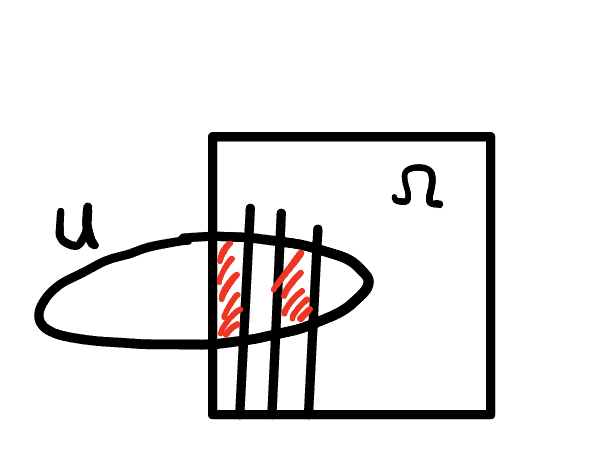
\includegraphics[width=0.2\textwidth]{lem.jpg}
  \caption{例: $\Omega \cap U$有多个连通分支}
\end{figure} 
\begin{proof}
    首先, $V \subsetneq U$ 为开集. 
    注意到, 
    $$ \partial \left( \Omega \cap U \right)=\partial U \cap \overline{\Omega}  \cup \left( \partial \Omega \cap U \right). $$ 
    若 $\partial V \cap U \cap \partial \Omega = \emptyset$, 则 
    $$ \partial V \subset \partial U \cap \overline{\Omega } \subset \partial U ,$$
    于是 $V \subset U$ 为闭集. 由于 $U$ 连通, 所以矛盾.  
\end{proof}
\begin{remark}
    \textcolor{purple}{上述集合运算是在全空间 $\cc^n$ 意义下进行的. 作为开子空间, $\Omega \cap U$ 仍是局部道路连通的, 所以 $V$ 为开集(从而也是 $\cc^n$ 的开集). 另外, 作为拓扑空间 $\Omega \cap U$ 的连通分支, $V$ 相对于 $\Omega \cap U$ 为闭(但不一定是在$\cc^n$中闭). 利用此信息结合假设$\partial V \cap U \cap \partial \Omega = \emptyset$, 可导出 $\partial V \subset \partial U \cap \overline{\Omega }$. }
\end{remark}

\begin{proposition}
    设 $\{K_j\}$ 为 $\Omega $ 中一列紧子集, s.t. $K_j \subset K_{j+1}^{\circ }, \Omega =\cup _j K_j$. 则 存在子列 $\{K_{j_{\nu }}\}$ 以及点列 $\{p_{\nu }\}$ s.t. $p_{\nu } \in K_{j_{\nu +1}}\setminus K_{j_{\nu }}$ 且 $\partial \Omega $ 包含于 $\{p_{\nu }\}$ 的极限点集.       
\end{proposition}
\begin{proof}
    将与 \(\partial\Omega\) 相交的、球心坐标以及半径均为有理数的球全体记为
\(
\{B_{\beta }\},
\)
其为可数集。

由于 \(\Omega\cap B_{\beta }\) 至多有可数个连通分支，故
\[
\mathcal{Q}
:=
\left\{
Q_\alpha:
Q_\alpha \text{ 为某个 } \Omega\cap B_{\beta }
\text{ 的连通分支}
\right\}
\]
为一个可数集。
由引理 \ref{lem4.4}\textcolor{purple}{(确保连通分支不是相对紧? 否则 $j_{\nu }$ 不能任意大)}，存在 \(p_1\in Q_1\)，使得
\[
p_1\in K_{j_1+1}\setminus K_{j_1}.
\]
同理，存在 \(p_2\in Q_2\)，使得
\[
p_2\in K_{j_2+1}\setminus K_{j_2},
\qquad
j_2\gg j_1.
\]
$\dots$\\
$\Rightarrow \exists p_{\nu }\in Q_{\nu }, p_{\nu } \in K_{j_{\nu }+1} \setminus K_{j_{\nu }}, j_{\nu } \geq j_{\nu -1}$. 则 $\{K_{j_{\nu }}\}$ 以及 $\{p_{\nu }\}$ 满足命题条件. 
\end{proof}

\begin{proof}[定理 \ref{thm4.1}, 全纯域 $\Rightarrow $ 全纯凸域]
    只要证 $\forall $ 紧 $K \subset \Omega $: 
    $$ d(\hat{K},\partial \Omega )  \geq d(K,\partial \Omega )~~ (>0) .$$
    ($\Rightarrow $ 等号成立. )   
    设
\[
0<\varepsilon<d(K,\partial\Omega).
\]
于是
\[
K_\varepsilon
:=
\left\{
z:d(z,K)\leq\varepsilon
\right\}
\subset\subset\Omega
\]
为紧集。
设
\[
r=(r_1,\ldots,r_n),
\qquad
r_j>0,
\qquad
\sum_j r_j^2=\varepsilon^2.
\]
则对任意 \(c\in K\)，有
\[
P(c,r)\subset B(c,\varepsilon)\subset K_\varepsilon \subset \subset\Omega.
\]
设 \(f\in\mathcal{O}(\Omega)\)，其在 \(P(c,r)\) 上有 Taylor 展开
\[
f(z)
=
\sum_\alpha
\frac{f^{(\alpha)}(c)}{\alpha!}(z-c)^\alpha.
\qquad (*)
\]
由 Cauchy 不等式，
\[
\left|
\frac{f^{(\alpha)}(c)}{\alpha!}
\right|
\leq
\frac{\sup_{K_\varepsilon}|f|}{r^\alpha}.
\]
于是, 其对任意 \(c\in\widehat{K}\) 也成立. 从而
\[
(*)\text{ 在 }P(c,r)\text{ 中内闭一致收敛},
\quad
\forall\,c\in\widehat{K}.
\]
因为
\[
B(c,\varepsilon)
=
\bigcup_{|r|=\varepsilon}P(c,r).
\]
所以 $f \in \mathcal{O}(B(c,\epsilon )), \forall c \in \hat{K}$. 因为 $\Omega $ 为全纯域, 所以存在 $f \in \mathcal{O}(\Omega )$ 其不能全纯延拓过任一个边界点, 于是 
$$ d(c,\partial \Omega ) \geq \epsilon , \quad \forall c \in \hat{K}. $$  
令
\[
\varepsilon \to  d(K,\partial\Omega).
\]
则
\[
d(c,\partial\Omega)\geq d(K,\partial\Omega),
\]
从而
\[
d(\widehat{K},\partial\Omega)
=
\inf_{c\in\widehat{K}} d(c,\partial\Omega)
\geq
d(K,\partial\Omega).
\]
\end{proof}

\begin{remark}
    实际上, 下面条件 
    $$ (A) \qquad \forall a \in \partial \Omega , \exists f \in \mathcal{O}(\Omega ), s.t. \text{其不能全纯延拓过} a $$
    可以推出全纯凸. 再结合 Cartan-Thullen 定理 $\Rightarrow (A) \iff $ 全纯域. 
\end{remark}

\begin{proposition}
    全纯域 $\Rightarrow $ 拟凸域. 
\end{proposition}
\begin{proof}
取紧穷竭列 \(\{K_j\}\)，使得
\[
K_j=\widehat{K_j},
\qquad
K_j\subset K_{j+1}^{\circ},
\qquad
\Omega=\bigcup_j K_j.
\]
固定 \(j\)。对任意
\(
a\in K_{j+2}\setminus K_{j+1}^{\circ},
\)
存在 \(f_a\in\mathcal{O}(\Omega)\)，使得
\[
\|f_a\|_{L^\infty(K_j)}<1,
\qquad
|f_a(a)|>1.
\]
取 \(a\) 的邻域 \(U_a\)，使得
\[
\inf_{U_a}|f_a|>1.
\]
由 Heine--Borel 定理，存在
\[
f_{j_1},\ldots,f_{j_{m_j}}\in\mathcal{O}(\Omega),
\]
使得
\[
\|f_{j_k}\|_{L^\infty(K_j)}<1,
\qquad \forall\,k,
\]
且
\[
\max_{1\leq k\leq m_j}|f_{j_k}|>1
\quad\text{于 }K_{j+2}\setminus K_{j+1}^{\circ}.
\]

用 \(f_{j_k}^{\,\nu}\)，其中 \(\nu\gg1\)，来代替 \(f_{j_k}\)，使得
\[
\sum_{k=1}^{m_j}|f_{j_k}|^2<2^{-j}
\quad\text{于 }~K_j,
\]
且
\[
\sum_{k=1}^{m_j}|f_{j_k}|^2>j
\quad\text{于 }~K_{j+2}\setminus K_{j+1}^{\circ}.
\]
因此
\[
\rho
:=
\sum_{j=1}^{\infty}
\sum_{k=1}^{m_j}|f_{j_k}|^2
\]
为 \(\Omega\) 上的 \(C^\infty\)  的 $\psh$  穷竭函数。
\end{proof}


\noindent\textbf{Levi 问题}: 拟凸域 $\Rightarrow $ 全纯域? (Oka 解决).

\begin{theorem}[H\"ormander]
    设 $\Omega \subset \subset \cc^n$ 拟凸, $\varphi \in \psh(\Omega )$, $v$ 为 $\Omega $ 上一个 $(0,1)$-形式, s.t. 
    $$ \db v =0 \quad (\text{分布意义})$$
    且 
    $$ \int_{\Omega } |v|^2 e^{-\varphi } <\infty . $$ 
    则 $\db u =v$ 在分布意义下存在解, s.t. 
    $$ \int_{\Omega } \left| u \right| ^2 \frac{e^{-\varphi }}{\left( 1+\left| z \right| ^2 \right)^2} \leq \int_{\Omega } |v|^2 e^{-\varphi } . $$
    若 $v \in C^{\infty }$, 则 $u \in C^{\infty }$. \textcolor{red}{(Carleman 方法)}      
\end{theorem}
\begin{remark}
    \textcolor{red}{涵盖了全纯、多次调和、拟凸。}
   \textcolor{purple}{ (证明可以参考陈伯勇: \textit{Cauchy-Riemann 方程的 $L^2$-理论}.)}
\end{remark}

\begin{proof}[Levi 问题]
    反证法. 假设 $\Omega $ 非全纯域. 则存在 $a \in \partial  \Omega $ 以及邻域 $U \ni a$, s.t. $\forall f \in \mathcal{O}(\Omega )$ 可全纯延拓至 $U$.      

    取 \(p\in \Omega\cap U\) 充分接近边界 \(\partial\Omega\)。
则存在
\[
p^*\in \partial\Omega\cap U,
\]
使得
\[
|p-p^*|=d(p,\partial\Omega).
\]
设 \(H\) 为过 \(p\) 与 \(p^*\) 决定的复直线，其横截 \(\partial\Omega\) 于 \(p^*\)。
不妨设
\[
p^*=0,
\qquad
H=\{z'=0\},
\qquad
z'=(z_1,\ldots,z_{n-1}).
\]
取
\[
f_0(z_n)=\frac{1}{z_n}.
\]
注意到: 若存在
\(
f\in\mathcal{O}(\Omega),
\)
使得
\[
f|_{\Omega\cap H}=f_0,
\]
则与假设矛盾(唯一性定理). 下面来证明 $f$ 的存在性. 

设
\(
\pi:\mathbb{C}^n\to\mathbb{C},
\,
z\mapsto z_n.
\)
取
\(
\chi\in C_0^\infty(\Omega ,\rr),
\)
使得 \(\chi=1\) 于 \(\Omega\cap H \subset \subset\Omega\) 中的一个邻域，
且
\(
\chi=0
\) 于 $\Omega\setminus \pi^{-1}(\Omega\cap H)$ 
中的邻域。
于是
\[
\pi^*f_0\in\mathcal{O}\bigl(\pi^{-1}(\Omega\cap H)\bigr),
\]
故
\[
\chi\cdot \pi^*f_0\in C_0^\infty(\Omega).
\]

令
\[
f:=\chi\cdot \pi^*f_0-u.
\]
为使 \(f\in\mathcal{O}(\Omega)\)，则 \(u\) 应满足
\[
\bar\partial u
=
\bar\partial\bigl(\chi\cdot \pi^*f_0\bigr),
\qquad
u|_{\Omega\cap H}=0.
\]
取
\[
\varphi(z)
=
2(n-1)\log|z'|+\lambda \circ \rho,
\]
其中 \(\rho\) 为 \(\Omega\) 上一个严格 $\spsh$  穷竭函数， \(\lambda\) 凸增。
当 \(\lambda\) 增长足够大时，
\[
\int_\Omega
\left|
\bar\partial\bigl(\chi\cdot \pi^*f_0\bigr)
\right|^2
e^{-\varphi}
<\infty. \quad (\text{\textcolor{red}{练习}})
\]
由 H\"ormander 定理, 方程 $\db u=\db \left( \chi \cdot \pi ^{*} f_{0} \right)$ 存在解, s.t. 
$$ \int |u|^2 \frac{e^{-\varphi }}{\left( 1+\left| z \right| ^2 \right)^2} <\infty . $$ 
因为 $u$ 在 $\Omega \cap H \subset \Omega $ 的某邻域上为全纯, 所以 
$$ u|_{\Omega \cap H}=0 \quad \textcolor{red}{(\text{练习})}. $$  
(因为 $\frac{1}{|z'|^{2n-2}} e ^{-\lambda \circ \rho }$ 有奇性.)
\end{proof}

\begin{remark}
    $$ \int_{\Gamma } \frac{\left| u \right| ^2}{|z'|^{2n-2}}=0 \, \Rightarrow u|_{\{z'=0\}}=0. $$
    (Laurent 级数.)
\end{remark}

\begin{definition}
    设 \(\Omega\) 为 \(\mathbb{C}^n\) 中一个区域，称
\(
\widetilde{\Omega}\subset\mathbb{C}^n
\)
为 \(\Omega\) 的一个（单叶）全纯包，若
\begin{enumerate}[(1)]
  \item 对任意
  \(
  f\in\mathcal{O}(\Omega),
  \)
  \(f\) 可全纯延拓至 \(\widetilde{\Omega}\)；

  \item \(\widetilde{\Omega}\) 为全纯域。
\end{enumerate}
\end{definition}

\begin{example}[Hartogs 圆]
    设 
    $$ H=\{(z_1,z_2) \in \cc^2: |z_1|<1, \frac{1}{2}<\left| z_2 \right| <1\} \cup \{(z_1,z_2): |z_1| <\frac{1}{2},|z_2|<1\} .$$
    则 $\widetilde{H}=\mathbb{D}^2:=\{(z_1,z_2):|z_1|<1,|z_2|<1\}$. 
\end{example}

一般地, 存在 $\Omega \subset \subset \cc^n$, s.t. 全纯包 $\widetilde{\Omega }$ 不存在.  

\begin{example}
设
\(
\Omega\subset\mathbb{C}^2
\)
为
\(
\left\{
|z_1|<1,\ |z_2|<2
\right\}
\)
去掉正方形
\(
I
=
\left\{
0 \leq  x_1<1, y_1=0, |z_2|\leq 1
\right\},
\)
\(
II
=
\left\{
0\leq y_1<1, x_1=0, 1\leq |z_2|<2
\right\}
\)
以及扇形
\(
S
=
\left\{
|z_1|<1, x_1\geq 0, y_1\geq 0, |z_2|<1
\right\}
\)
后所得区域。

\begin{figure}[htbp]
  \centering
  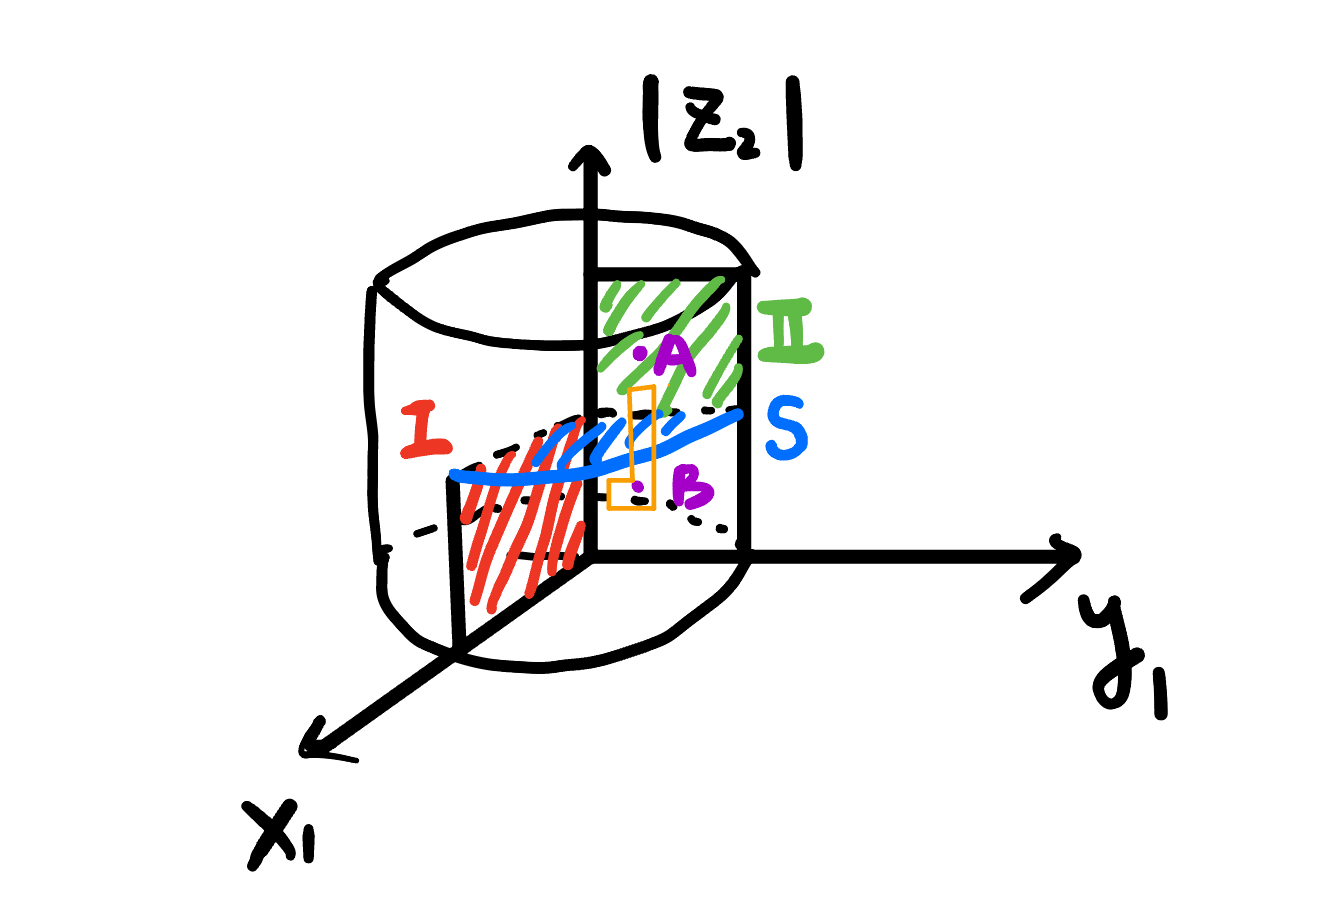
\includegraphics[width=0.4\textwidth]{Riemdom.jpg}
  \caption{$\Omega $ 不存在全纯包}
\end{figure} 
考察 \(\sqrt{z_1}\) 的单值支。
在 \(A,B\) 处取值符号相反。
另一方面，由 Hartogs 延拓，从 \(B\) 到 \(A\) 可延拓过 \(S\)。
因此，延拓后的函数在 \(A\) 处与 \(B\) 处取值相同
$\Rightarrow $  \(\sqrt{z_1}\) 的延拓为多值函数。
故 \(\widetilde{\Omega}\) 不存在！（\textcolor{red}{Riemann 域理论）}
\end{example}





% 附录
\appendix




% 附录
% \appendix
% \chapter{代码}
% \section{代码环境}
% 我们可以在论文中插入算法，但是不建议插入大段的代码。如果确实需要插入代码，建议使用listings宏包。\cite{feynman2011feynman}, \mycite{feynman2011feynman}

% 后置部分包含参考文献、声明页（自动生成）等
\backmatter

% 打印参考文献列表
\printbibliography

% \begin{acknowledgements}
%   致谢
% \end{acknowledgements}

\end{document}
